\documentclass{article}

\usepackage{color}
\usepackage{graphicx}
\usepackage{tabularx}
\usepackage[frenchb]{babel}
\usepackage[utf8]{inputenc}
\usepackage[T1]{fontenc}
\usepackage{lmodern}

\usepackage{geometry,wrapfig,lipsum}
 \geometry{
 top=20mm,
 bottom=20mm,
 }


\title{Document pour l'adaptation des interfaces}
\author{Justal Kevin}
\date{28/09/2015}
\renewcommand{\contentsname}{Table des mati\`eres} 
 
\newcommand\invisiblesection[1]{%
  \refstepcounter{section}%
  \addcontentsline{toc}{section}{\protect\numberline{\thesection}#1}%
  \sectionmark{#1}} 
 
\begin{document}

\begin{center}
\textbf{\Huge{Bootstrap et Polymer}}
\line(1,0){300}\\
DOSSIER D'ANALYSE DES DIFFERENCES\\
\vspace{3cm}
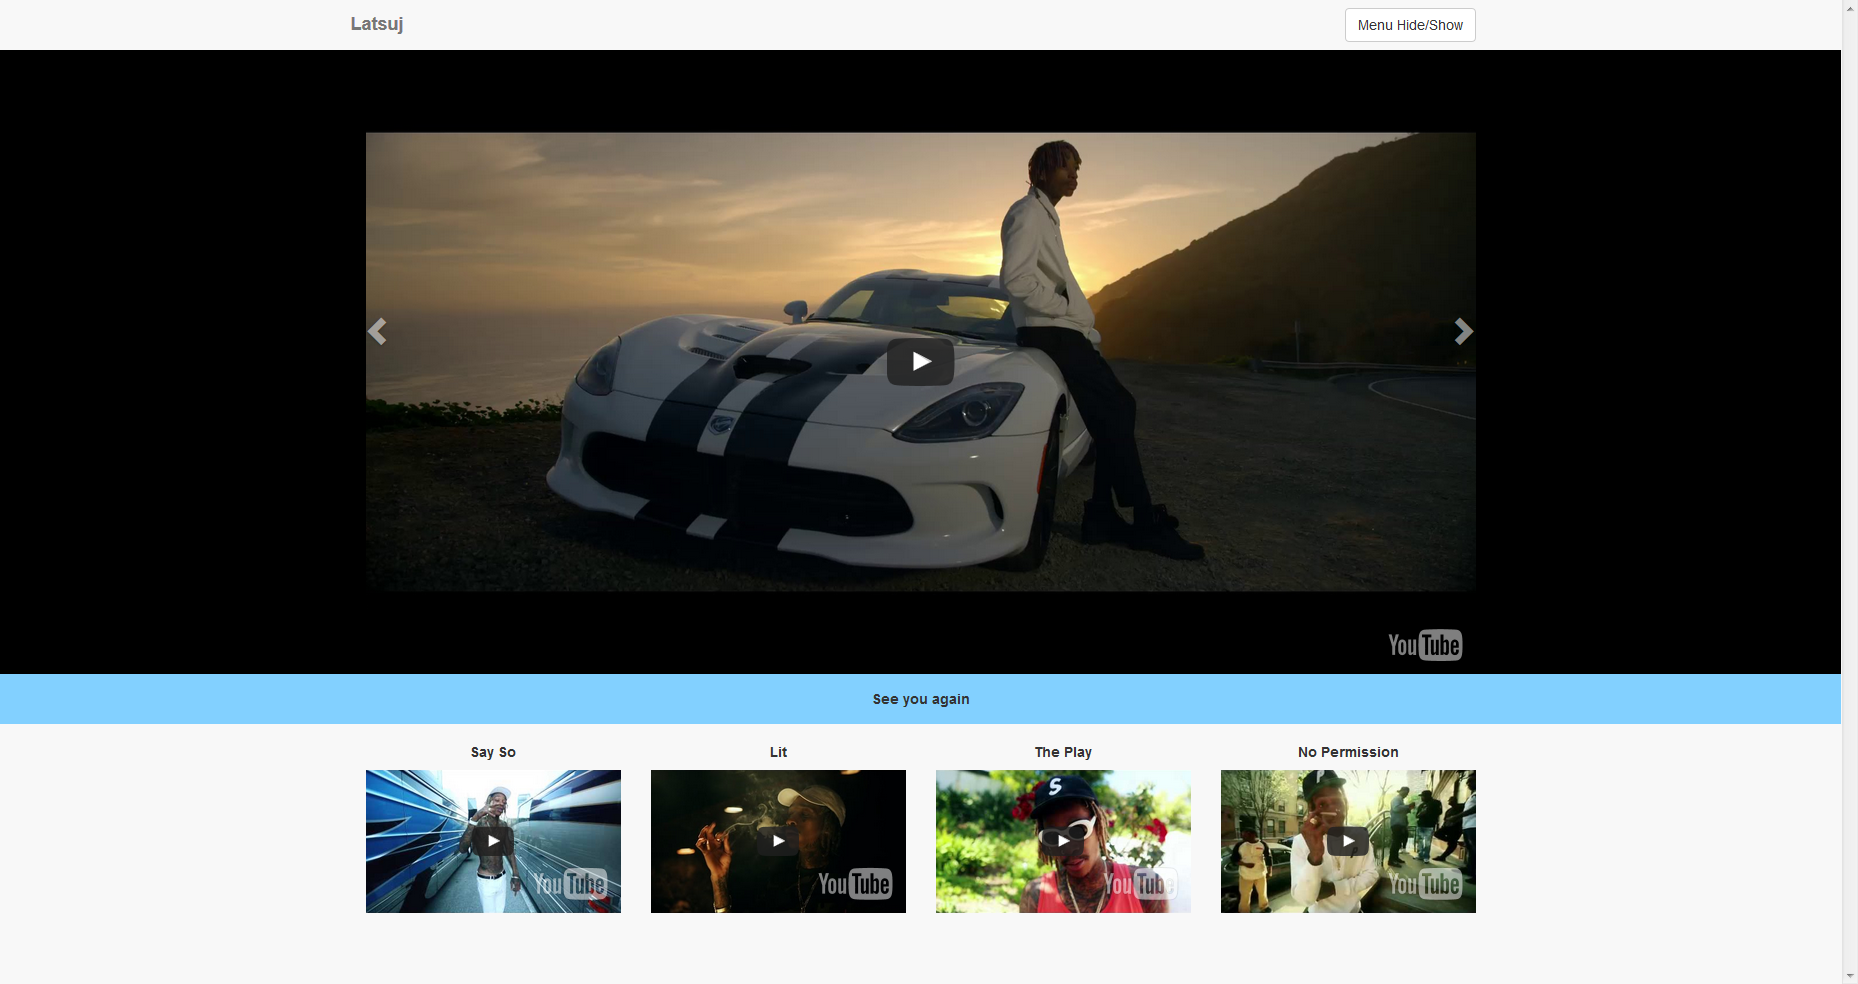
\includegraphics[width=1.0\textwidth]{p1}\\
\vspace{3cm}
\textbf{\Large{JUSTAL KEVIN}}\\
2015\\
\vspace{2cm}
\textbf{Justal Kevin - \color{blue}{\underline{justal@polytech.unice.fr}} \color{black}{- SI5 - IHM}}\\
\vspace{4cm}
\textbf{Enseignant :}\\
\textbf{Anne Marie Dery - \color{blue}{\underline{dery@polytech.unice.fr}}}
\end{center}

\newpage
\section{Pr\'eambule}
\textbf{GitHub}\\
\textit{https://github.com/Latsuj}\\
\vspace{0.5cm}\\
\textbf{Lien de l'exemple}\\
\textit{http://latsuj.com/IHM/Bootstrap}\\
\textit{http://latsuj.com/IHM/Polymer}\\
\vspace{0.5cm}\\
\newpage
\tableofcontents

\newpage

\section{Techniques de conceptions adaptatives utilis\'es}

\begin{wrapfigure}{r}{0.5\textwidth}
  \vspace{-20pt}
  \begin{center}
    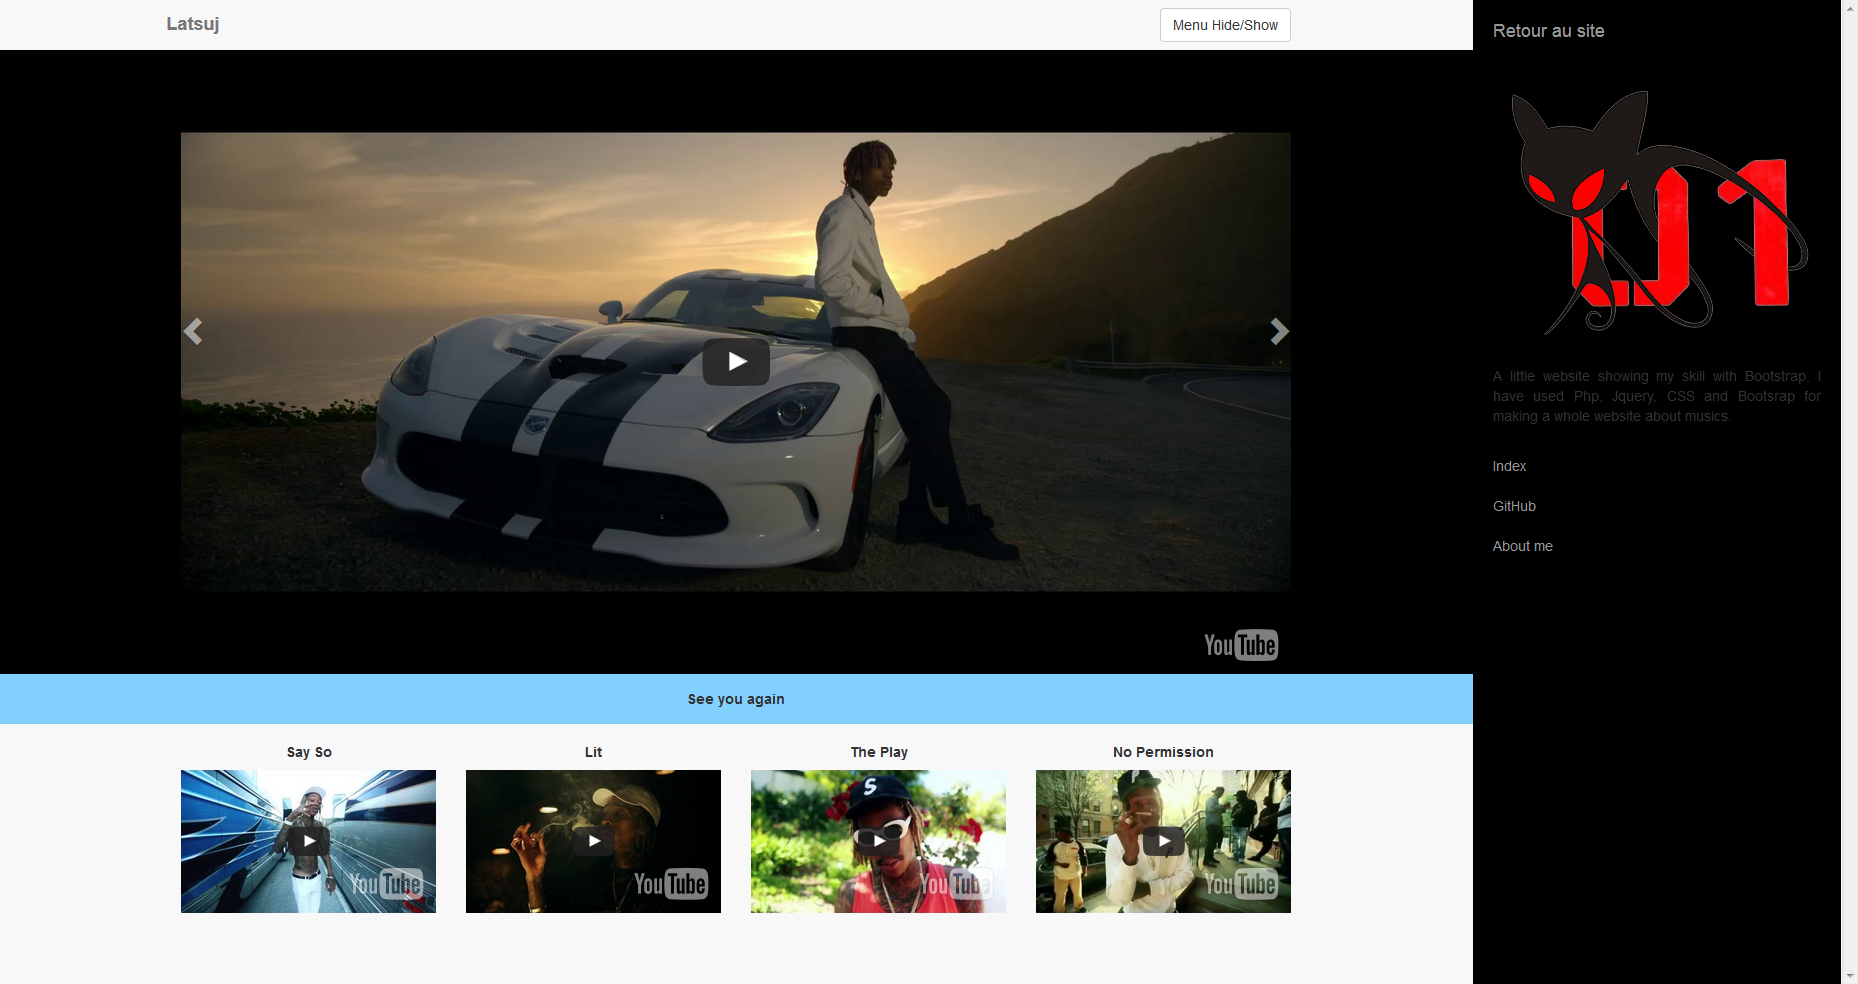
\includegraphics[width=0.48\textwidth]{p2}
  \end{center}
  \vspace{-20pt}
  \caption{Le site pour PC}
  \vspace{-10pt}
\end{wrapfigure}

Pour r\'ealiser mon exemple, je me suis dans un premier temps int\'eress\'e \`a la d\'efinition m\^eme d'un site web adaptatif. Le principe du RWD (\textit{responsive web design}) ou site web adaptatif dans la langue de moli\'ere consiste \`a s'appuyer sur l'usage des \textit{Media queries} que l'on peux aussi appeler \og points de rupture \fg , de grilles de positionnement et d'images flexibles pour rendre un site adaptable \`a son support.\\
Pour d\'evelopper, je suis parti de la version ordinateur \`a une taille relativement imposante, puis j'ai remis en forme les \'el\'ements \`a mesure que la largeur de l'\'ecran diminuait voire je les supprimais totalement. J'ai essay\'e autant que faire se peut d'ajouter un maximum d'\'el\'ements diff\'erents. On retrouve ainsi des vid\'eos, un menu, des tableaux, des images, du texte, des \'el\'ements interactifs comme des boutons... Il y a donc l'ensemble des \'el\'ements que l'on peux retrouver sur n'importe quels sites lambda. \\

\subsection{Structure du site}

\begin{wrapfigure}{l}{0.5\textwidth}
  \vspace{-20pt}
  \begin{center}
    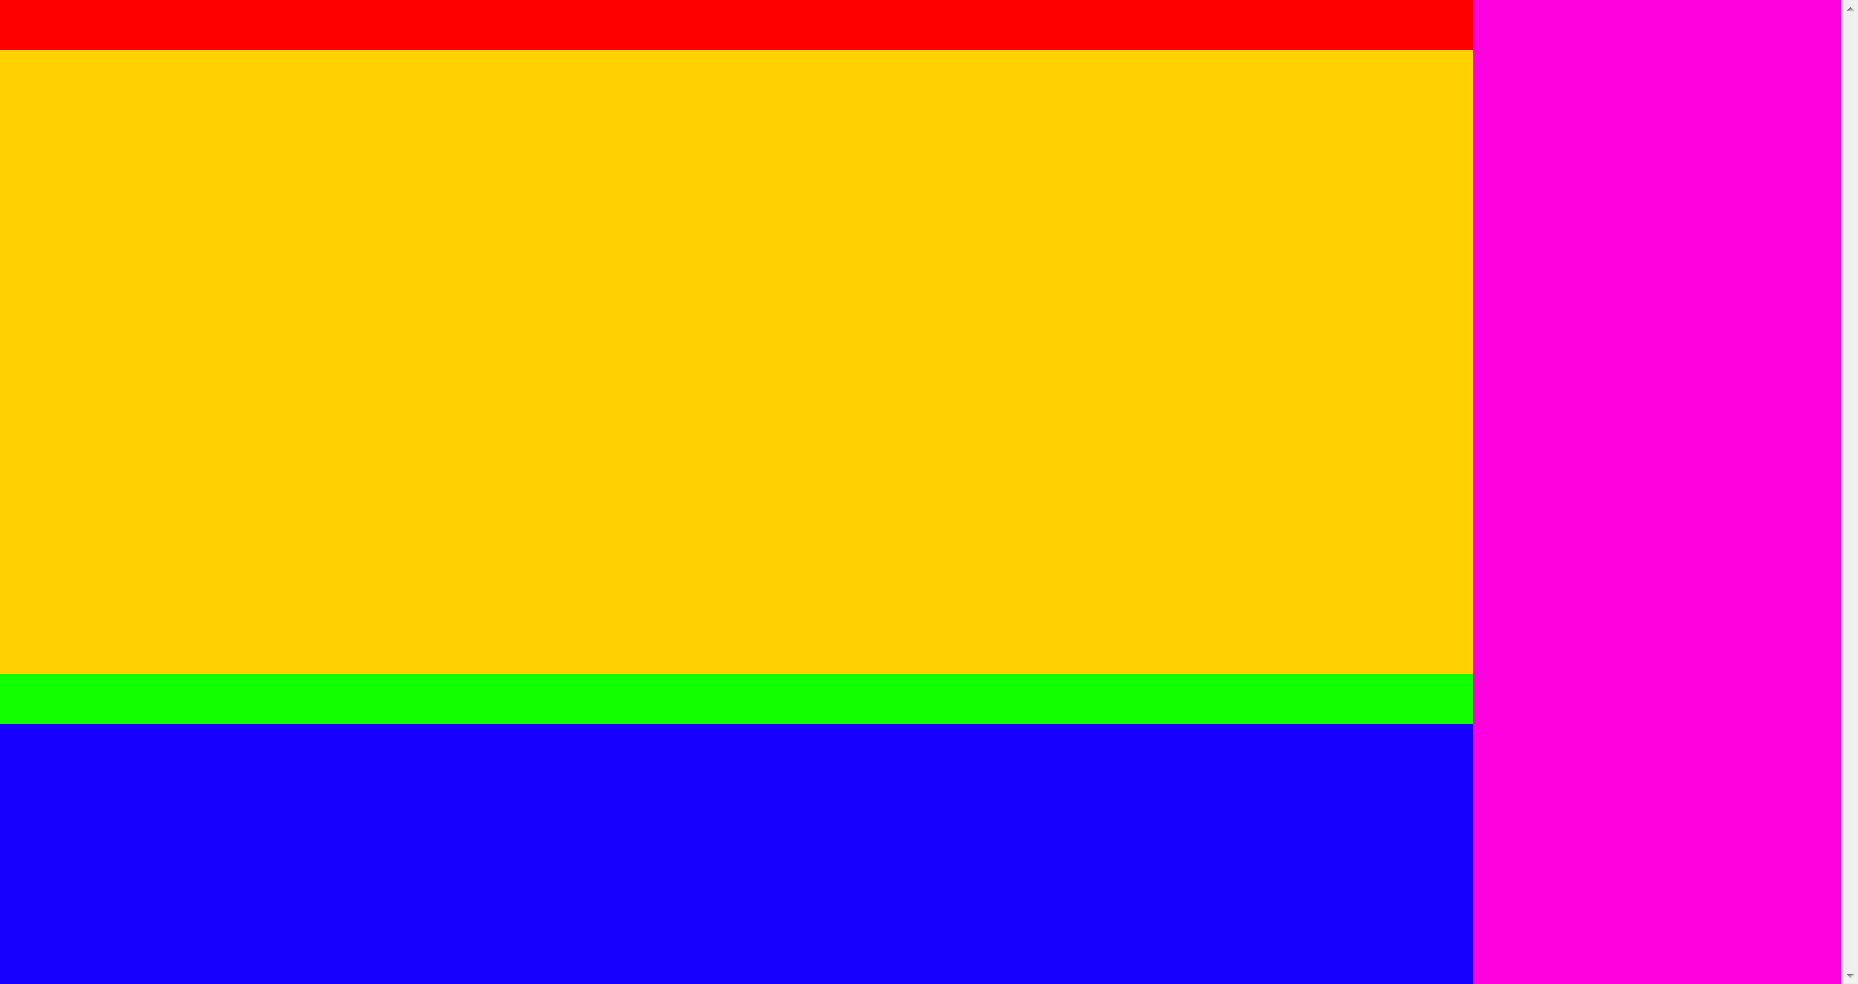
\includegraphics[width=0.48\textwidth]{p3}
  \end{center}
  \vspace{-20pt}
  \caption{Structure du site}
  \vspace{-10pt}
\end{wrapfigure}

Les deux technologies que j'ai choisi partage la m\^eme structure de base. C'est \`a dire un d\'ecoupage en cinq grands blocs. Sur la figure 2, le bloc en rouge repr\'esente la barre principale. En jaune, on retrouve la zone de lecture principale des clips musicaux. En vert, il s'agit d'un bouton permettant d'ouvrir un bloc d'information concernant le clip de la zone jaune. En bleu, il s'agit simplement d'autres clips musicaux en rapport avec le chanteur chantant dans le clip de la zone jaune. En rose, on retrouve un menu que l'on peux ou non afficher gr\^ace \`a un bouton se trouvant dans la zone rouge. Si le menu est rentr\'e, la zone violet n'existe plus et on se retrouve avec seulement quatres blocs qui prendront la totalit\'e de la fen\^etre comme on peux l'observer sur l'image suivante :\\

\begin{center}
  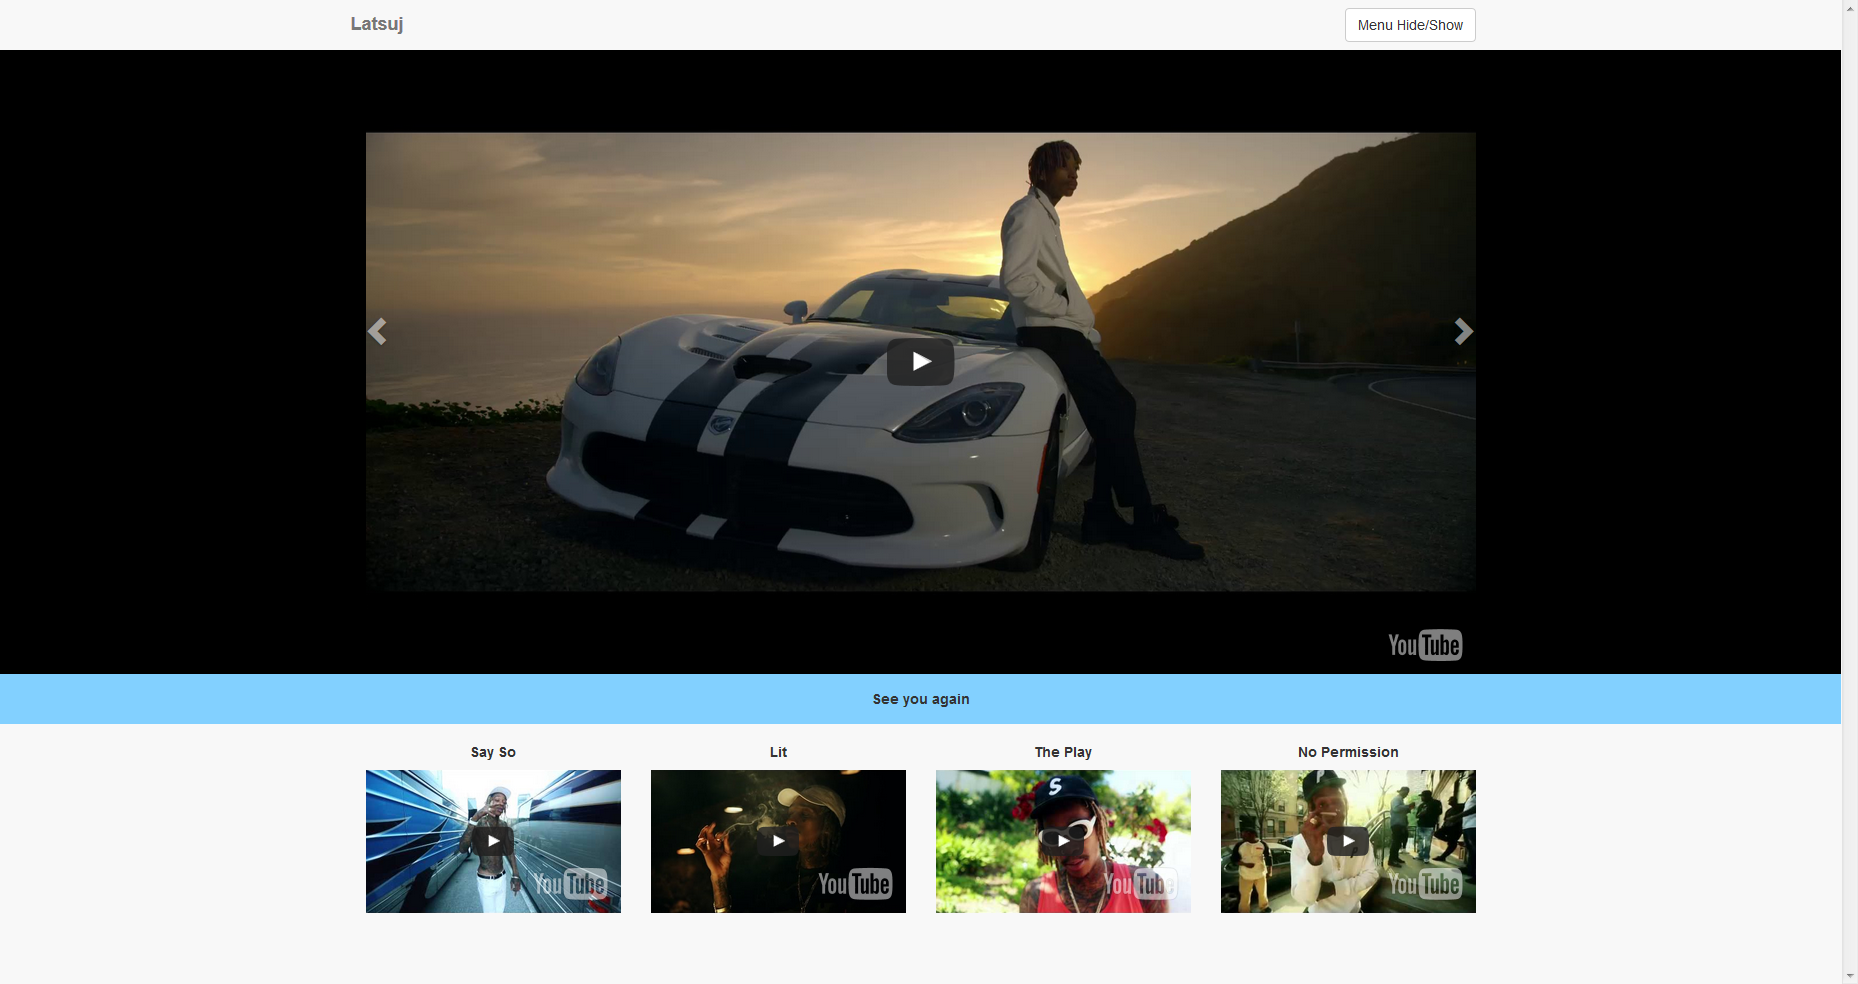
\includegraphics[width=0.8\textwidth]{p1}
\end{center}

\subsection{Images flexibles}

Pour observer pr\'ecis\'ement les diff\'erents principes de RWD sur notre site, nous allons nous int\'erresser \`a certaines zones du site. Pour commencer, nous allons d'abord nous int\'eress\'e au menu (zone violette). Cette derni\'ere illustre \`a la perfection le principe d'image flexible que l'on attend d'un site adaptatif. Qu'est ce qu'une image flexible ? Il s'agit d'une image qui se redimensionnera en fonction de la taille de la fen\^etre. Pour r\'ealiser cela, il faut simplement donner \`a une image quelques attributs CSS. Il faut lui sp\'ecifier de prendre toute la longueur disponible dans le bloc o\`u elle se trouve et de prendre automatiquement une hauteur en fonction de son rapport. En CSS, cela se traduit par : \textit{\og width:100\%;height:auto; \fg{} }. Avec Polymer, j'ai cr\'e\'e un object image qui ajoutait automatiquement des images responsives. Sous Bootstrap, c'est on ne peux plus simple, une classe existe nomm\'e \textit{\og img-responsive \fg} et il suffit de la rajouter sur une balise IMG. Cela permet d'obtenir le r\'esultat suivant lorsque l'on r\'eduit la taille de la fen\^etre :\\

\begin{center}
  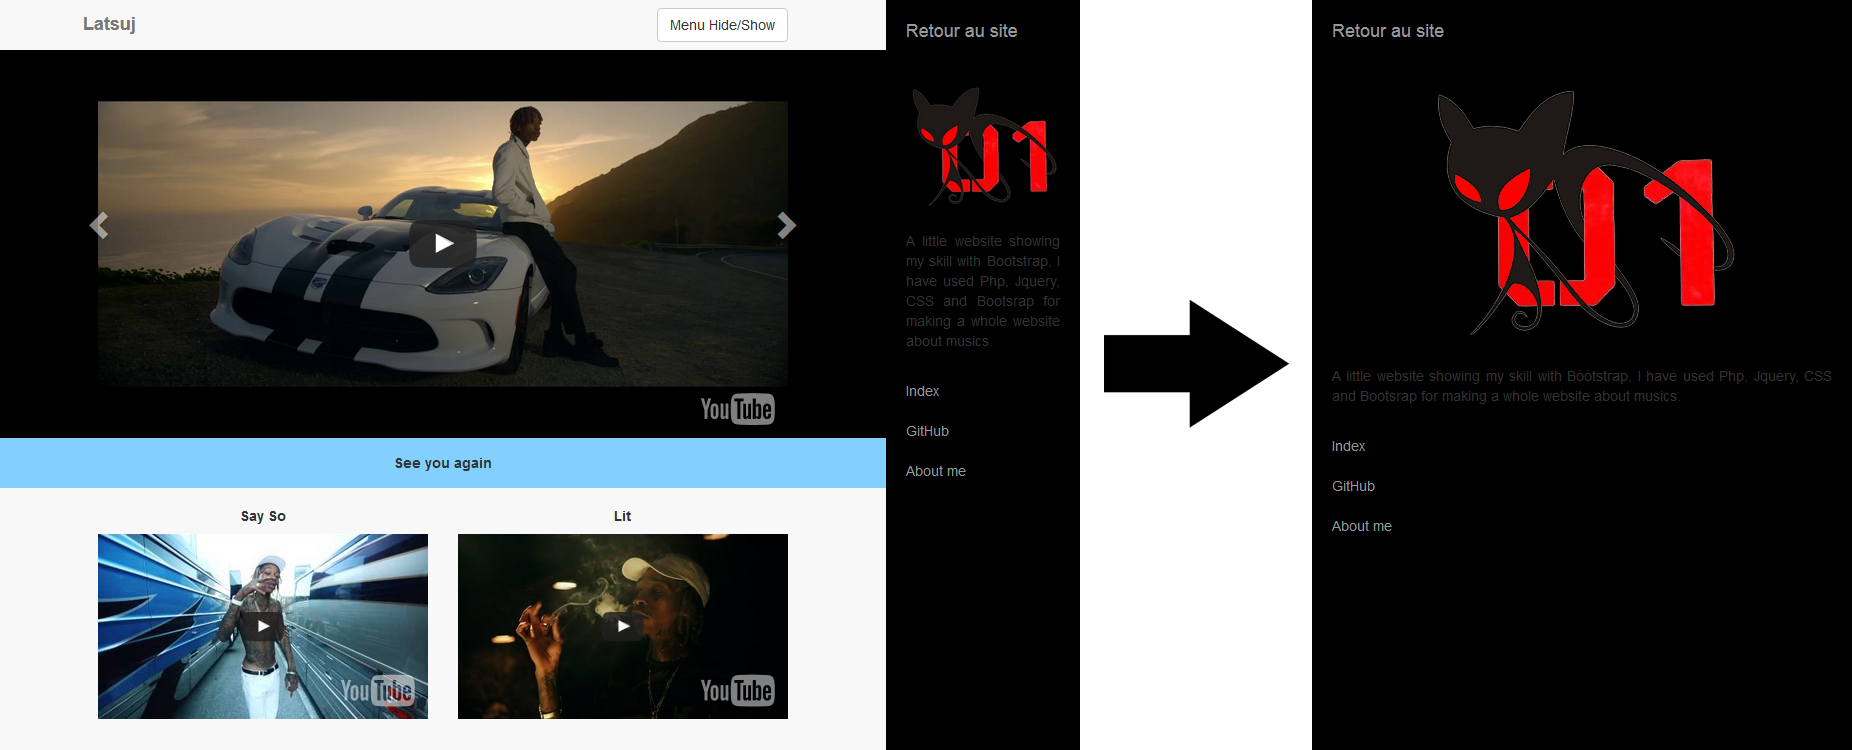
\includegraphics[width=0.8\textwidth]{p4}
\end{center}

Dans mon exemple ci-dessus, on remarque bien que l'image s'adapte \`a la taille de la fen\^etre. On remarque de plus que le site est totalement diff\'erent, il s'agit l\`a de l'application des \textbf{points de rupture} ou \textbf{media queries} dont je parlais pr\'ec\'edemment et que nous allons voir au prochain chap\^itre.

\subsection{Media queries ou Points de rupture}

Les \textbf{media queries} ou points de rupture sont des r\`egles CSS appliqu\'ees en fonction de la largeur de l'\'ecran. Ce sont ces diff\'erentes largeurs qui sont appel\'ees \og points de rupture \fg{}, elles correspondent \`a un besoin de modifier la page \`a partir d'un seuil critique pour la facilitation de la navigation et de la lecture du contenu. Pour que cette d\'efinition soit claire, nous allons montrer leur application sur le site. \\

\begin{wrapfigure}{l}{0.5\textwidth}
  \vspace{-20pt}
  \begin{center}
    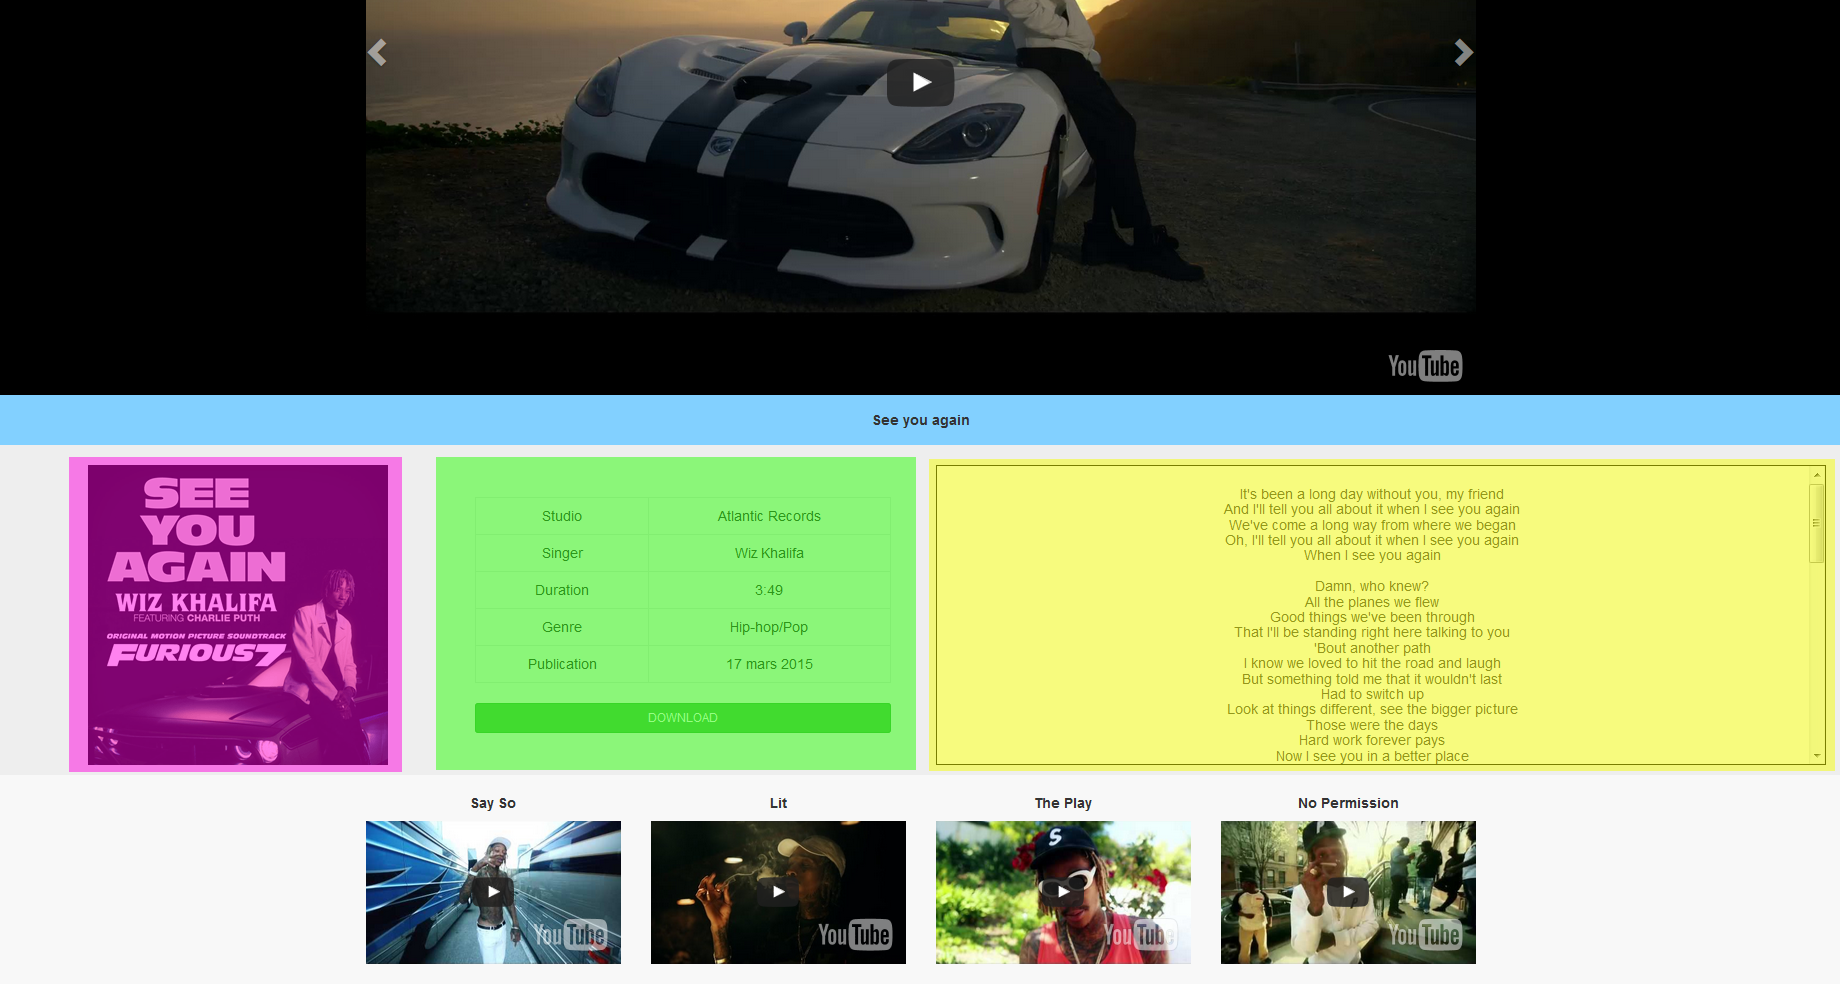
\includegraphics[width=0.48\textwidth]{p5}
  \end{center}
  \vspace{-20pt}
  \caption{Les blocs}
  \vspace{-10pt}
\end{wrapfigure} 

Sur la figure 3, j'ai colori\'e les diff\'erents blocs chacun d'une couleur diff\'erente. Ces blocs sont simplement repr\'esent\'es par des balises DIV avec des r\`egles CSS fonction de la taille de l'\'ecran. Prenons l'exemple du bloc violet, ce bloc fait exactement 25\% du conteneur qui quant \`a lui prend 100\% de la largeur de l'\'ecran. Lorsque l'on r\'eduit la fen\^etre jusqu'\`a un certain point, ce bloc prendra alors 50\% sur ces 100\%. Puis si l'on continue \`a r\'eduire la fen\^etre, ce bloc dispara\^itra.\\  

\begin{center}
  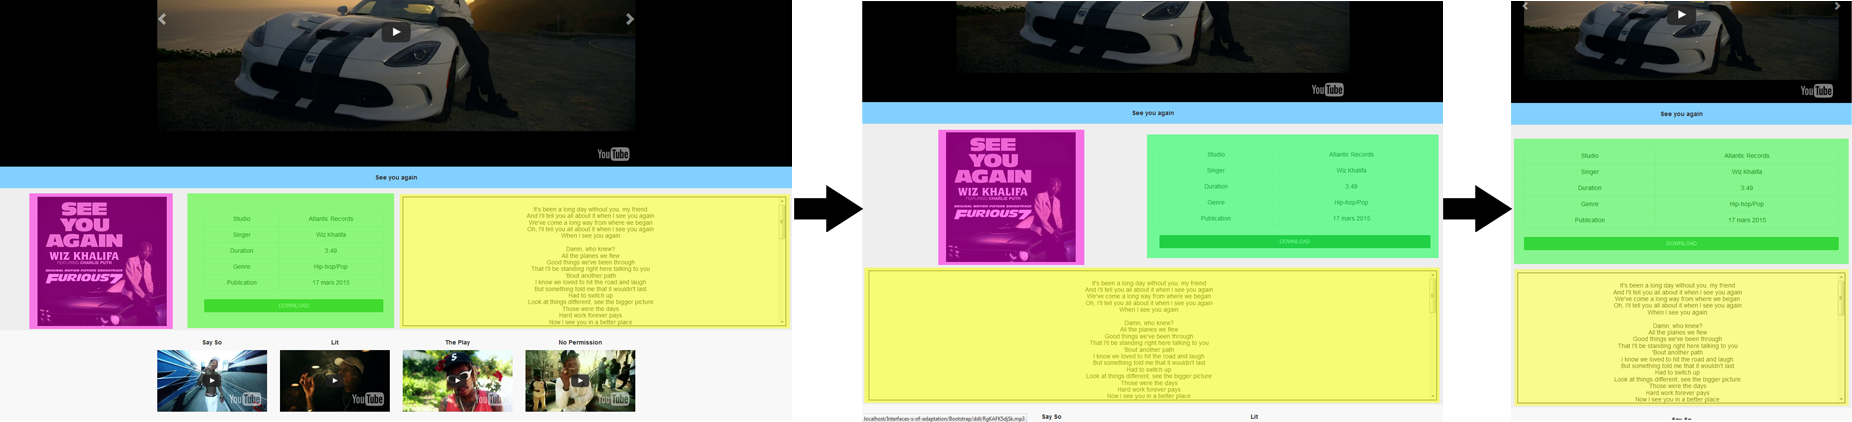
\includegraphics[width=0.8\textwidth]{p8}
\end{center}

Sur Bootstrap, il est assez simple de r\'ealiser ceci. Cette technologie inclue un syst\`eme de grille relativement solide et pratique. Il faut dans un premier temps, d\'efinir notre zone o\`u l'on souhaite r\'ealiser le d\'ecoupage en utilisant la classe \og container \fg{} dans une balise DIV :
\vspace{0.5cm}\\
\fbox{\parbox{\textwidth}{<div class="container">\\
</div>}}
\vspace{0.5cm}
\begin{wrapfigure}{r}{0.5\textwidth}
  \vspace{-20pt}
  \begin{center}
    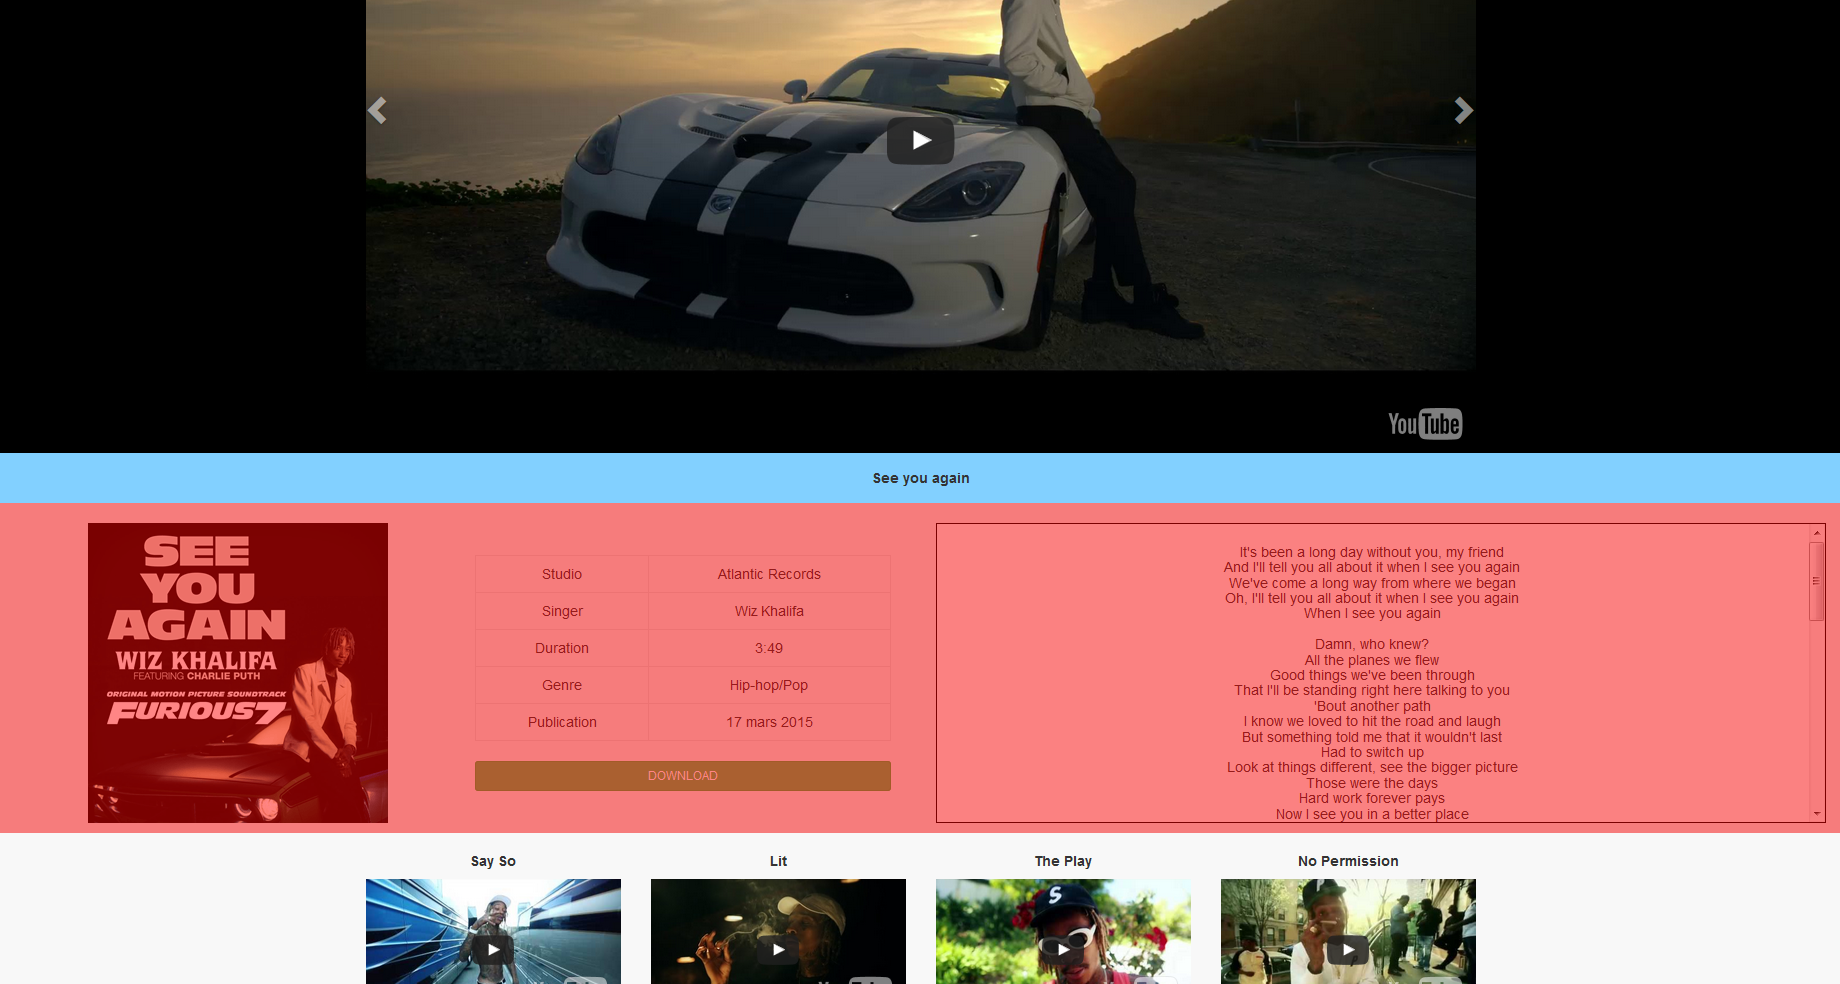
\includegraphics[width=0.48\textwidth]{p9}
  \end{center}
  \vspace{-20pt}
  \caption{Zone du container}
  \vspace{-10pt}
\end{wrapfigure} 
\hspace*{0.6cm}On a ainsi sp\'ecifi\'e o\`u se trouvait notre zone par dessus laquelle nous allons poser une grille. Je n'entrerai dans les d\'etails qu'au chap\^itre suivant, pour l'instant il faut imaginer cela comme une subdivision en 12 parties de la zone rouge sur la figure 4. Comme je l'ai d\'ej\`a expliqu\'e pr\'ec\'edement, l'image dans la zone rouge ne repr\'esente que 25\% de cette zone lorsque l'\'ecran est sup\'erieur \`a 1500px (valeur choisie par mes soins). Ensuite, pour sp\'ecifier \`a Bootstrap que nous allons couper notre container en plusieurs parties, il faut utiliser la classe \og row \fg{} : 
\vspace{0.5cm}\\
\fbox{\parbox{\textwidth}{<div class="container">\\
\hspace*{0.6cm}<div class="row">\\
\hspace*{0.6cm}</div>\\
</div>}}
\vspace{0.5cm}\\
Nous allons maintenant entrer dans le vif du sujet, comme dit plus haut, le container est divis\'e en 12 parties que j'appellerai dans la suite colonne. On peux fixer le nombre de colonnes que peux prendre un \'el\'ement. Reprenons et analysons pr\'ecisement la figure 3, sur cette derni\`ere, la zone jaune prend 6 colonnes et les 6 colonnes restantes sont r\'eparties \'equitablement entre la zone violette et verte. Au niveau du code, on sp\'ecifie cela en utilisant les classes \og col-xs-X \fg,\og col-sm-X \fg,\og col-md-X \fg ou \og col-lg-X \fg. Xs, sm, md et lg repr\'esentent la taille minimum de l'\'ecran pour que les r\`egles que ces classes contiennent prennent effets. Tandis que le X dans ces classes repr\'esente tout simplement le nombre de colonnes que prendra l'\'el\'ement utilisant ces classes. Je reviendrai un peu plus loin sur ce point. Pour l'instant, il est plus important de comprendre la diff\'erence entre les classes xs, sm, md et lg :
\vspace{0.5cm}\\
\fbox{\parbox{\textwidth}{<div class="container">\\
\hspace*{0.6cm}<div class="row">\\
\textbf{\hspace*{1.2cm}\color{red}{<div class="col-md-12 col-lg-6">}}\\
\hspace*{1.8cm}<div class="row">\\
\textbf{\hspace*{2.4cm}\color{blue}{<div class="hidden-xs hidden-sm col-md-6 col-lg-6>}}\\
\hspace*{3.0cm}...\\
\hspace*{2.4cm}</div>\\
\hspace*{2.4cm}...\\
\hspace*{1.8cm}</div>\\
\hspace*{1.2cm}</div>\\
\hspace*{1.2cm}...\\
\hspace*{0.6cm}</div>\\
</div>}}
\vspace{0.5cm}\\
Ce bout de code est suffisant pour comprendre et expliquer clairement les mouvements de l'image violette dans la figure 3. Le texte en rouge pr\'ecise qu'\`a grande taille lg (sup\'erieur \`a 1500px), la zone violette et verte ont 50\% du container, soit 6 colonnes : \og col-lg-6 \fg{} . Le texte en bleu est la balise DIV directe qui contient l'image violette. Ces classes sp\'ecifient qu'\`a grande taille, ce bloc ne peux exc\'eder 6 colonnes, soit 50\%. Or, 50\% de 50\% fait bien 25\% comme je l'avais dit plus haut. Cependant cela n'est valide que lorsque la fen\^etre est sup\'erieur \`a 1500px. En dessous, les autres classes prennent le relais.\\ 

\begin{wrapfigure}{r}{0.5\textwidth}
  \vspace{-20pt}
  \begin{center}
    \begin{tabular*}{0.48\textwidth}{@{\extracolsep{\fill}} | c | l | }
  \hline
  xs & 600px\\
  \hline
  sm & 900px\\
  \hline
  md & 1200px\\
  \hline
  lg & 1500px\\
  \hline
\end{tabular*}
  \end{center}
  \vspace{-20pt}
  \caption{Points de rupture}
  \vspace{-10pt}
\end{wrapfigure} 

Pour comprendre pr\'ecisement quelles sont les classes qui sont actives \`a une grandeur de fen\^etre donn\'e, il faut simplement retenir les dimensions que repr\'esentent les sigles xs, sm, md, lg. Les dimensions qui sont affich\'ees ne sont pas celles par d\'efauts de Bootstrap mais celles que j'ai utilis\'e pour mon site. J'ai chang\'e les points de rupture pour que mon menu puisse s'ins\'erer joliment sur mon site. Sans cela, il se pouvait que le bouton de la barre de menu chevauche le menu, ce qui donnait un r\'esultat plut\^ot moche. La seule mani\`ere de r\'egler le probl\`eme a \'et\'e de construire une version personnalis\'e de Boostrap. Il est possible d'effectuer cette op\'eration sur le site officiel de Bootstrap.\\

\begin{wrapfigure}{l}{0.5\textwidth}
  \vspace{-20pt}
  \begin{center}
    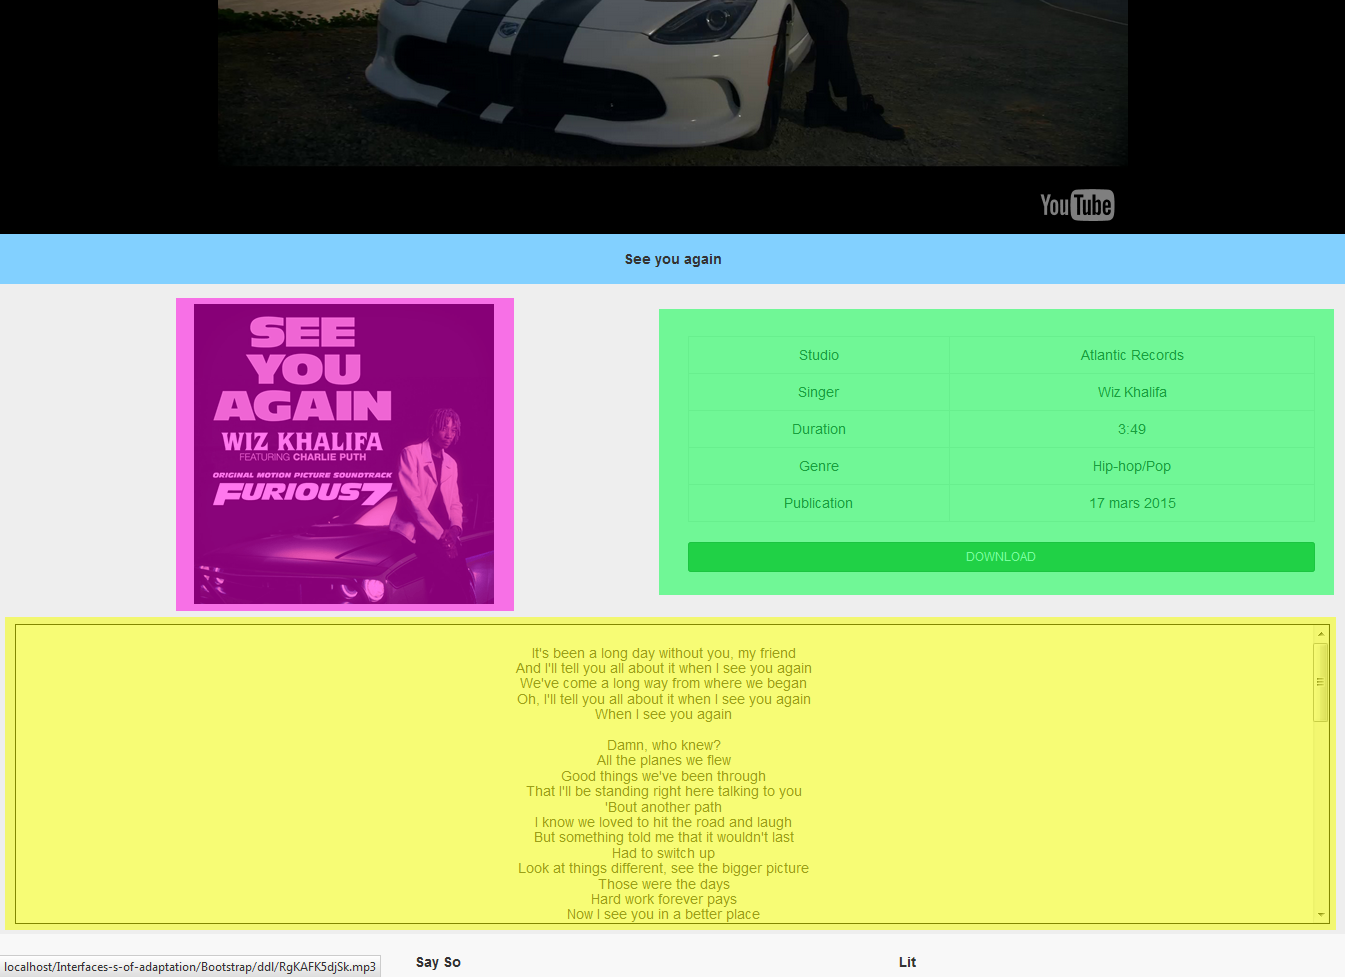
\includegraphics[width=0.48\textwidth]{p6}
  \end{center}
  \vspace{-20pt}
  \caption{50\% de la fen\^etre}
  \vspace{-10pt}
\end{wrapfigure} 

Dans notre cas, si la fen\^etre est inf\'erieur \`a 1500px alors les classes lg ne sont plus utilis\'ees. Prenons une fen\^etre de 1300px, si l'on regarde le tableau de la figure 5, on remarque que pour toutes les dimensions situ\'ees entre 1200 px et 1500 px, md est la classe qui est actif. On reprend notre bout de code pr\'ec\'edent et on remarque que le texte en rouge mentionne \og col-md-12 \fg{}. Cela signifie que cette div qui repr\'esente la zone violette et verte de la figure 3 prendra 100\% du container. On regarde notre texte en bleu et on lit \og col-md-6 \fg{}. L'image violette prendra donc 50\% de 100\%, elle prendra donc la moiti\'e de la longueur de la fen\^etre.\\

\newpage
\begin{wrapfigure}{l}{0.5\textwidth}
  \vspace{-20pt}
  \begin{center}
    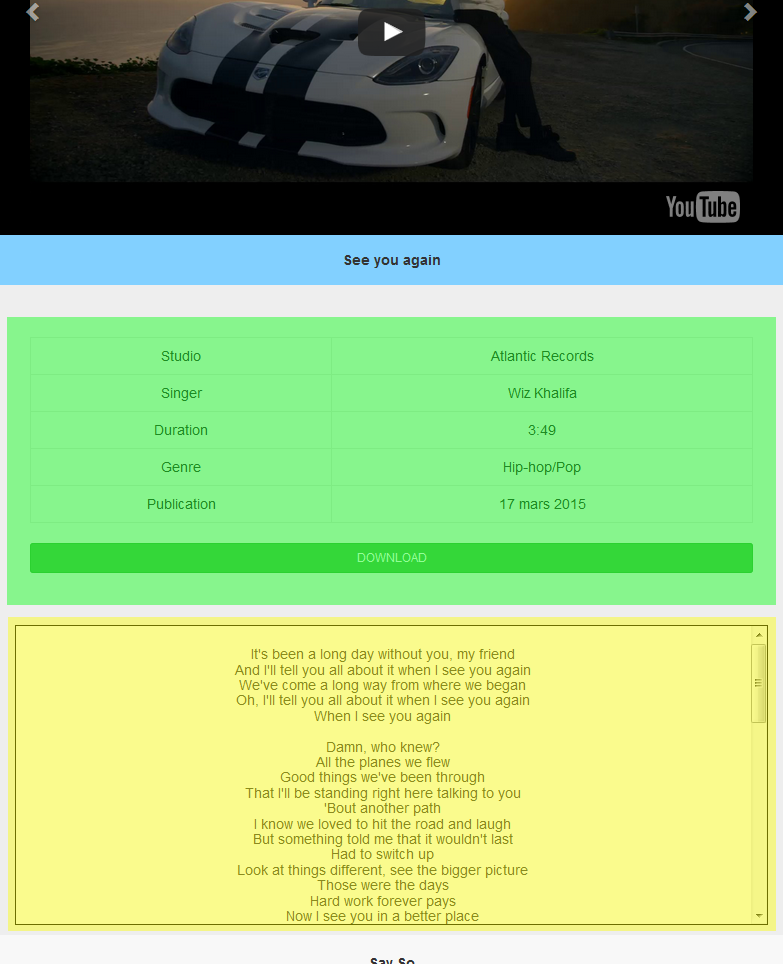
\includegraphics[width=0.48\textwidth]{p7}
  \end{center}
  \vspace{-20pt}
  \caption{L'image a disparu}
  \vspace{-10pt}
\end{wrapfigure} 

Si nous continuons de r\'eduire la fen\^etre et atteignons une taille inf\'erieur \`a 1200px, nous arrivons dans les classes sm. Si on regarde le texte en bleu dans le bout de code pr\'ec\'edent, on voit qu'il est \'ecrit \og hidden-sm \fg{}. Cette classe signifie que le nombre de colonnes pris par cet \'el\'ement sera r\'eduit \`a z\'ero. Cela se traduit par une disparition compl\`ete de l'\'el\'ement comme on peux le voir sur la figure 7. Notons au passage que je n'ai pas pr\'ecis\'e dans le texte en rouge le nombre de colonne pour les dimensions sm et xs. Je n'ai pas eu \`a le faire car Bootstrap utilise les r\`egles CSS pour r\'ealiser ces modifications. Plus pr\'ecisement, Bootstrap utilise l'h\'eritage et le cascading de CSS pour pouvoir r\'e\'ecrire des r\`egles sur des r\`egles. Si on ne d\'efinit pas de xs, alors les r\`egles CSS seront celles de sm. Si elles aussi ne sont pas d\'efinis, alors ce seront celles de md qui seront prise en compte...Cela ne constitue pas une faute mais j'aurai pu omettre le \og col-md-6 \fg{} dans mon texte bleu et cela donnerai toujours le m\^eme r\'esultat.\\

Nous avons vu comment mettre cela en place sur Bootstrap, on peux \'evidemment faire la m\^eme chose avec Polymer. Le r\'esultat obtenu est le m\^eme mais la mani\`ere d'y arriver est diff\'erente. Cependant, notons que cela est totalement contraire \`a l'id\'ee de Polymer. J'ai discut\'e de cela avec Monsieur Bidelman lui-m\^eme qui est un des fondateurs de Polymer et qui travaille actuellement chez Google. Le but est de cr\'eer des \'el\'ements r\'eutilisables. Or \`a partir du moment o\`u l'on utilise des m\'edias queries, l'\'el\'ement devient ancr\'e au site qui les utilisent. Prenons l'exemple pr\'ec\'edent, pour que l'image disparaisse \`a un certain point de rupture, j'ai cr\'e\'e un \'el\'ement qui change son attribut \og display \fg{} lorsque l'on atteint ce fameux point.
\vspace{0.5cm}\\
\fbox{\parbox{\textwidth}{
<dom-module id="my-col-hidden-900">\\
\hspace*{0.6cm}<template>\\
\hspace*{1.2cm}<style>\\				
\hspace*{1.8cm}\color{blue}{@media (max-width:900px) \{\\
\hspace*{2.4cm}:host \{\\
\hspace*{3.0cm}display: none;\\
\hspace*{2.4cm}\}\\
\hspace*{1.8cm}\}\\
\hspace*{1.2cm}}\color{black}{</style>\\
\hspace*{1.2cm}<content></content>\\
\hspace*{0.6cm}</template>\\
\hspace*{0.6cm}<script>\\
\hspace*{1.2cm}Polymer({\\
\hspace*{1.8cm}is: "my-col-hidden-900"\\
\hspace*{1.2cm}});\\
\hspace*{0.6cm}</script>\\
</dom-module>}}}
\vspace{0.5cm}\\
On a donc cr\'e\'e une nouvelle node HTML dans le DOM nomm\'e my-col-hidden-900. Le code en bleu est la partie la plus importante. Elle sp\'ecifie que le code se situant entre les balises \og my-col-hidden-900 \fg{} aura l'attribut \og display:none \fg{} si la taille de la fen\^etre est inf\'erieur \`a 900px. Autrement dit, tout le contenue \`a l'int\'erieur ne sera pas affich\'e.\\
Dans le m\^eme style, j'ai cr\'e\'e un \'el\'ement du DOM dont la longueur s'adapte en fonction la largeur de la fen\^etre. La largeur ainsi que le position naturel des balises DIV avec l'attribut \og float:left \fg{} permet de r\'ealiser un semblant de grille sous Polymer :
\vspace{0.5cm}\\
\fbox{\parbox{\textwidth}{
<dom-module id="my-col-25-100">\\
\hspace*{0.6cm}<template>\\
\hspace*{1.2cm}<style>\\
\hspace*{1.8cm}\color{blue}{:host \{	\\	
\hspace*{2.4cm}position: relative;\\
\hspace*{2.4cm}min-height: 1px;\\
\hspace*{2.4cm}padding-left: 15px;\\
\hspace*{2.4cm}padding-right: 15px;\\
\hspace*{2.4cm}float:left;\\
\hspace*{2.4cm}width:25\%;\\
\hspace*{2.4cm}box-sizing: border-box;\\
\hspace*{1.8cm}\} }\\
\hspace*{1.8cm}\color{red}{@media (max-width:1500px) \{\\
\hspace*{2.4cm}:host \{\\
\hspace*{3.0cm}width:50\%;\\
\hspace*{2.4cm}\}\\
\hspace*{1.8cm}\}}	\\	
}}\\
\fbox{\parbox{\textwidth}{
\hspace*{1.8cm}\color{green}{@media (max-width:900px) \{\\
\hspace*{2.4cm}:host \{\\
\hspace*{3.0cm}width:100\%;\\
\hspace*{2.4cm}\}\\
\hspace*{1.8cm}\}}		\\
\hspace*{1.8cm}\color{black}{</style>\\
\hspace*{1.8cm}<content></content>\\
\hspace*{0.6cm}</template>\\
\hspace*{0.6cm}<script>\\
\hspace*{1.2cm}Polymer(\{\\
\hspace*{1.8cm}is: "my-col-25-100"\\
\hspace*{1.2cm}\});\\
\hspace*{0.6cm}</script> \\ 
</dom-module>}}}
\vspace{0.5cm}\\

\begin{wrapfigure}{r}{0.5\textwidth}
  \vspace{-20pt}
  \begin{center}
    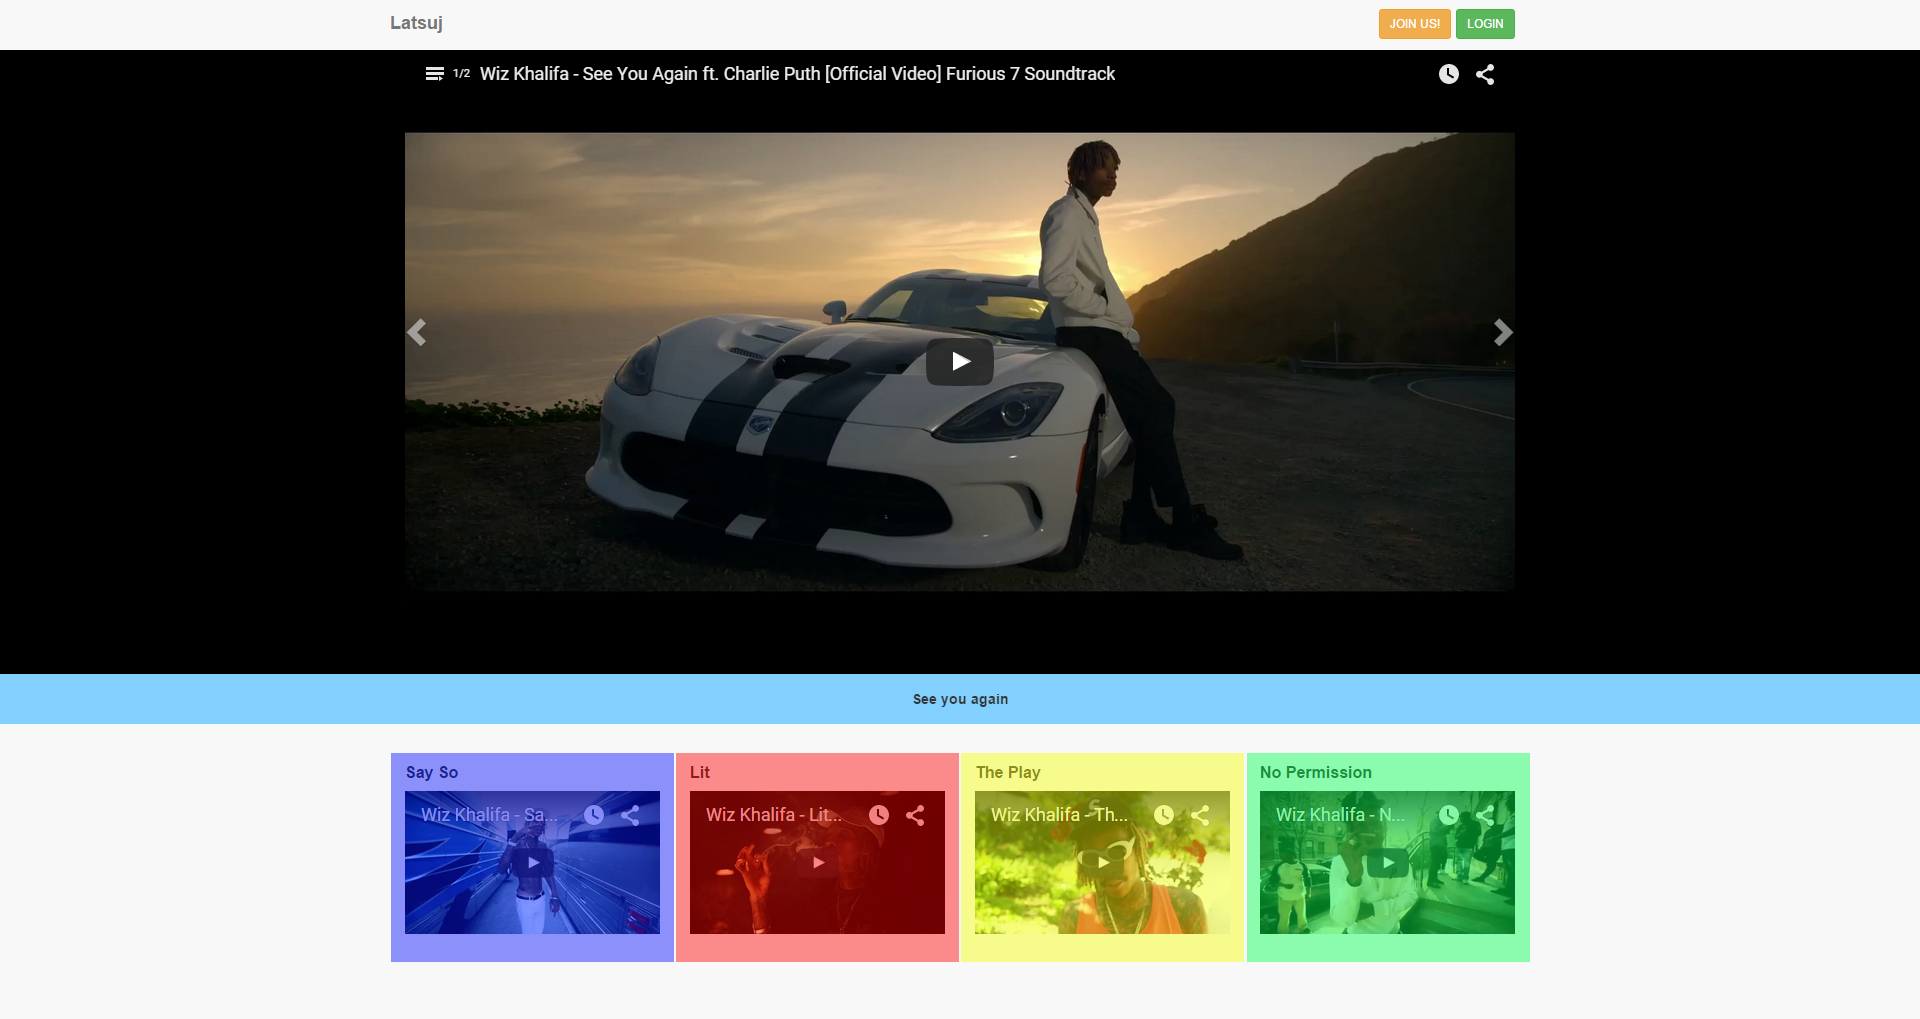
\includegraphics[width=0.48\textwidth]{pc4}
  \end{center}
  \vspace{-20pt}
  \caption{Les 4 blocs}
  \vspace{-10pt}
\end{wrapfigure} 

Ce module permet d'ajouter une nouvelle node HTML nomm\'e \og my-col-25-100 \fg{}. Cette derni\`ere permet de faire la division et le repositionnement des clips musicaux en bas de page. J'ai colori\'e chacun des \'el\'ements utilisant ce module sur la figure 8. Sur cette figure, la dimension de la fen\^etre est sup\'erieur \`a 1500px. Dans le code pr\'ec\'edent, les r\`egles en bleu sont celles actives. On remarque que la taille (\og width \fg{} ) est sp\'ecifi\'e \`a 25\% du container. Chacun des clips prend donc 25\%, ce qui apparait bien sur la figure \`a droite. Ensuite, si l'on r\'eduit la fen\^etre, nous arriverons au point d'ancrage \`a 1500px. Les r\`egles appliqu\'ees seront donc celles \'ecrites en bleu puis en rouge. Les r\`egles rouges donneront de nouvelles valeurs aux r\`egles en bleu, elles seront r\'e\'ecrites. Dans notre cas, la largeur maximale que pourra prendre un de nos clips musicaux sera de 50\% du container. Ainsi, lorsque 100\% du container est pris par 2 vid\'eos, les suivantes se placeront en dessous. Maintenant, imaginons que nous continuons \`a r\'eduire la fen\^etre jusqu'au point de rupture \`a 900px, chaque vid\'eos prendra la totalit\'e de la largeur de la fen\^etre. L'image ci-dessous montre le r\'esultat obtenu via ces points de rupture avec les modules pr\'ec\'edents :

\begin{center}
\vspace{0.5cm}
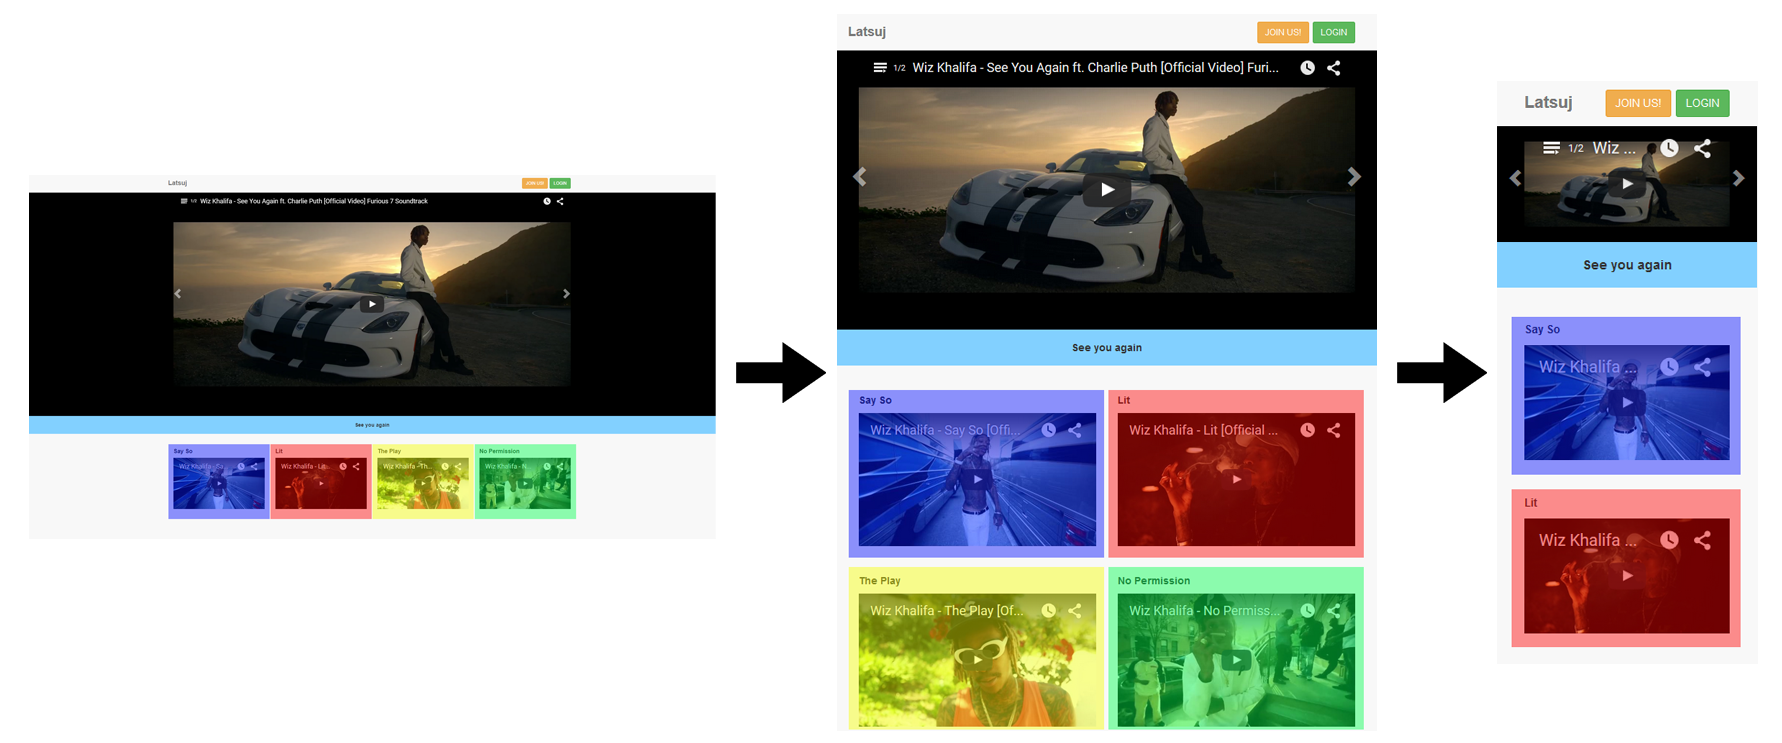
\includegraphics[width=0.8\textwidth]{pc7}
\vspace{0.5cm}\\
\end{center}

\`A travers ces diff\'erents exemples, nous avons pu voir comment faire des points de rupture sous les deux technologies diff\'erentes. Sur Bootstrap, il est bien plus simple d'utiliser ces points de rupture. L'utilisation des classes xs, sm, md et lg rendent le principe facile \`a comprendre. Cependant, nous sommes limit\'e par Bootstrap \`a suivre ces quatres points de rupture. Si le site contient de nombreux autres points de rupture, Bootstrap perd de sa superbe car cela reviendrait \`a faire du CSS classique. Sur Polymer, il faut bien comprendre les m\'edia queries (points de rupture) pour pouvoir les utiliser. Comme Polymer fractionne notre code, on se retrouve avec du CSS et donc des points de rupture qui se retrouvent \'eparpill\'e dans le code. En cas de changement de points de rupture, la maintenance peut vite devenir difficile. 

\subsection{Grille de positionnement}

\begin{wrapfigure}{r}{0.5\textwidth}
  \vspace{-25pt}
  \begin{center}
    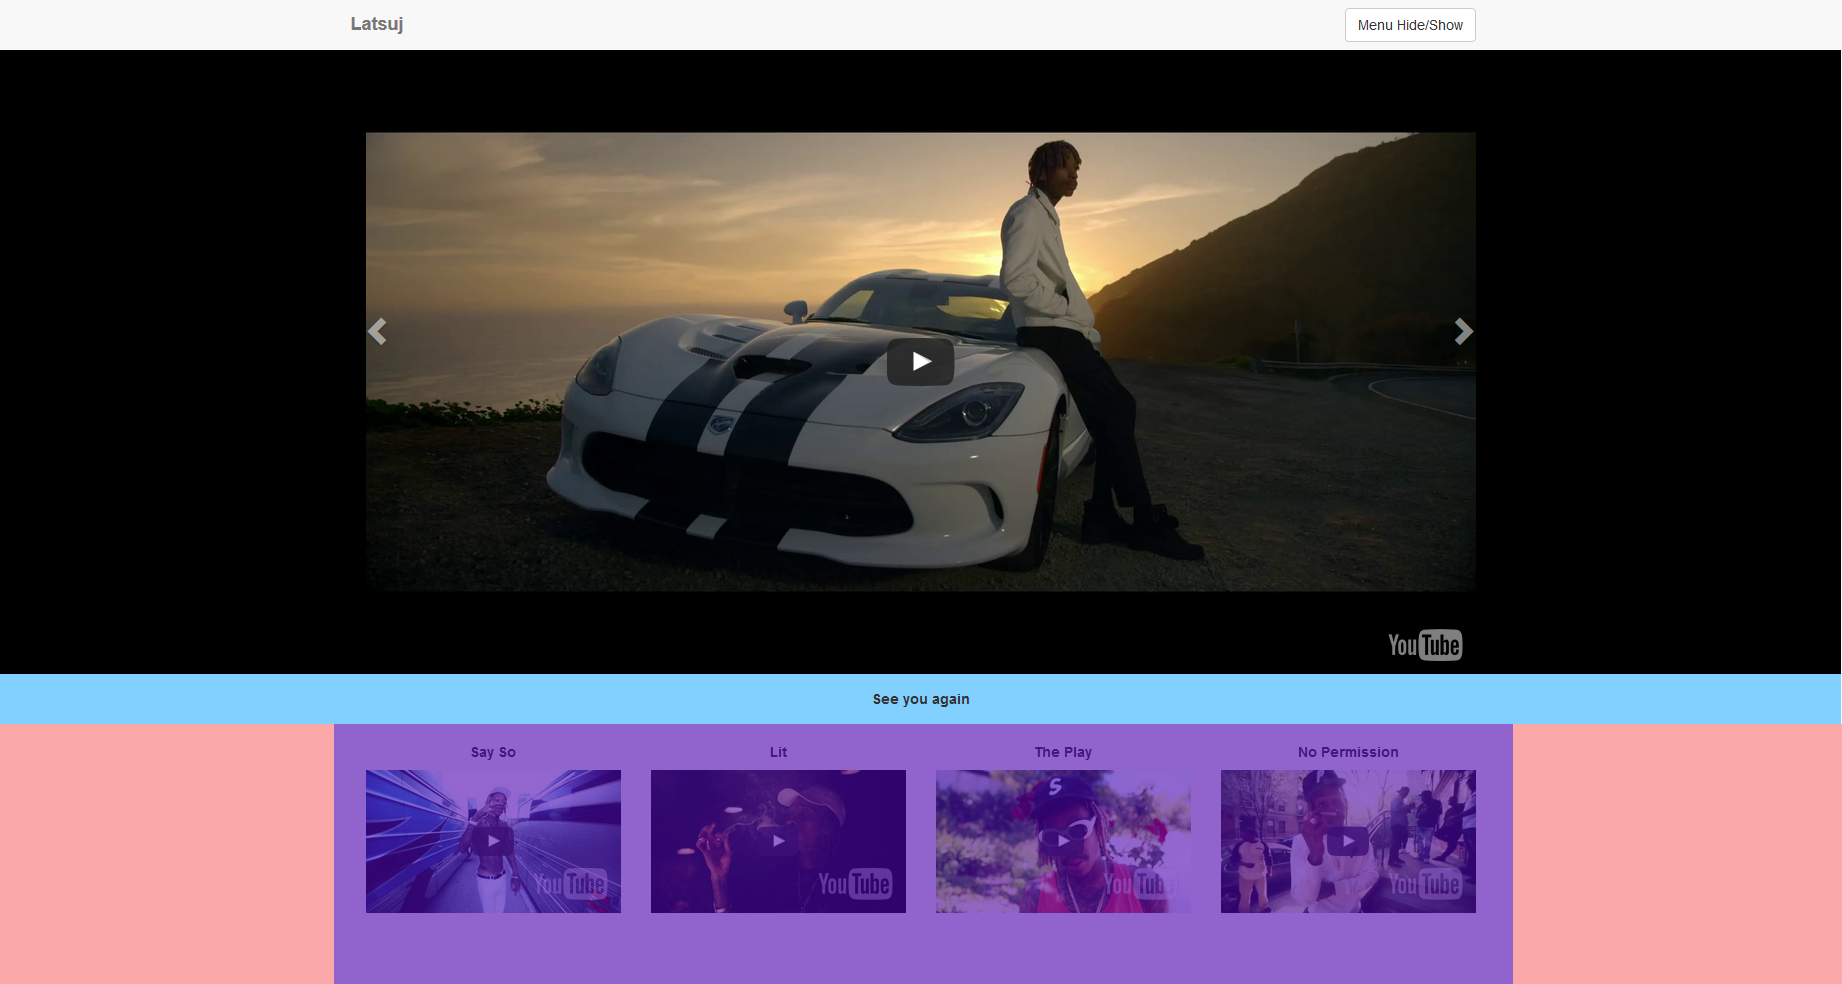
\includegraphics[width=0.48\textwidth]{p10}
  \end{center}
  \vspace{-20pt}
  \caption{Le container du bas de page}
  \vspace{-10pt}
\end{wrapfigure} 

Les grilles de positionnement consistent en un dimensionnement relatif des diff\'erents blocs de la page. J'ai d\'ej\`a partiellement \'evoqu\'e ce point. Je vais essayer de me concentrer ici sur ce point en particulier. Comme dit dans le chap\^itre pr\'ec\'edent, les grilles se placent dans des containers. Qu'est qu'un container ? Sur la figure 9, j'ai repr\'esent\'e en violet, le container du bas de la page. On peux aussi l'obtenir en analysant le code avec Firebug (F12). Cet espace violet est la place maximale que peux prendre le contenue ici.\\

\begin{wrapfigure}{r}{0.5\textwidth}
  \vspace{-25pt}
  \begin{center}
    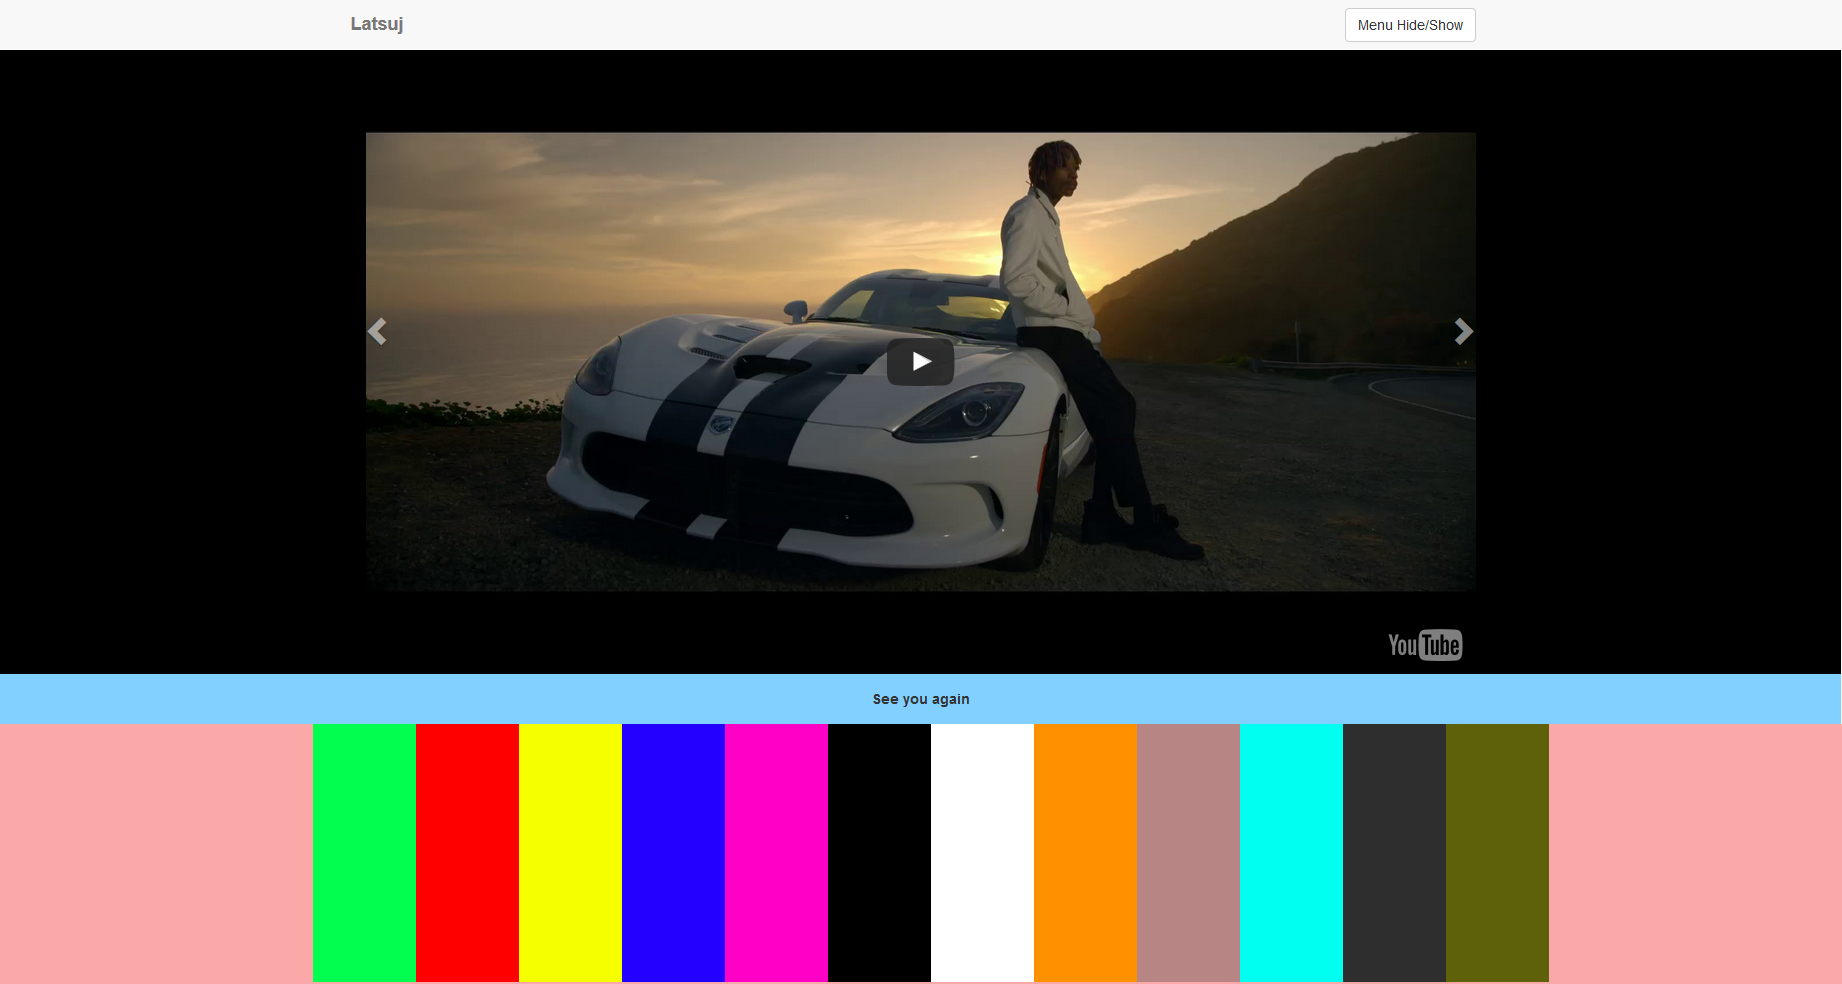
\includegraphics[width=0.48\textwidth]{p12}
  \end{center}
  \vspace{-20pt}
  \caption{Les 12 divisions d'un container}
  \vspace{-10pt}
\end{wrapfigure} 

Lorsque l'on utilise la classe \og row \fg{} dans Bootstrap, on divise ce container en 12 parties \'egales. Avec Polymer, le principe que j'ai d\'evelopp\'e est globalement le m\^eme cependant j'ai d\^u reconstruire ces divisions de A \`a Z via les m\'edia queries et les attributs CSS (en particulier : width). Sur la figure 10, j'ai repr\'esent\'e chacune des divisions d'une couleur diff\'erente. Ensuite, on peux d\'efinir combien de colonnes ou divisions pourra prendre un \'el\'ement. (voir les explications du chap\^itre pr\'ec\'edent).\\

\newpage
\begin{wrapfigure}{r}{0.5\textwidth}
  \vspace{-25pt}
  \begin{center}
    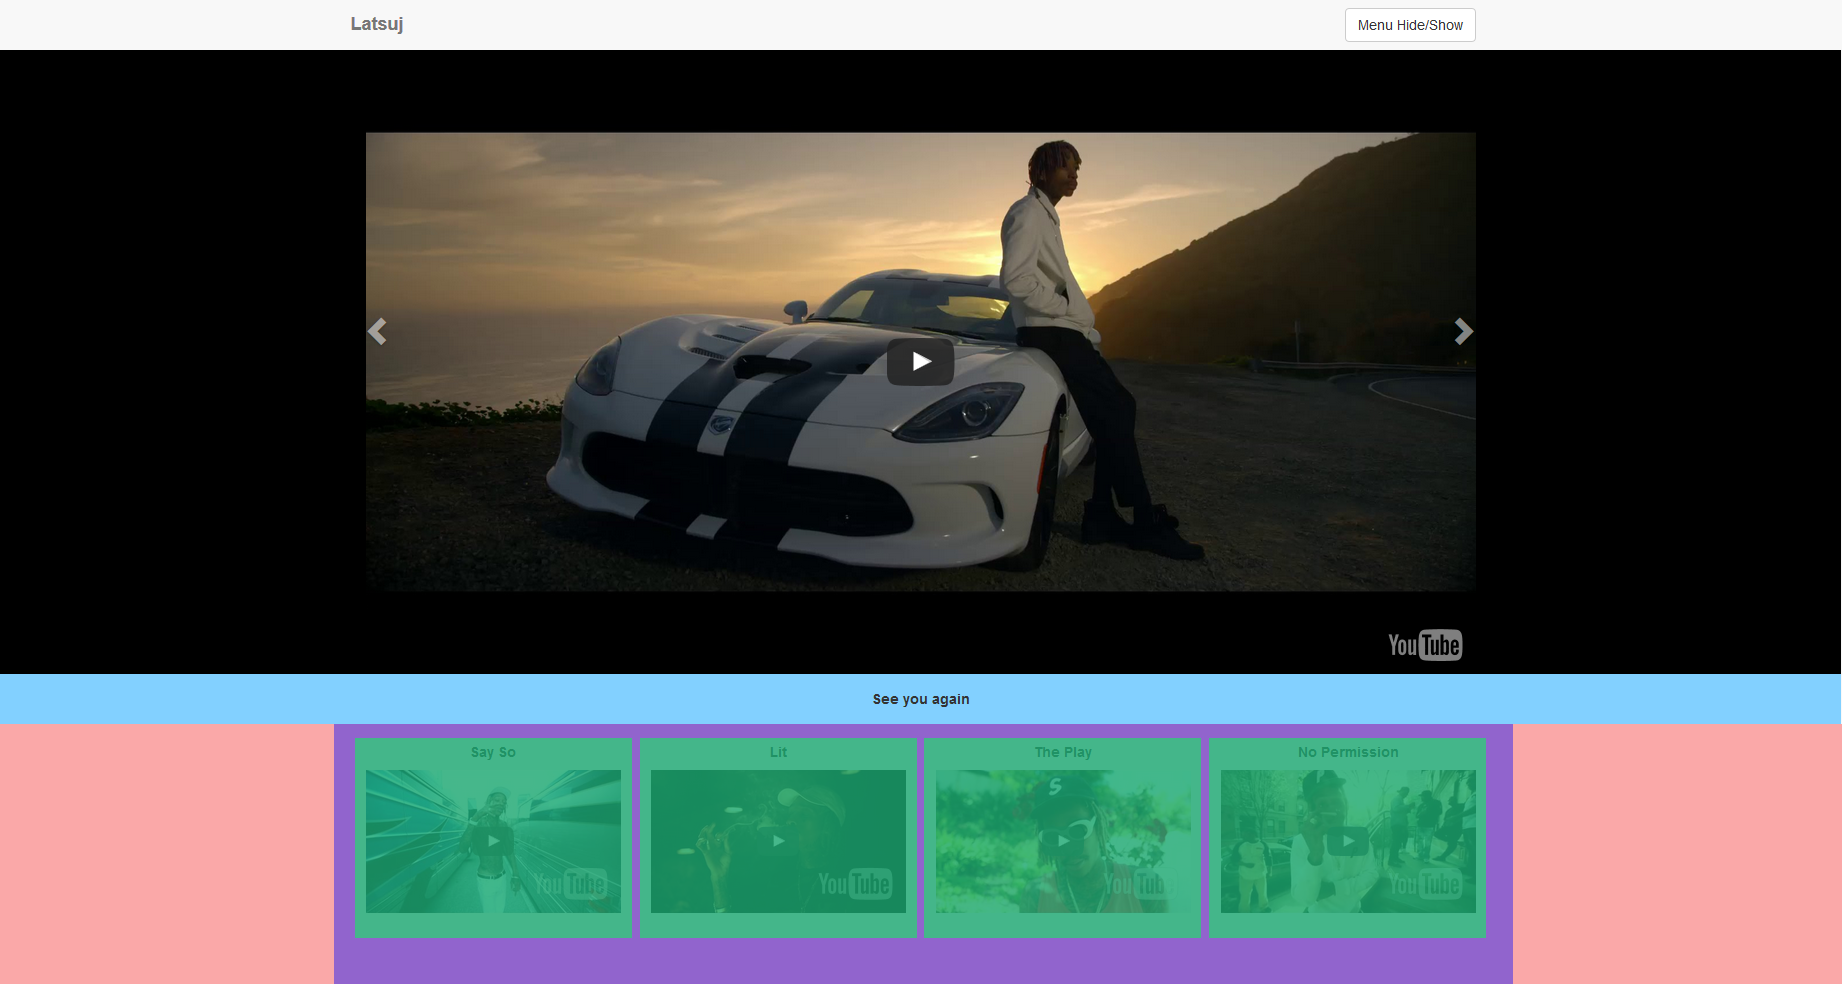
\includegraphics[width=0.48\textwidth]{p11}
  \end{center}
  \vspace{-20pt}
  \caption{Les 12 divisions d'un container}
  \vspace{-10pt}
\end{wrapfigure} 

Pour les clips musicaux en bas de page, j'ai d\'efini pour chacun d'entre eux 3 divisions. Sur Bootstrap, cela se traduit par \og col-XX-3 \fg{} o\`u XX repr\'esente tout simplement les points de rupture que j'ai \'evoqu\'e dans le chap\^itre pr\'ec\'edent. Avec Polymer, pour r\'ealiser cela, il faut imbriqu\'e deux modules ou balises l'une dans l'autre. La premi\`ere servira de container pour r\'ealiser la m\^eme chose que sur la figure 9 tandis que la deuxi\`eme servira \`a r\'ealiser les divisions comme sur l'image de droite.\\

Le point important est que les \'el\'ements des grille sont d\'efinis comme \og float:left \fg{} que ce soit sur Bootstrap ou sur Polymer. Ce qui veut dire qu'un \'el\'ement, ce positionnera toujours le plus \`a gauche possible sur la m\^eme ligne si il y a la place disponible, sinon l'\'el\'ement se positionnera sur une nouvelle ligne. De m\^eme, il y a toujours 12 colonnes sur une ligne peux importe la taille de la fen\^etre. Si jamais les \'el\'ements ex\'edent le nombre de colonnes disponibles sur la ligne, ils se placeronts automatiquement sur la ligne en dessous.\\

\begin{center}
\vspace{0.5cm}
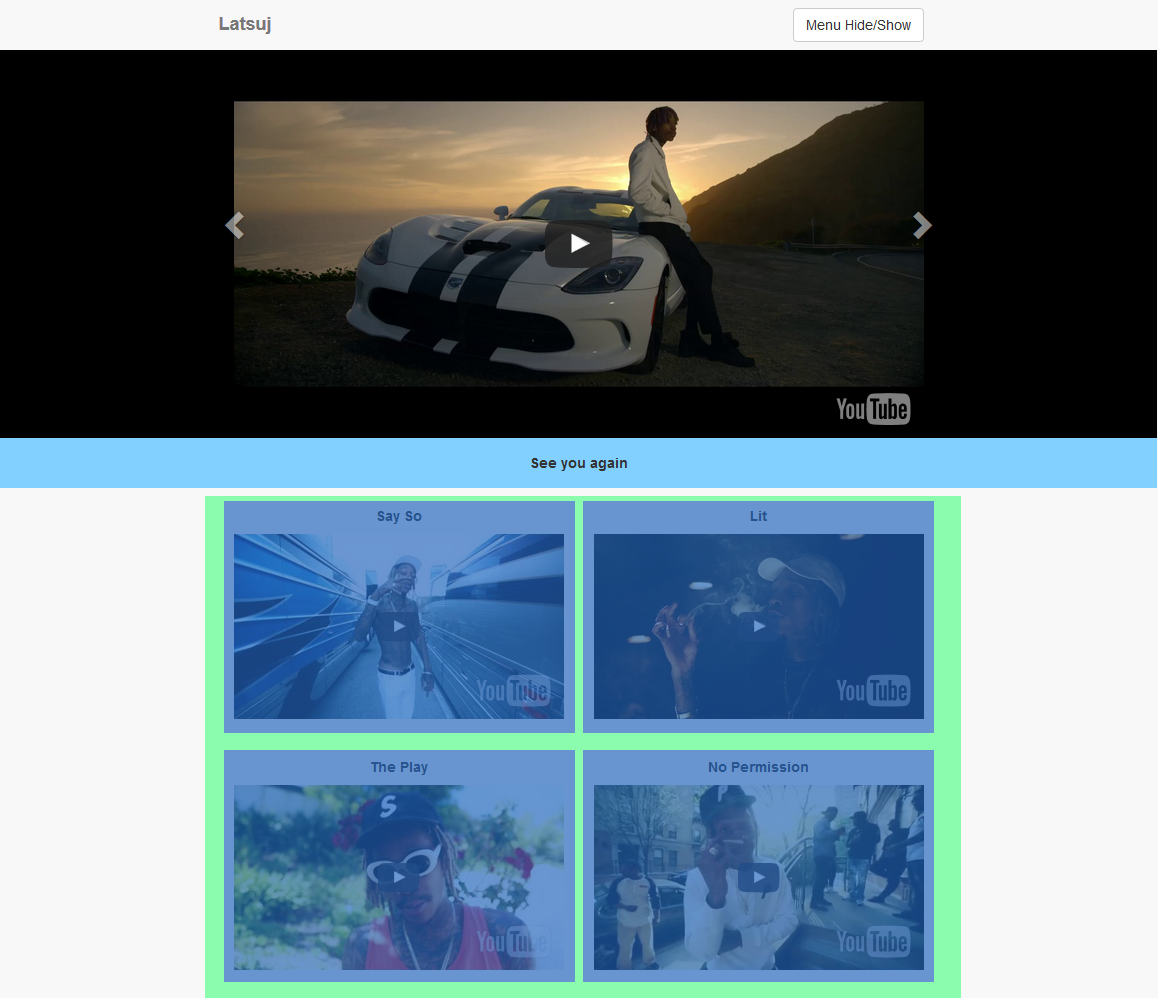
\includegraphics[width=0.8\textwidth]{p13}
\vspace{0.5cm}\\
\end{center}

Comme vu dans les exemples pr\'ec\'edent, les clips musicaux du bas de la page \'etaient affich\'es sur 1 ligne. Sur Bootstrap, cela \'equivaut \`a utiliser la classe \og col-XX-3 \fg{}. Il y a 4 vid\'eos qui utilisent chacune 3 divisions. Sur Polymer, on pr\'ecisera que le bloc utilise 25\% du container en CSS avec l'attribut \og width \fg{}. Maintenant sur l'image ci-dessus, il y a deux lignes. Chacune utilise un syst\`eme de 12 colonnes. La diff\'erence r\'eside simplement dans le nombre de colonnes qu'on a permis \`a l'\'el\'ement d'utiliser. Ici, j'ai utilis\'e la classe \og col-XX-6 \fg{} sur Bootstrap. Pour indiquer que chaque vid\'eos prendrait 6 colonnes. Comme il y a 4 clips, les deux premieres vid\'eos ont remplit la premi\`ere ligne puis la troisi\`eme vid\'eo est automatiquement pass\'ee \`a la ligne en dessous pour compl\'eter le container.\\

Ainsi, nous avons une id\'ee g\'en\'erale des moyens que j'ai utilis\'e pour faire mon site ainsi qu'une compr\'ehension pouss\'ee des techniques que je vais employ\'e pour comprendre comment j'ai form\'e mon site.

\newpage
\section{L'exemple de A \`a Z}

\subsection{Installation}

\begin{wrapfigure}{r}{0.3\textwidth}
  \vspace{-25pt}
  \begin{center}
    
\includegraphics[width=0.28\textwidth]{p25}
  \end{center}
  \vspace{-20pt}
  \caption{WAMP}
  \vspace{-10pt}
\end{wrapfigure} 
Avant m\^eme de commencer \`a d\'evelopper, il faut installer les outils n\'ecessaires pour d\'eployer et ex\'ecuter les exemples expliqu\'es ci-dessous. Dans un premier temps, il faut savoir que j'ai utilis\'e un peu de PHP dans mon exemple. Il faut donc commencer par installer un interpr\'eteur. Dans mon cas, j'ai choisi WAMP Serveur. L'installation est relativement ais\'ee et bien expliqu\'ee sur le site officiel du logiciel. La seule difficult\'e possible que vous rencontr\'erez sera li\'e au port 80. Certaines applications comme Skype utilisent ce port par d\'efaut, il faut donc le lib\'erer pour que Apache (un logiciel dans wamp) puisse s'en servir. \\
Une fois le logiciel install\'e et fonctionnant sans probl\`eme (icone vert), il faut remplir un peu la base de donn\'ee avec quelques informations pour que mon exemple ci-dessous puisse fonctionner sans probl\`eme. Ci-dessous figure la structure globale de la base de donnée (PhpMyAdmin dans wamp) :
\begin{center}
\vspace{0.5cm}
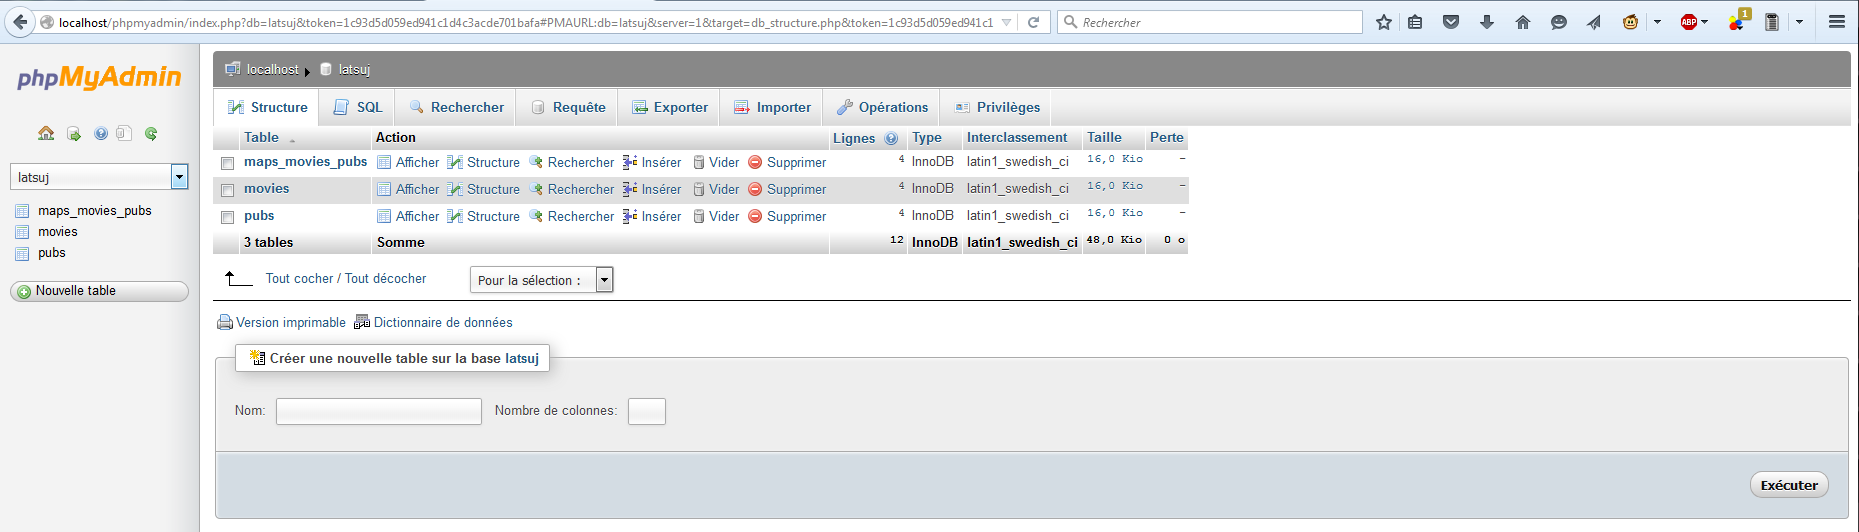
\includegraphics[width=\textwidth]{p26}
\vspace{0.5cm}\\
\end{center}
Pour plus de facilit\'e lors de la cr\'eation de la base de donn\'ee, il existe une fonction \`a ex\'ecuter dans le fichier sql.php qui se trouve dans inc qui se nomme : setup(). Cette fonction va automatiquement cr\'eer la base de donn\'ee suivant le sch\'ema que j'utiliserai ensuite. Il suffit alors de remplir la base \og latsuj \fg{}.  
\begin{center}
\vspace{0.5cm}
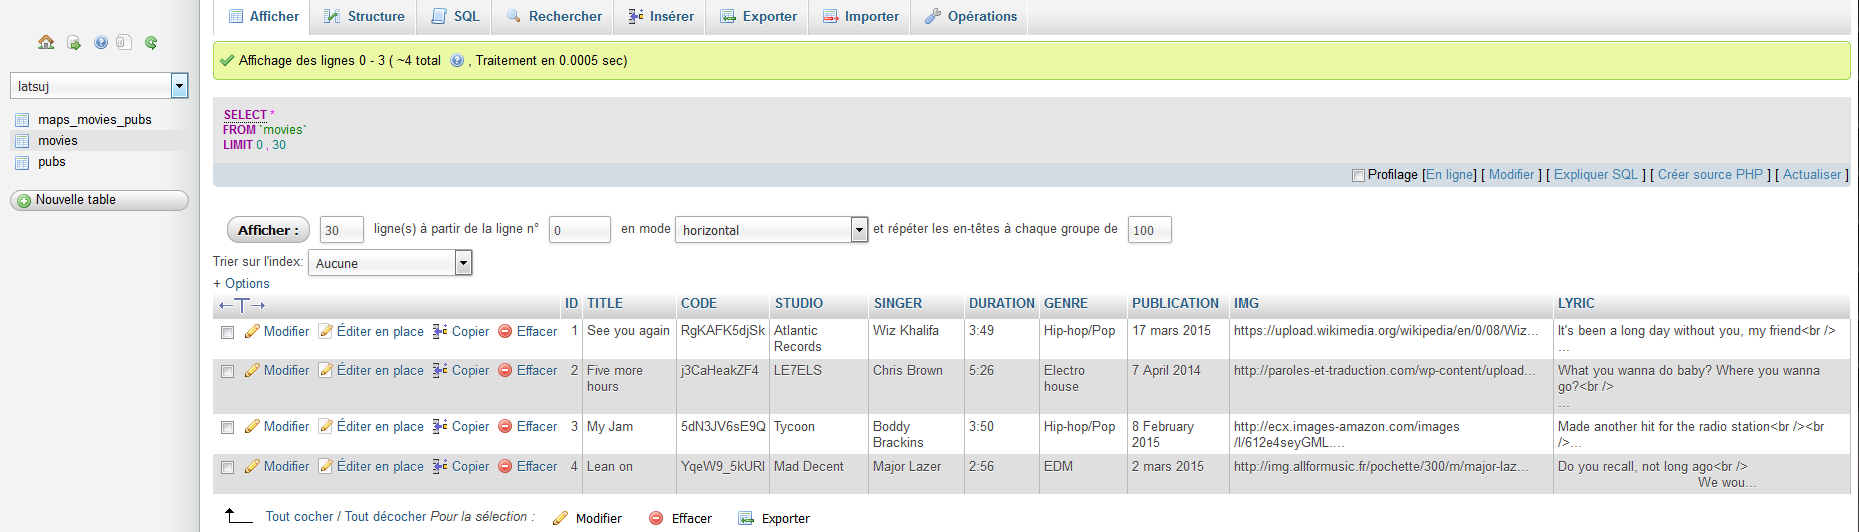
\includegraphics[width=\textwidth]{p27}
\vspace{0.5cm}\\
\end{center}
La table \og movie \fg{} permet de donner l'ensemble des informations sur une vid\'eo. \og TITLE \fg{} repr\'esente le titre de la musique. \og CODE \fg{} repr\'esente le code youtube du clip. \og STUDIO \fg{} repr\'esente le studio de d\'eveloppement de la musique. \og SINGER \fg{} repr\'esente le nom de l'artiste. \og DURATION \fg{} repr\'esente la dur\'ee exacte de la musique. \og GENRE \fg{} repr\'esente le genre de la musique. \og PUBLICATION \fg{} repr\'esente la date de la sortie de la musique. \og IMG \fg{} repr\'esente le lien de la jaquette de la musique. Et enfin \og LYRIC \fg{} repr\'esente les paroles de la musique.          
\begin{center}
\vspace{0.5cm}
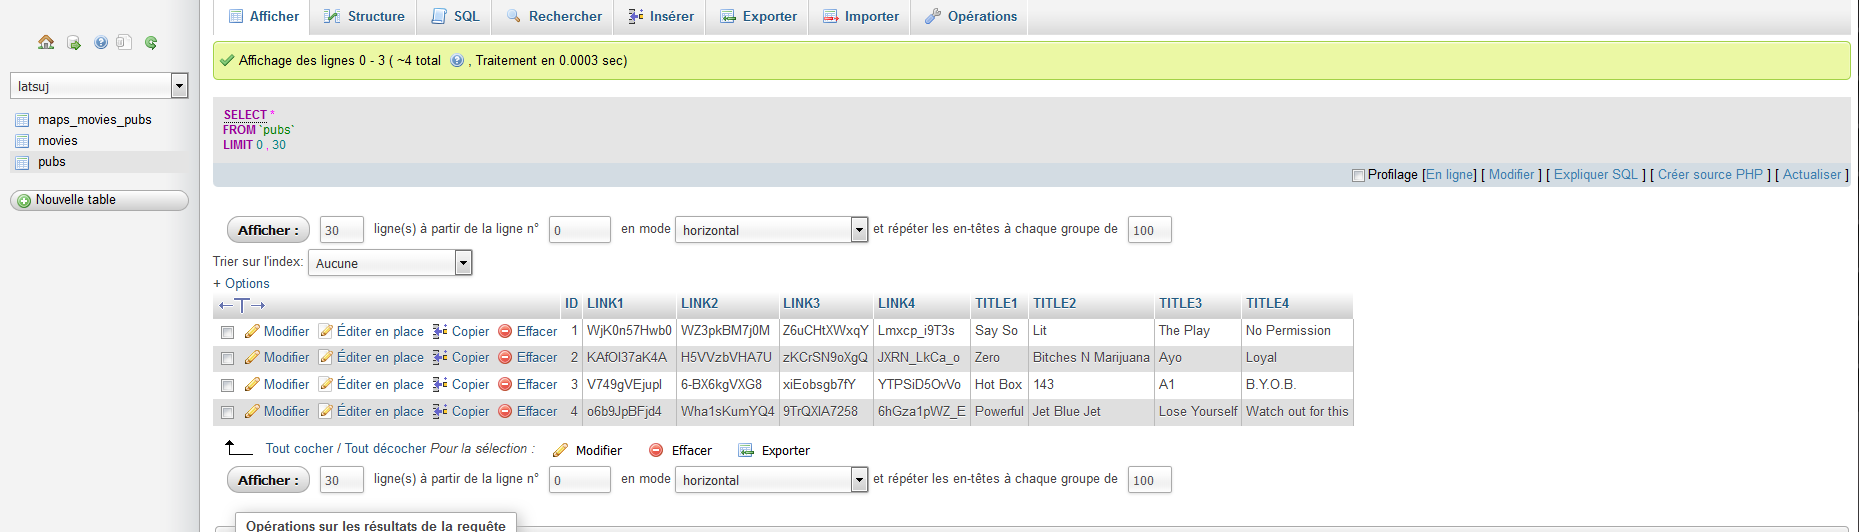
\includegraphics[width=\textwidth]{p28}
\vspace{0.5cm}\\
\end{center}
La table \og pubs \fg{} permet de sp\'ecifier les vid\'eos qui se trouvent en bas de page. Chaque colonne associe un lien avec un titre. Ainsi \og LINK1 \fg{} repr\'esente le lien youtube de la vid\'eo et \og TITLE1 \fg{} repr\'esente le titre de la vid\'eo. Et chacune des quatres vid\'eos suivent exactement le m\^eme principe.\\
Enfin la derni\`ere table n'est l\`a que pour r\'ealiser une association ONE-ONE d'une ID de la table \og movie \fg{} vers la table \og pubs \fg{}. Dans notre cas, il n'y a pas grand int\'er\^et ici car chaque id de "movie" sera attribu\'e a un id de "pub" qui sera au final identique. 1 va point\'e vers 1, 2 pointera vers 2...
\vspace{0.5cm}\\
Si vous souhaitez simplement lancer le site ou que vous disposez des fichiers, il faudra placer l'ensemble des fichiers du site dans le r\'epertoire "www" de wamp puis lancer un navigateur internet sur l'adresse suivante pour Boostrap par exemple : \textit{http://localhost/Bootstrap/index.php}.\\
Si vous souhaitez simplement suivre le tutoriel, il faudra dans chaque technologie effectu\'ee une installation suppl\'ementaire dans un fichier index.html \`a placer dans le repertoire "www" de WAMP. Pour Bootstrap, il faudra simplement rajouter les CDN dans le fichier, c'est \`a dire les fichiers CSS et JavaScript :
\vspace{0.5cm}\\
\fbox{\parbox{\textwidth}{
<link rel="stylesheet" href="https://maxcdn.bootstrapcdn.com/bootstrap/3.3.5/css/bootstrap.min. css">\\
<link rel="stylesheet" href="https://maxcdn.bootstrapcdn.com/bootstrap/3.3.5/css/bootstrap-theme.min.css">\\
<script src="https://maxcdn.bootstrapcdn.com/bootstrap/3.3.5/js/bootstrap.min.js"></script>
}}
\vspace{0.5cm}\\
Pour Polymer, c'est un petit peu plus complexe, il faudra install\'e Node.js puis suivre \`a la lettre toutes les commandes indiqu\'ees sur la page officielle de Polymer pour cr\'eer un projet Polymer.

\subsection{Creation des containers}

Il est maintenant temps de commencer l'application de ce que nous avons vu pr\'ec\'edent dans un exemple concret. Nous allons reproduire l'ensemble de mon site sous les deux technologies que sont Polymer et Bootstrap. Si vous avez compris ce que j'ai expliqu\'e dans le chap\^itre pr\'ec\'edent, il faut commencer par cr\'eer nos containers. C'est \`a dire nos \'el\'ements qui serviront de base \`a nos grilles de positionnement.

\begin{wrapfigure}{r}{0.5\textwidth}
  \vspace{-25pt}
  \begin{center}
    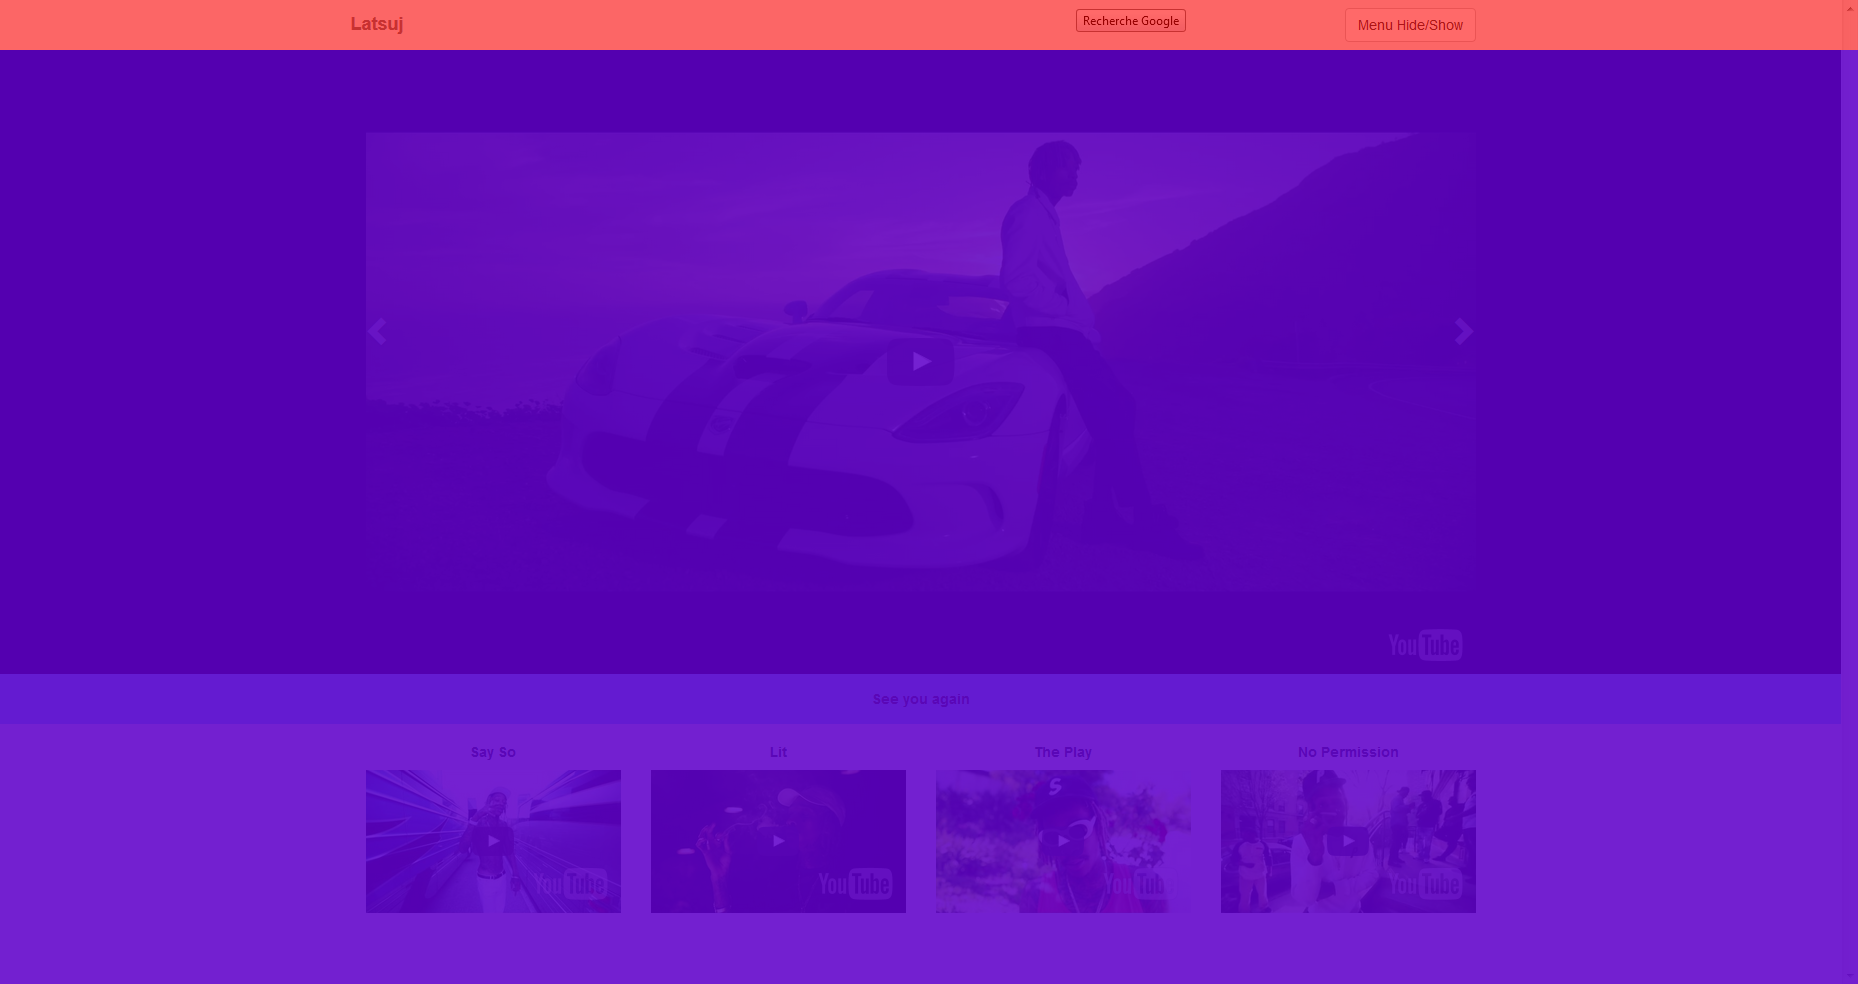
\includegraphics[width=0.48\textwidth]{p18}
  \end{center}
  \vspace{-20pt}
  \caption{Les 12 divisions d'un container}
  \vspace{-10pt}
\end{wrapfigure} 

Sur mon exemple, il y a deux grands blocs principaux. Un container ou plut\^ot une barre principale qui se trouve en haut du site (zone rouge sur l'image \`a droite) et une partie contenue qui est en fait un grand carrousel (couleur violette sur l'image \`a droite). La partie violette sera une partie du site qui sera anim\'ee via un script JQuery mais suivra globalement la m\^eme structure.\\

Sous Bootstrap, j'ai utilis\'e trois classes sur des balises HTML pour r\'ealiser cela facilement : \og container-fluid \fg{}, \og navbar \fg{} et \og container \fg{}. La premi\`ere permet de sp\'ecifier que nous utiliserons 100\% de la largeur de la fen\^etre. La seconde est la balise pour sp\'ecifier o\`u se trouve notre menu de navigation. La derni\`ere permet de prendre la dimension en pixel avant le point de rupture. Les autres classes qui se trouvent dans l'exemple ci-dessous ne sont que des classes am\'eliorant le design et ne sont donc pas n\'ec\'essaire pour reproduire mon exemple. Ainsi je n'expliquerais pas leurs utilit\'e, la plupart \'etant expliqu\'e dans la documentation de Bootstrap. 
\vspace{0.5cm}\\
\fbox{\parbox{\textwidth}{
...\\
<body>\\
\hspace*{0.6cm}<nav class="navbar navbar-default navbar-static-top">\\
\hspace*{1.2cm}<div class="container-fluid black">\\
\hspace*{1.2cm}</div>\\
\hspace*{0.6cm}</nav>\\
\hspace*{0.6cm}<div class="container-fluid black">\\
\hspace*{0.6cm}</div>\\
</body>\\
...
}}
\vspace{0.5cm}\\
Sous Polymer, nous allons simplement reproduire le comportement des classes pr\'ec\'edentes et en faire de nouveaux \'el\'ements   du DOM (Document Object Model). Pour faire cela proprement, j'ai utilis\'e Firebugs et a analys\'e le CSS utilis\'e sur Bootstrap pour reproduire le style de ces classes. Le code sous Polymer dans la page index est le suivant :
\vspace{0.5cm}\\
\fbox{\parbox{\textwidth}{
...\\
<body>\\
\hspace*{0.6cm}<bar-top>\\
\hspace*{1.2cm}<my-container>\\
\hspace*{1.2cm}</my-container>\\
\hspace*{0.6cm}</bar-top>\\
\hspace*{0.6cm}<my-container-full>\\
\hspace*{0.6cm}</my-container-full>\\
</body>\\
...
}}
\vspace{0.5cm}\\
Pour que ce code fonctionne correctement, il faut bien \'evidemment cr\'eer les modules. Un module est simplement une page HTML avec une certaine syntaxe que nous incorporons dans la page principale (index.html) avec le code suivant \`a placer entre les balises HEAD :
\vspace{0.5cm}\\
\fbox{\parbox{\textwidth}{
<link rel="import" href="bar-top.html">\\
<link rel="import" href="my-container.html">\\
<link rel="import" href="my-container-full.html">
}}
\vspace{0.5cm}\\

Le fichier bar-top.html qui repr\'esentera notre nouvelle \'el\'ement du DOM aura son style CSS fix\'e \`a lui. \`A noter que la syntaxe est extr\^emement importante. Un module doit obligatoirement \^etre nomm\'e de la fa\c{c}on suivante (xxxx-xxxx). Le code ci-dessous est \`a ajouter au m\^eme niveau que index.html dans le fichier \textbf{bar-top.html} :
\vspace{0.5cm}\\
\fbox{\parbox{\textwidth}{
<dom-module id="bar-top">\\
\hspace*{0.6cm}<template>\\
\hspace*{1.2cm}<style>\\
\hspace*{1.8cm}\color{red}{:host} \{	\\		
\hspace*{2.4cm}\color{black}{background-color: \#f8f8f8;\\
\hspace*{2.4cm}border-color: \#e7e7e7;\\
\hspace*{2.4cm}z-index: 1000;\\
\hspace*{2.4cm}border-width: 0 0 1px;\\
\hspace*{2.4cm}position: relative;\\
\hspace*{2.4cm}min-height: 50px;\\
\hspace*{2.4cm}display: block;\\
\hspace*{2.4cm}box-sizing: border-box;\\		
\hspace*{2.4cm}border: none;\\
\hspace*{1.8cm}\}		\\		
\hspace*{1.8cm}@media (min-width: 768px) \{\\
\hspace*{2.4cm}:host \{\\
\hspace*{3.0cm}border-radius: 0;\\
\hspace*{2.4cm}\}	\\	
\hspace*{1.8cm}\}\\
\hspace*{1.2cm}</style>}\\
\hspace*{1.2cm}\color{red}{<content></content>}\\		
\hspace*{0.6cm}\color{black}{</template>\\
\hspace*{0.6cm}<script>}\\
\hspace*{0.6cm}\color{red}{Polymer(\{\\
\hspace*{1.2cm}is: "bar-top"\\
\hspace*{0.6cm}\});}\\
\hspace*{0.6cm}\color{black}{</script>\\
</dom-module>}
}}
\vspace{0.5cm}\\
Comme dit plus haut, il s'agit du module \og bar-top \fg{}, le lien avec ce code est r\'ealiser avec l'id du dom-module ainsi que le script qui sp\'ecifie son nom. \og :host \fg{} repr\'esente le module lui-m\^eme. Toutes les r\`egles CSS inscritent dans ce tag prendra automatiquement effet pour tout \'el\'ement <bar-top></bar-top>. Enfin la balise \og content \fg{} est le point d'ancrage du nouvelle \'el\'ement. C'est \`a dire que le code se trouvant entre les balises <bar-top> et </bar-top> se positionnera \`a l'int\'erieur des balises \og content \fg{}. Pour les m\'edia queries, j'ai d\'ej\`a expliqu\'e leurs fonctionnements dans le chapitre pr\'ec\'edent.\\
Ainsi la cr\'eation de module prendra toujours la m\^eme forme, il faut reproduire l'op\'eration pour que les deux autres modules prennent eux aussi effet :   
\vspace{0.5cm}\\
\fbox{\parbox{\textwidth}{
<dom-module id="my-container">\\
\hspace*{0.6cm}<template>\\
\hspace*{1.2cm}<style>\\
\hspace*{1.8cm}:host \{\\
\hspace*{2.4cm}padding-right: 15px;\\
\hspace*{2.4cm}padding-left: 15px;\\
\hspace*{2.4cm}margin-right: auto;\\
\hspace*{2.4cm}margin-left: auto;\\
\hspace*{2.4cm}box-sizing: border-box;\\
\hspace*{2.4cm}display: block;\\
\hspace*{2.4cm}height: auto;\\
\hspace*{1.8cm}\}\\	
\hspace*{1.8cm}@media (min-width:900px) \{\\
\hspace*{2.4cm}:host \{\\
\hspace*{3.0cm}width:700px;\\
\hspace*{2.4cm}\}\\
\hspace*{1.8cm}\}\\
\hspace*{1.8cm}@media (min-width:1200px) \{\\
\hspace*{2.4cm}:host \{\\
\hspace*{3.0cm}width:970px;\\
\hspace*{2.4cm}\}\\
\hspace*{1.8cm}\}\\
\hspace*{1.8cm}@media (min-width:1500px) \{\\
\hspace*{2.4cm}:host \{\\
\hspace*{3.0cm}width:1170px;\\
\hspace*{2.4cm}\}\\
\hspace*{1.8cm}\}\\
\hspace*{1.2cm}</style>\\
\hspace*{1.2cm}<content></content>\\
\hspace*{0.6cm}</template>\\
\hspace*{0.6cm}<script>\\
\hspace*{0.6cm}Polymer(\{\\
\hspace*{1.2cm}is: "my-container"\\
\hspace*{0.6cm}\});\\
\hspace*{0.6cm}</script>\\
</dom-module>
}}
\vspace{0.5cm}\\
\fbox{\parbox{\textwidth}{
<dom-module id="my-container-full">\\
\hspace*{0.6cm}<template>\\
\hspace*{1.2cm}<style>	\\	
\hspace*{1.8cm}:host \{\\	
\hspace*{2.4cm}display: block;	\\
\hspace*{2.4cm}position: absolute;\\
\hspace*{2.4cm}width: 100\%;\\
\hspace*{2.4cm}height: auto;\\
\hspace*{1.8cm}\}\\
\hspace*{1.2cm}</style>\\
\hspace*{1.2cm}<content></content>\\
\hspace*{0.6cm}</template>\\
\hspace*{0.6cm}<script>\\
\hspace*{0.6cm}Polymer(\{\\
\hspace*{1.2cm}is: "my-container-full"\\
\hspace*{0.6cm}\});\\
\hspace*{0.6cm}</script>\\
</dom-module>
}}
\vspace{0.5cm}\\
Ainsi nous obtenons le m\^eme r\'esultat avec les deux technologies. Nos containers \'etant maintenant pr\^et, nous allons nous occuper de la barre du haut (zone rouge dans la figure 12).

\subsection{Barre de menu}

\begin{center}
\vspace{0.5cm}

\includegraphics[width=\textwidth]{p19}
\end{center}

Le menu est compos\'e de ma signature \og Latsuj \fg{}, tout simplement mon nom \`a l'envers ainsi qu'un bouton pour afficher ou cacher le menu. J'ai choisi de mettre ma signature \`a gauche \`a cause de la nature de l'utilisateur. Un humain lit toujours de mani`ere inconsciente en diagonale. C'est aussi ce que l'on nomme lecture-rapide. Le premier mot que l'utilisateur verra sera donc ma signature. Ensuite, j'ai mis le bouton \`a droite pour faire \'echo au texte \`a gauche, la nature pr\'ef\`ere ce qui est sym\'etrique, ainsi que pour utiliser toutes la place disponible. Sous Bootstrap, comme toujours nous avons des classes pour r\'ealiser cela sans trop se fatiguer. Par rapport \`a ce dont j'ai parl\'e pr\'ec\'edemment, il y aura 3 nouvelles classes ici que je n'ai pas encore \'evoqu\'e : \og pull-left \fg{},\og pull-right \fg{}, \og btn \fg{}. Les deux classes \og pull \fg{} permettent de pousser leurs contenus vers la gauche ou la droite. \og Btn \fg{} permet quant \`a elle de mettre le style d'un bouton sur le composant o\`u on l'utilise. On obtient alors notre menu assez facilement :
\vspace{0.5cm}\\
\fbox{\parbox{\textwidth}{
\hspace*{0.6cm}<nav class="navbar navbar-default navbar-static-top">\\
\hspace*{1.2cm}<div class="container"> 	\\
\hspace*{1.8cm}<div class="row">\\   
\hspace*{2.4cm}<div class="col-sm-12 col-md-12 col-lg-12">\\
\hspace*{3.0cm}<div class="pull-left">\\
\hspace*{3.6cm}<strong class="navbar-brand">Latsuj</strong>\\
\hspace*{3.0cm}</div>\\
\hspace*{3.0cm}<div class="pull-right navbar-brand">\\
\hspace*{3.6cm}<div class="menu-toggle btn btn-default">Menu Hide/Show</div>\\
\hspace*{3.0cm}</div>\\
\hspace*{2.4cm}</div>\\
\hspace*{1.8cm}</div>\\
\hspace*{1.2cm}</div>\\
\hspace*{0.6cm}</nav>
}}
\vspace{0.5cm}\\
A noter ici que nous aurions pu sp\'ecifier que notre signature prenne 2 colonnes, que le bouton prenne aussi 2 colonnes et mettre un offset entre les deux de 8 colonnes. Cependant, j'ai pr\'ef\'er\'e cette m\'ethode car cela me fait moins de ligne de code donc un code plus clair. Les classes dont je n'explique pas le r\^ole ne sont l\`a que pour rendre les choses plus jolie et ne sont pas n\'eccesaire pour reproduire l'architecture de mon site/exemple. Avec le simple exemple ci-dessus, nous obtenons sous Bootstrap notre menu. Sous Polymer, il va falloir comme pr\'ec\'edemment reproduire le comportement des blocs de Bootstrap en cr\'eant de nouvelles nodes. Dans le code qui va suivre, il n'y a rien de nouveau, ni de compliqu\'e, ce n'est que du CSS :
\vspace{0.5cm}\\
\fbox{\parbox{\textwidth}{
<dom-module id="my-row">\\
\hspace*{0.6cm}<template>\\
\hspace*{1.2cm}<style>	\\	
\hspace*{1.8cm}:host \{\\
\hspace*{2.4cm}display: block;\\
\hspace*{2.4cm}position: relative;\\
\hspace*{2.4cm}margin-right: -15px;\\
\hspace*{2.4cm}margin-left: -15px;\\
\hspace*{2.4cm}box-sizing: border-box;\\
\hspace*{1.8cm}\}\\
\hspace*{1.2cm}</style>\\
\hspace*{1.2cm}<content></content>\\
\hspace*{0.6cm}</template>\\
\hspace*{0.6cm}<script>\\
\hspace*{1.2cm}Polymer(\{\\
\hspace*{1.8cm}is: "my-row"\\
\hspace*{1.2cm}\});\\
\hspace*{0.6cm}</script>\\
</dom-module>
}}
\vspace{0.5cm}

Il n'y a rien de particulier sur ce module \og my-row \fg{} qui reproduit le comportement de la classe \og row \fg{} de Boostrap. Notons cependant que dans Polymer, les nouveaux modules sont toujours sp\'ecifi\'e comme \og display:inline \fg{}, il faut donc tr\`es souvent les passer en \og display:bloc \fg{}. Notons par ailleurs l'utilisation de box-sizing qui n'est peut-\^etre pas n\'ecessaire ici. Ayant voulu cr\'eer un site fonctionnant sur tous les navigateurs, cet attribut est essentiel. Cependant, Polymer \'etant tr\`es mal support\'e pour l'instant, cet attribut perd de son int\'er\^et au jour d'aujourd'hui. Si les navigateurs s'effor\c{c}aient de faire le n\'ecessaire pour supporter Polymer, il n'y aurait pas besoin de modifier mon exemple car j'aurais d\'ej\`a pr\'evu cela.
\vspace{0.5cm}\\
\fbox{\parbox{\textwidth}{
<dom-module id="col-top">\\
\hspace*{0.6cm}<template>\\
\hspace*{1.2cm}<style>\\
\hspace*{1.8cm}:host \{\\
\hspace*{2.4cm}display: block;\\
\hspace*{2.4cm}position: relative;\\
\hspace*{2.4cm}padding-right: 15px;\\
\hspace*{2.4cm}padding-left: 15px;\\
\hspace*{2.4cm}box-sizing: border-box;\\
\hspace*{2.4cm}min-height: 50px; \\  
\hspace*{2.4cm}float: left;\\
\hspace*{2.4cm}width: 100\%;\\
\hspace*{1.8cm}\}\\
\hspace*{1.8cm}</style>\\
\hspace*{1.8cm}<content></content>\\
\hspace*{1.2cm}</template>\\
\hspace*{1.2cm}<script>\\
\hspace*{1.2cm}Polymer(\{\\
\hspace*{1.8cm}is: "col-top"\\
\hspace*{1.2cm}\});\\
\hspace*{0.6cm}</script>\\
</dom-module>
}}
\vspace{0.5cm}

Ce module \og col-top \fg{} reprend la d\'efinition de la classe \og col \fg{} de Bootstrap. Il n'y a rien de sp\'ecial dans ce module, l'ensemble de ces attributs on d\'ej\`a \'et\'e comment\'e.  
\vspace{0.5cm}\\
\fbox{\parbox{0.5\textwidth}{
<dom-module id="pull-left">\\
\hspace*{0.6cm}<template>\\
\hspace*{1.2cm}<style>\\
\hspace*{1.8cm}:host \{\\
\hspace*{2.4cm}display: block;\\
\hspace*{2.4cm}float: left!important;\\
\hspace*{2.4cm}box-sizing: border-box;\\
\hspace*{2.4cm}margin-left: -15px;\\  		
\hspace*{2.4cm}min-height: 50px;\\
\hspace*{2.4cm}padding: 15px 15px;\\
\hspace*{2.4cm}font-size: 18px;\\
\hspace*{2.4cm}line-height: 40px;\\
\hspace*{2.4cm}margin-top: -15px;\\
\hspace*{1.8cm}\}\\
\hspace*{1.8cm}</style>	\\
\hspace*{1.8cm}<content></content> 	\\
\hspace*{1.2cm}</template>\\
\hspace*{1.2cm}<script>\\
\hspace*{1.2cm}Polymer(\{\\
\hspace*{1.8cm}is: "pull-left"\\
\hspace*{1.2cm}\});\\
\hspace*{0.6cm}</script>\\
</dom-module>
}}
\fbox{\parbox{0.5\textwidth}{
<dom-module id="pull-right">\\
\hspace*{0.6cm}<template>\\
\hspace*{1.2cm}<style>\\
\hspace*{1.8cm}:host \{\\
\hspace*{2.4cm}display: block;\\
\hspace*{2.4cm}float: right!important;\\
\hspace*{2.4cm}box-sizing: border-box;\\
\hspace*{2.4cm}margin-left: -15px;\\  		
\hspace*{2.4cm}min-height: 50px;\\
\hspace*{2.4cm}padding: 15px 15px;\\
\hspace*{2.4cm}font-size: 18px;\\
\hspace*{2.4cm}line-height: 40px;\\
\hspace*{2.4cm}margin-top: -15px;\\
\hspace*{1.8cm}\}\\
\hspace*{1.8cm}</style>	\\
\hspace*{1.8cm}<content></content> 	\\
\hspace*{1.2cm}</template>\\
\hspace*{1.2cm}<script>\\
\hspace*{1.2cm}Polymer(\{\\
\hspace*{1.8cm}is: "pull-right"\\
\hspace*{1.2cm}\});\\
\hspace*{0.6cm}</script>\\
</dom-module>
}}
\vspace{0.5cm} 
  
Ces deux modules servent \`a aligner leurs contenues \`a droite ou \`a gauche dans leurs containers. Pour des raisons graphiques, j'ai ajout\'e un attribut \og margin-top \fg{}. La seule diff\'erence entre ces deux blocs r\'eside dans leur float. On aurais pu cr\'eer un seul \'el\'ement et sp\'ecifier ensuite dans le fichier index.html un style particulier vers la gauche ou la droite. Cependant, j'ai trouv\'e plus int\'err\'essant de s\'eparer tout l'aspect graphique de l'index et des modules. Polymer proscrit l'emploie de feuille de style s\'epar\'e pour la page HTML qui sera affich\'e. Les r\`egles CSS se trouve soit dans le module ou alors dans une balise style d\'efini \og is="custom-style" \fg{}.  
\vspace{0.5cm}\\
\fbox{\parbox{\textwidth}{
<dom-module id="title-top">\\
\hspace*{0.6cm}<template>\\
\hspace*{1.2cm}<style>\\
\hspace*{1.8cm}:host \{ \\   
\hspace*{2.4cm}margin-left:-15px;\\
\hspace*{2.4cm}line-height: 40px;\\
\hspace*{2.4cm}float: left;\\
\hspace*{2.4cm}height: 50px;\\
\hspace*{2.4cm}padding: 15px 15px;\\
\hspace*{2.4cm}font-size: 18px;\\
\hspace*{2.4cm}margin-top: -12px;	\\	
\hspace*{2.4cm}color:\#777;\\
\hspace*{1.8cm}\}	  	\\			  	
\hspace*{1.8cm}b,strong \{\\
\hspace*{2.4cm}font-weight:700;\\
\hspace*{1.8cm}\}\\
\hspace*{1.2cm}</style>\\
\hspace*{1.8cm}<strong>Latsuj</strong>\\ 	
\hspace*{1.2cm}</template>\\
\hspace*{1.2cm}<script>\\
\hspace*{1.2cm}Polymer(\{\\
\hspace*{1.8cm}is: "title-top"\\
\hspace*{1.2cm}\});\\
\hspace*{0.6cm}</script>\\
</dom-module>
}}
\vspace{0.5cm}\\
Le module \og title-top \fg{} est le module qui permet d'afficher le titre. J'ai pr\'ef\'er\'e l\`a aussi en faire un module car cela permet de bien d\'ecouper mon code. Je sais o\`u se trouve toutes les r\`egles CSS en rapport avec ce dernier. 
\vspace{0.5cm}\\
\fbox{\parbox{\textwidth}{
<dom-module id="my-button">\\
\hspace*{0.6cm}<template>\\
\hspace*{1.2cm}<style>	\\	
\hspace*{1.8cm}:host \{	\\
\hspace*{2.4cm}color: \#333;\\
\hspace*{2.4cm}background-color: \#FFF;\\
\hspace*{2.4cm}display: inline-block;\\
\hspace*{2.4cm}margin-bottom: 0px;\\
\hspace*{2.4cm}font-weight: normal;\\
\hspace*{2.4cm}text-align: center;\\
\hspace*{2.4cm}vertical-align: middle;\\
\hspace*{2.4cm}cursor: pointer;\\
\hspace*{2.4cm}background-image: none;\\
\hspace*{2.4cm}border: 1px solid \#CCC;\\
\hspace*{2.4cm}white-space: nowrap;\\
\hspace*{2.4cm}padding: 6px 12px;\\
\hspace*{2.4cm}font-size: 14px;\\
\hspace*{2.4cm}line-height: 1.42857;\\
\hspace*{2.4cm}border-radius: 4px;\\
}}
\fbox{\parbox{\textwidth}{
\hspace*{2.4cm}-moz-user-select: none;\\
\hspace*{2.4cm}box-sizing: border-box;\\
\hspace*{1.8cm}\}\\
\hspace*{1.8cm}:host(:focus)\{\\
\hspace*{2.4cm}color: \#333;\\
\hspace*{2.4cm}background-color: \#E6E6E6;\\
\hspace*{2.4cm}border-color: \#8C8C8C;	\\	
\hspace*{1.8cm}\}	\\	
\hspace*{1.8cm}:host(:active) \{\\
\hspace*{2.4cm}color: \#333;\\
\hspace*{2.4cm}background-color: \#D4D4D4;\\
\hspace*{2.4cm}border-color: \#8C8C8C;\\
\hspace*{2.4cm}outline: 0px none;\\
\hspace*{2.4cm}background-image: none;\\
\hspace*{2.4cm}box-shadow: 0px 3px 5px rgba(0, 0, 0, 0.125) inset;\\
\hspace*{1.8cm}\}\\
\hspace*{1.2cm}</style>\\
\hspace*{1.8cm}<div>Menu Hide/Show</div>\\
\hspace*{1.2cm}</template>\\
\hspace*{1.2cm}<script>\\
\hspace*{1.2cm}Polymer(\{\\
\hspace*{1.8cm}is: "my-button"\\
\hspace*{1.2cm}\});\\
\hspace*{0.6cm}</script>\\
</dom-module>
}}
\vspace{0.5cm}\\
Ce gros module est celui qui va repr\'senter notre bouton en haut \`a droite. Je vais m'attarder sur une petite particularit\'e. Dans le code, on retrouve deux blocs de r\`egles qui sont li\'e \`a des \'ev\`enements. Le premier \og :focus \fg{} permet de d\'efinir des r\`egles CSS lorsque le bouton aura le focus dans la fen\^etre. Le deuxi\`eme est un \'ev\`enement lorsque le bouton a \'et\'e cliqu\'e. On aurait pu aussi d\'efinir ces changements de r\`egles avec JavaScript mais j'ai choisi d'accomplir cela comme il est indiqu\'e dans la documentation de Polymer. 
\vspace{0.5cm}\\
Nos modules \'etant cr\'e\'e, nous pouvons maintenant nous en servir pour reproduire le menu comme sur Bootstrap. Le code obtenu apr\`es tous ces efforts est simple et clair :
\vspace{0.5cm}\\
\fbox{\parbox{\textwidth}{
<bar-top>\\
\hspace*{0.6cm}<my-container>\\
\hspace*{1.2cm}<my-row>\\
\hspace*{1.8cm}<col-top>\\
\hspace*{2.4cm}<pull-left>\\
\hspace*{3.0cm}<title-top></title-top>\\
\hspace*{2.4cm}</pull-left>\\
\hspace*{2.4cm}<pull-right>\\
\hspace*{3.0cm}<my-button></my-button>\\
\hspace*{2.4cm}</pull-right>\\
\hspace*{1.8cm}</col-top>\\
\hspace*{1.2cm}</my-row>\\
\hspace*{0.6cm}</my-container>\\
</bar-top>
}}
\subsection{Le carousel}

Le carousel est la partie qui m'a demand\'e le plus de temps sous Polymer car rien n'a \'et\'e mis en place dans ce framework (structure logicielle). D'un autre cot\'e, Bootstrap a mis en place plusieurs classes pour avoir du contenu anim\'e facile \`a impl\'ement\'e. Le carousel est une de ces animations. Sous Bootstrap, 3 classes sont n\'ecessaire pour faire un carousel digne de ce nom : \og carousel \fg{}, \og carousel-inner \fg{} et \og item \fg{}. La premi\`ere classe permet d'initialiser le carousel et permet si il y a plusieurs carousels de faire la distinction entre ces derniers en sp\'ecifiant un ID. La deuxi\`eme classe d\'efinie la zone pour la page actuelle du carousel. Enfin, la derni\`ere classe permet de d\'efinir une slide du carousel. Pourquoi avoir choisi le carousel ? Tout simplement car il s'agit d'une m\'ethode d'animation simple et facile \`a comprendre. Elle permet d'avoir tout le contenu du site sur une page. Cependant, cela peut amener un probl\`eme qui d'ailleurs se trouve dans mon exemple. Lors du chargement de la premi\`ere page, on remarque que le site est relativement long \`a se charger. C'est tout simplement car mon site charge en fait l'ensemble des slides au chargement de la premi\`ere slide. On pourrait faire comme sur facebook et ne charger qu'une partie du contenu. Cependant, cela veut aussi dire que l'utilisateur devra charger toutes les X slides, les prochaines slides. Il y a donc un compromis \`a prendre. J'ai pr\'ef\'er\'e sur mon exemple, au vu du nombre faible de slide sur le site, faire que l'utilisateur charge l'ensemble des slides. Ainsi il ne souffre d'aucun ralentissement pendant l'utilisation.
\vspace{0.5cm}\\
\fbox{\parbox{\textwidth}{
<div class="container-fluid black">\\
\hspace*{0.6cm}<div id="myCarousel" class="carousel slide" data-ride="carousel" data-interval="false">\\
\hspace*{1.2cm}<div class="carousel-inner" role="listbox">\\
\hspace*{1.8cm}<div class="item active" >\\
\hspace*{2.4cm}...\\
\hspace*{1.8cm}</div>\\
\hspace*{1.8cm}<div class="item" >\\
\hspace*{2.4cm}...\\
\hspace*{1.8cm}</div>\\
\hspace*{1.2cm}</div>\\
\hspace*{0.6cm}</div>\\
</div>
}}	
\vspace{0.5cm}\\ 
L'attribut \og data-ride \fg{} permet de marquer le carousel comme anim\'e au chargement de la page. L'attribut \og data-interval \fg{} quant \`a lui renseigne sur le temps avant qu'une slide change \`a la suivante automatiquement. Enfin la classe \og active \fg{} indique simplement que le contenu de la div sera la premi\`ere slide du carousel.\\
Sous Polymer, c'est bien plus compliqu\'e pour fabriquer notre carousel. Pour arriver \`a faire cela, je me suis tout simplement bas\'e sur du JavaScript. Le fonctionnement est assez simple, toutes les slides sont positionn\'e \`a gauche de la fen\^etre sauf une qui sera affich\'e sur l'\'ecran de l'utilisateur. Lorsque l'on clique sur une fl\`eche vers la gauche ou la droite, la slide suivante se placera respectivement \`a droite ou \`a gauche de la slide courante. Enfin, on d\'eplace vers la gauche ou la droite, la slide courante et la slide suivante pour remplac\'e la slide actuelle par la suivante. Il n'y avait aucun moyen fournis dans Polymer pour effectuer cela autrement qu'en utilisant JavaScript.\\
Dans un premier temps, il faut cr\'eer les nouvelles nodes qui nous permettrons de faire le changement de slide. C'est \`a dire les fl\`eches sur la gauche et la droite de la vid\'eo principale.
\vspace{0.5cm}\\
\fbox{\parbox{0.5\textwidth}{
<dom-module id="my-right">\\
\hspace*{0.6cm}<template>\\
\hspace*{1.2cm}<style>	\\
\hspace*{1.8cm}img \{\\		
\hspace*{2.4cm}position:absolute;\\
\hspace*{2.4cm}right:1\%;\\
\hspace*{2.4cm}top:0;\\
\hspace*{2.4cm}bottom:0;\\
\hspace*{2.4cm}margin:auto;\\
\hspace*{2.4cm}z-index:1000;\\
\hspace*{2.4cm}opacity: 0.4;\\
\hspace*{2.4cm}transform:scale(1.1,1.1);\\
\hspace*{2.4cm}cursor:pointer;\\
\hspace*{1.8cm}\}	\\
\hspace*{1.8cm}img:hover \{\\
\hspace*{2.4cm}opacity: 1;\\
\hspace*{1.8cm}\}\\	
\hspace*{1.2cm}</style>\\
\hspace*{1.2cm}<img src="rightw.png"></img>\\
\hspace*{0.6cm}</template>\\
\hspace*{0.6cm}<script>\\
\hspace*{0.6cm}Polymer(\{\\
\hspace*{1.2cm}is: "my-right"\\
\hspace*{0.6cm}\});\\
\hspace*{0.6cm}</script>\\
</dom-module>
}}	
\fbox{\parbox{0.5\textwidth}{
<dom-module id="my-left">\\
\hspace*{0.6cm}<template>\\
\hspace*{1.2cm}<style>	\\
\hspace*{1.8cm}img \{\\		
\hspace*{2.4cm}position:absolute;\\
\hspace*{2.4cm}left:1\%;\\
\hspace*{2.4cm}top:0;\\
\hspace*{2.4cm}bottom:0;\\
\hspace*{2.4cm}margin:auto;\\
\hspace*{2.4cm}z-index:1000;\\
\hspace*{2.4cm}opacity: 0.4;\\
\hspace*{2.4cm}transform:scale(1.1,1.1);\\
\hspace*{2.4cm}cursor:pointer;\\
\hspace*{1.8cm}\}	\\
\hspace*{1.8cm}img:hover \{\\
\hspace*{2.4cm}opacity: 1;\\
\hspace*{1.8cm}\}\\	
\hspace*{1.2cm}</style>\\
\hspace*{1.2cm}<img src="rightw.png"></img>\\
\hspace*{0.6cm}</template>\\
\hspace*{0.6cm}<script>\\
\hspace*{0.6cm}Polymer(\{\\
\hspace*{1.2cm}is: "my-left"\\
\hspace*{0.6cm}\});\\
\hspace*{0.6cm}</script>\\
</dom-module>
}}	
\vspace{0.5cm}\\ 
On mettra ces \'el\'ements dans chacune des slides. Le code global de la page devient alors celui la :
\vspace{0.5cm}\\
\fbox{\parbox{\textwidth}{
...\\
<body>\\
\hspace*{0.6cm}<bar-top>\\
\hspace*{1.2cm}<my-container>\\
\hspace*{1.2cm}</my-container>\\
\hspace*{0.6cm}</bar-top>\\
\hspace*{0.6cm}<my-container-full id="XX">\\
\hspace*{1.2cm}<my-container>\\
\hspace*{1.8cm}<my-row>\\
\hspace*{2.4cm}<col-mid>\\
\hspace*{3.0cm}<my-left></my-left>\\
\hspace*{3.0cm}<my-right></my-right>\\
\hspace*{2.4cm}</col-mid>\\
\hspace*{1.8cm}</my-row>\\
\hspace*{1.2cm}</my-container>\\
\hspace*{0.6cm}</my-container-full>\\
</body>\\
...
}}
\vspace{0.5cm}\\

Le \og container-full \fg{} a comme on peux le voir un ID. Ce module repr\'esente une slide. Avec un peu de code PHP (car j'aime pas la duplication de code), je reproduis ce morceau de code plusieurs fois en incr\'ementant l'ID de 1. Cela permet d'identifier les slides facilement dans le script JavaScript qui est dessous : 
\vspace{0.5cm}\\
\fbox{\parbox{\textwidth}{
var slide=1;\\
var SLIDE\_MAX=4;\\
var SLIDE\_MIN=1;\\
\$("my-left").click(function() \{\\
\hspace*{0.6cm}\$("\#"+slide).css("right","0px");\\
\hspace*{0.6cm}\$("\#"+slide).animate(\{right: -\$(window).width()+"px"\},500);\\
\hspace*{0.6cm}slide++;\\
\hspace*{0.6cm}nextslide();\\
\hspace*{0.6cm}\$("\#"+slide).css("left","auto");\\
\hspace*{0.6cm}\$("\#"+slide).css("right",\$(window).width()+"px");\\
\hspace*{0.6cm}\$("\#"+slide).animate(\{right: \$("my-menu").width()+"px"\},350,function() \{\\
\hspace*{1.2cm}\$("\#"+slide).css("right","auto");\\	
\hspace*{0.6cm}\});\\
\});\\
\$("my-right").click(function() \{\\
\hspace*{0.6cm}\$("\#"+slide).css("left","0px");\\
\hspace*{0.6cm}\$("\#"+slide).animate(\{left: -\$(window).width()+"px"\},500);\\
\hspace*{0.6cm}slide--;\\
\hspace*{0.6cm}nextslide();\\
\hspace*{0.6cm}\$("\#"+slide).css("right","auto");\\
\hspace*{0.6cm}\$("\#"+slide).css("left",\$(window).width()+"px");\\
\hspace*{0.6cm}\$("\#"+slide).animate(\{left: \$("my-menu").width()+"px"\},350,function() \{\\
\hspace*{1.2cm}\$("\#"+slide).css("left","auto");\\
\hspace*{0.6cm}\});		\\
\});\\
function nextslide() \{\\
\hspace*{0.6cm}if(slide<1) \{\\
\hspace*{1.2cm}slide=SLIDE\_MAX;\\
\hspace*{0.6cm}\} \\
\hspace*{0.6cm}if(slide>4) \{\\
\hspace*{1.2cm}slide=SLIDE\_MIN;\\
\hspace*{0.6cm}\}\\
\}
}}	
\vspace{0.5cm}\\
Comme dit plus haut, sous Polymer, il n'y a aucune autre mani\`ere d'effectuer cela. Certains d\'eveloppeurs du projet Polymer sont actuellement entrain d'impl\'ementer un module pour pouvoir en quelques minutes avoir un carousel fonctionnel. Pour l'instant, le carousel ne fonctionne qu'avec des images, ce qui n'\'etait pas suffisant pour effectuer ce que je voulais faire.

\subsection{Le bloc d'informations}

\begin{wrapfigure}{r}{0.5\textwidth}
  \vspace{-25pt}
  \begin{center}
    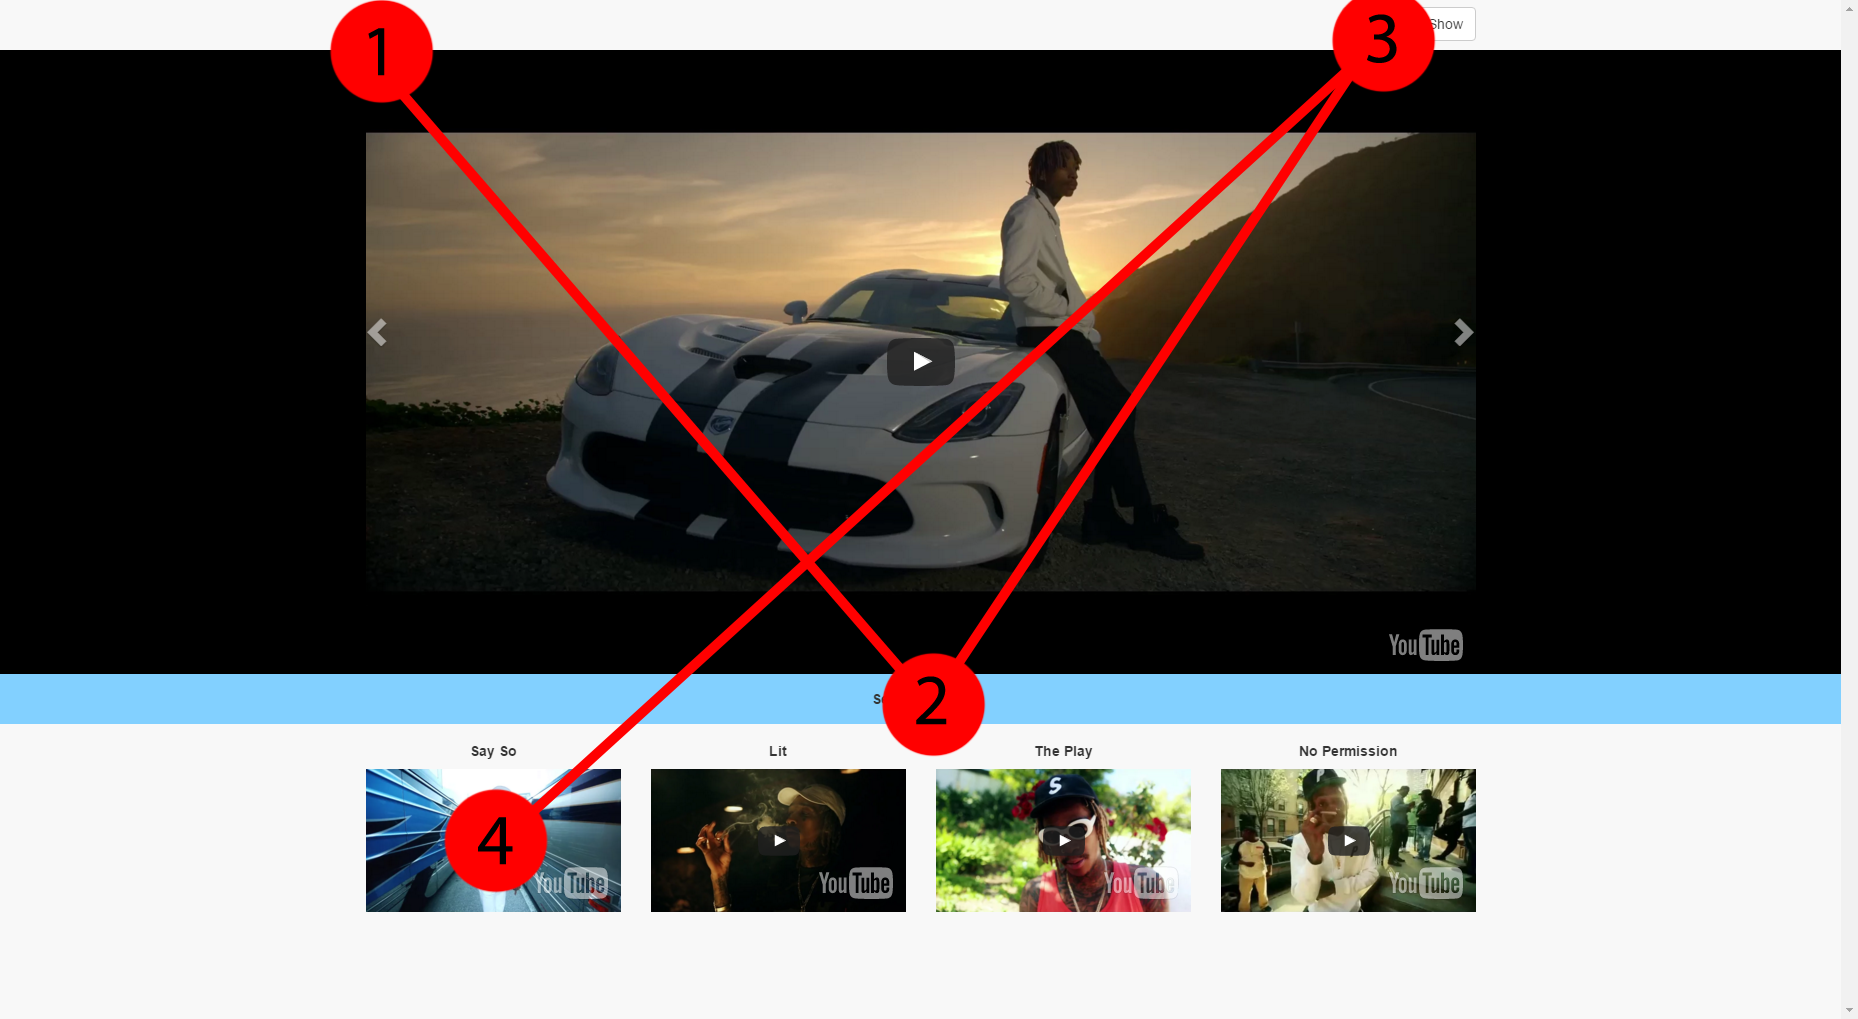
\includegraphics[width=0.48\textwidth]{p20}
  \end{center}
  \vspace{-20pt}
  \caption{Lecture du site}
  \vspace{-10pt}
\end{wrapfigure} 

Le bloc d'informations est la petite partie cach\'e du site qui regroupe toutes les informations sur un morceau de musique. J'ai volontairement cach\'e l'int\'erieur de cette partie car je souhaitais un site rapide \`a parcourir. L'oeil humain fonctionne par \'etape : progression, retour \`a la ligne et r\'egression. Mon but \'etait que l'utilisateur effectue en environs 1 seconde, la lecture enti\`ere d'une page du site. Il fallait donc que je limite le nombre de points de fixation (un point d'arr\^et dans la lecture). L'oeil s'arr\^etera entre 10 \`a 30 ms sur ces points. Mon site comporte 4 points d'arr\^ets comme on peux le voir sur la figure 13. Si j'avais laiss\'e mon bloc d'informations visible, il y aurait 7 points d'arr\^ets. \\

\begin{wrapfigure}{l}{0.5\textwidth}
  \vspace{-25pt}
  \begin{center}
    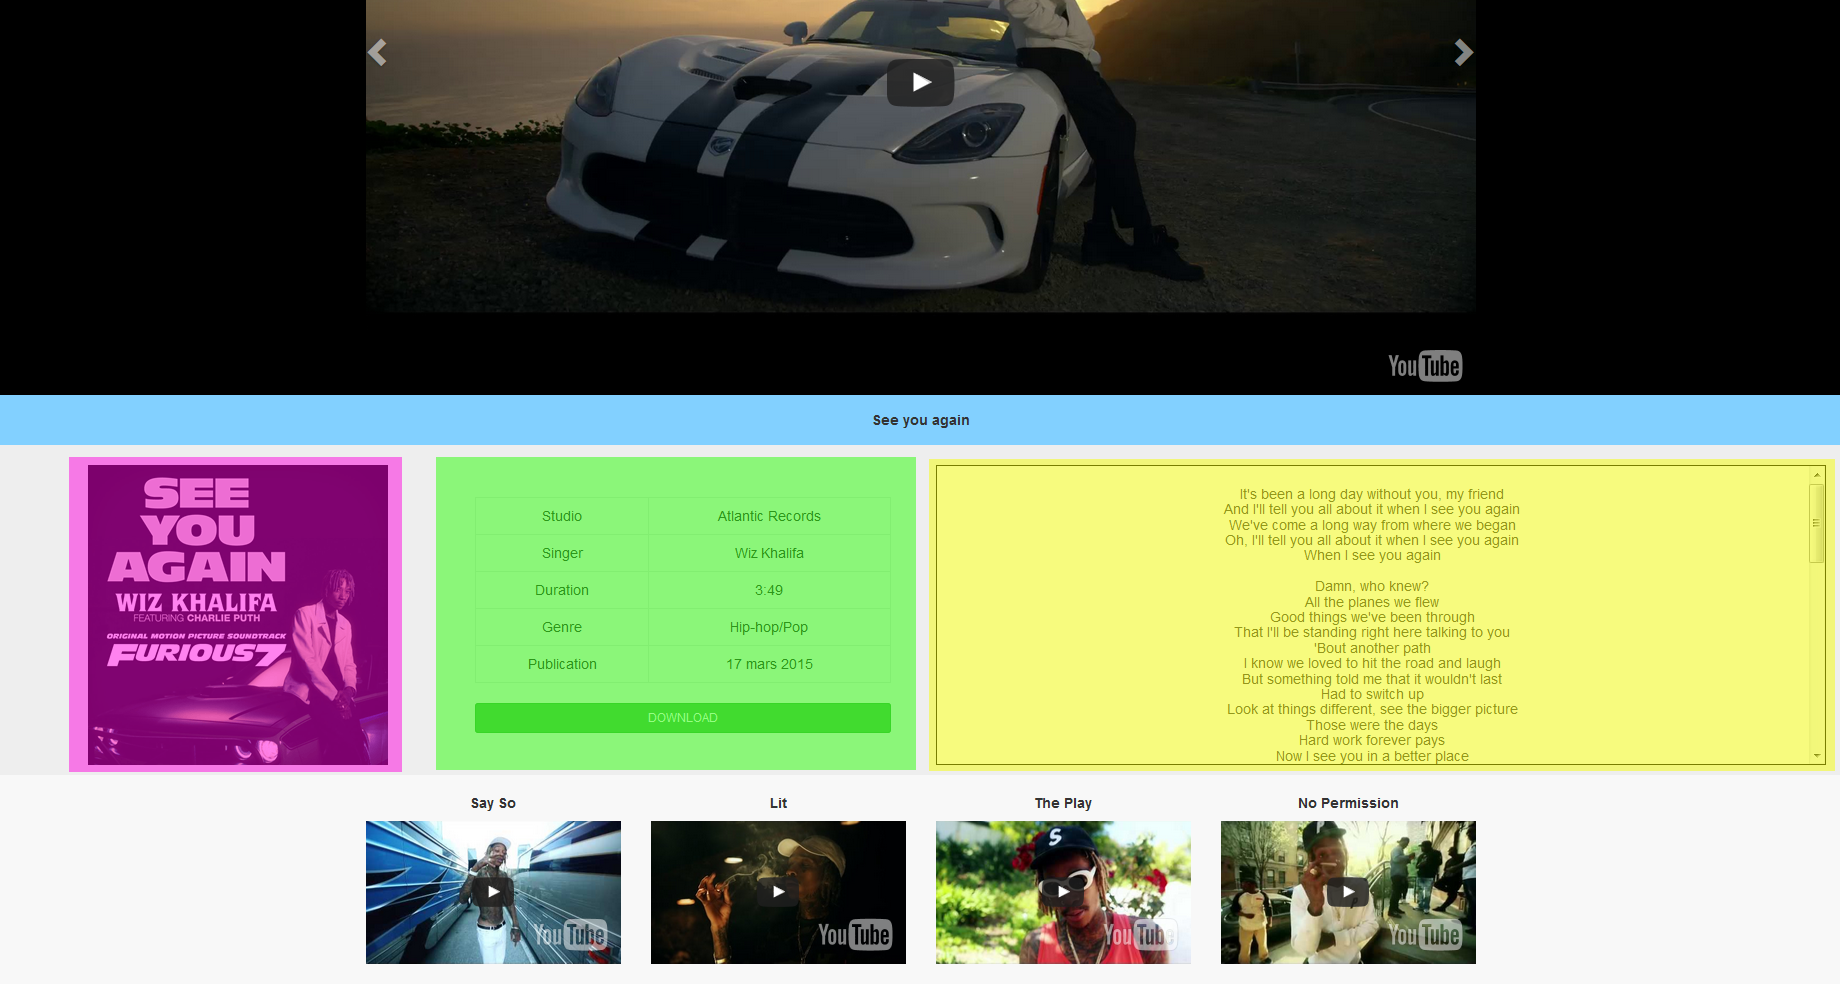
\includegraphics[width=0.48\textwidth]{p5}
  \end{center}
  \vspace{-20pt}
  \caption{Le bloc d'informations}
  \vspace{-10pt}
\end{wrapfigure} 

Les informations cach\'ees sont compos\'ees d'une image qui s'adapte \`a la largeur de la page, d'un tableau avec quelques informations sur le clips vid\'eos, d'un bouton pour t\'el\'echarger la musique au format MP3 et des paroles de la musique. L'ensemble de ces informations s'adapte \`a la largeur de la fen\^etre pour que la lecture ainsi que la manipulation soit la plus simple possible pour l'utilisateur. Notons que l'image disparait lorsque nous atteignons certains points de rupture (faible r\'esolutions). J'ai effectu\'e ce choix car je pense que l'utilisateur sur son t\'el\'ephone ne dispose pas forc\'ement d'une connexion ph\'enom\'enale comme on pourrait en avoir sur un ordinateur connect\'e en Ethernet. L'image n'\'etant pas une donn\'ee essentielle et prenant une part importante de ressources, j'ai jug\'e bon de la supprim\'e \`a basse r\'esolution pour le confort de l'utilisateur.\\

Sous Bootstrap, il n'y a rien de nouveau sur ce que j'ai cit\'e plus haut. Il s'agit maintenant seulement de placement des \'el\'ement dans une grille de positionnement. Le code ci-dessous r\'ealise ce que j'ai fait. Si il y a un point incompris, vous avez donc rat\'e un point dans mes explications pr\'ec\'edentes :
\vspace{0.5cm}\\
\fbox{\parbox{\textwidth}{
<div class="title text-center">\\
\hspace*{0.6cm}<strong><?php echo \$movie[0]['TITLE']; ?></strong>\\
</div>
}}
\vspace{0.5cm}\\
Ce petit bout de code permet d'afficher la barre de bleu avec le titre de la musique en son centre.Notons le petit emploie de PHP pour ne pas faire de travail trop r\'ep\'etitive entre mes pages.
\vspace{0.5cm}\\
\fbox{\parbox{\textwidth}{
<div class="hidden-xs hidden-sm col-md-6 col-lg-6 text-center pagination-centered">\\
\hspace*{0.6cm}<img src="<?php echo \$movie[0]['IMG']; ?>" class="img-responsive" alt="Responsive image">\\
</div>
}}
\vspace{0.5cm}\\
Ce code est celui qui servira pour afficher l'image. Comme on peux le voir l'image est "responsive" et sera cach\'ee lorsque la largeur de la fen\^etre sera inf\'erieur \`a \og sm \fg{}.
\vspace{0.5cm}\\
\fbox{\parbox{\textwidth}{
<div class="col-md-6 col-lg-6 text-center pagination-centered center-block" style="display: flex;">\\
\hspace*{0.6cm}<div style="align-self: center;width:100\%;">\\
\hspace*{0.6cm}<table class="table table-bordered">\\
\hspace*{1.2cm}<tbody>\\
\hspace*{1.8cm}<tr>\\
\hspace*{2.4cm}<td>Studio</td>\\
\hspace*{2.4cm}<td><?php echo \$movie[0]['STUDIO']; ?></td>\\
\hspace*{1.8cm}</tr>\\
\hspace*{1.8cm}<tr>\\
\hspace*{2.4cm}<td>Singer</td>\\
\hspace*{2.4cm}<td><?php echo \$movie[0]['SINGER']; ?></td>\\
\hspace*{1.8cm}</tr>\\
\hspace*{1.8cm}<tr>\\
\hspace*{2.4cm}<td>Duration</td>\\
\hspace*{2.4cm}<td><?php echo \$movie[0]['DURATION']; ?></td>\\
\hspace*{1.8cm}</tr>\\
\hspace*{1.8cm}<tr>\\
\hspace*{2.4cm}<td>Genre</td>\\
\hspace*{2.4cm}<td><?php echo \$movie[0]['GENRE']; ?></td>\\
\hspace*{1.8cm}</tr>\\
\hspace*{1.8cm}<tr>\\
\hspace*{2.4cm}<td>Publication</td>\\
\hspace*{2.4cm}<td><?php echo \$movie[0]['PUBLICATION']; ?></td>\\
\hspace*{1.8cm}</tr>\\
\hspace*{1.2cm}</tbody>\\
\hspace*{0.6cm}</table>\\
\hspace*{0.6cm}<a href="ddl/<?php echo \$movie[0]['CODE']; ?>.mp3" class="btn btn-success btn-sm full" download>DOWNLOAD</a>\\
\hspace*{0.6cm}</div>\\
</div>
}}
\vspace{0.5cm}\\
Le tableau est \'evidement lui aussi compos\'e d'un peu de PHP. Il n'y a rien d'exceptionnel, il s'agit seulement d'une balise TABLE utilisant le style de Boostrap avec la classe \og table \fg{}. A noter ici, la petite astuce qui permet au tableau de prendre 100\% de l'espace lorsque l'image disparait. Je n'ai pas sp\'ecifi\'e volontairement le fait que le tableau prenne 12 colonnes, je n'ai rien mis pour les petites r\'esolutions car par d\'efaut Bootstrap force les \'el\'ements \`a prendre le plus d'espace possible. Je n'ai donc pas eu \`a le rajouter. 
\vspace{0.5cm}\\
\fbox{\parbox{\textwidth}{
<div class="col-md-12 col-lg-6">\\
\hspace*{0.6cm}<div class="text-center write">\\
\hspace*{1.2cm}<h2><?php echo \$movie[0]['LYRIC']; ?></h2>\\
\hspace*{0.6cm}</div>\\
</div>
}}
\vspace{0.5cm}\\
Ce bloc fait r\'ef\'erence au parole de la chanson. J'ai utilis\'e la balise H2 pour faire du \og responsive typesetting \fg{}. La taille en pixel du texte varie suivant la taille de la fen\^etre. Pour l'utilisateur, il est sans aucun doute plus agr\'eable de pouvoir lire les paroles d'une chanson phrase par phrase. Or, si la taille du texte restait la m\^eme pour toutes dimensions de fen\`etre, soit le texte serait illisible \`a une grande r\'esolution, soit le site serait incommode \`a basse r\'esolution. Pour r\'esoudre ce probl\`eme, une proportion a \'et\'e sp\'ecifi\'e pour l'ensemble des textes suivant la largeur de la fen\`etre ou de l'appareil. Sur le site, on retrouve cette particularit\'e sur plusieurs titres et sur les paroles comme nous pouvons le constater ci-dessous. \`A gauche, on retrouve les paroles des chansons sur t\'el\'ephone portable tandis que \`a droite, on retrouve les m\^emes paroles \'ecrite avec une plus grande police sur tablette.

\begin{center}
\vspace{0.5cm}
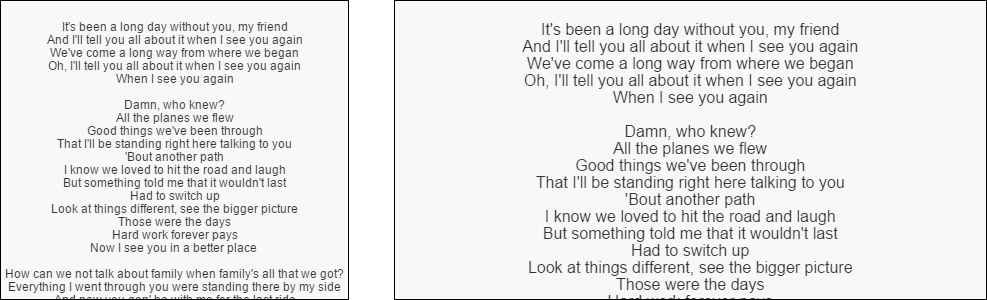
\includegraphics[width=0.8\textwidth]{textes}
\vspace{0.5cm}\\
\end{center}
Avec l'ensemble de ces parties de code, on arrive \`a reproduire notre bloc d'informations sous Bootstrap, il s'agissait bien comme je le disais en d\'ebut de partie d'une affaire de positionnement.\\
Sous Polymer, le code est moins long et moins complexe \`a mes yeux. Cependant, il faut l\`a encore cr\'eer un gros nombre de nouveaux modules, ce qui repr\'esente un travail fastidieux et long. Le code dans l'index se r\'esume \`a cela :
\vspace{0.5cm}\\
\fbox{\parbox{\textwidth}{
<bloc-information>\\
\hspace*{0.6cm}<my-col-50-100>\\
\hspace*{1.2cm}<my-col-50-50>\\
\hspace*{1.8cm}<my-col-hidden-1200>\\
\hspace*{1.8cm}<my-img-responsive link="<?php echo \$movie[0]['IMG']; ?>"></my-img-responsive>\\
\hspace*{1.8cm}</my-col-hidden-1200>\\
\hspace*{1.2cm}</my-col-50-50>\\
\hspace*{1.2cm}<my-col-50-50>\\
\hspace*{1.8cm}<my-informations studio="<?php echo \$movie[0]['STUDIO']; ?>" singer="<?php echo \$movie[0]['SINGER']; ?>" duration="<?php echo \$movie[0]['DURATION']; ?>" genre="<?php echo \$movie[0]['GENRE']; ?>" publication="<?php echo \$movie[0]['PUBLICATION']; ?>" download="ddl/<?php echo \$movie[0]['CODE']; ?>.mp3"></my-informations>\\
\hspace*{1.2cm}</my-col-50-50>\\
\hspace*{0.6cm}</my-col-50-100>\\
\hspace*{0.6cm}<my-col-50-100>\\
\hspace*{1.2cm}<my-lyric>\\
\hspace*{1.8cm}<?php echo \$movie[0]['LYRIC']; ?>\\
\hspace*{1.2cm}</my-lyric>\\
\hspace*{0.6cm}</my-col-50-100>\\
</bloc-information>
}}
\vspace{0.5cm}\\
Je vais \'evidemment expliquer l'ensemble de mes modules ci-dessous. Je tiens avant d'indiquer que l'utilisation de PHP est proscrite dans les modules que l'on cr\'e\'e, il faut donc faire en sorte que le module puisse avoir des attributs. Ce qui explique pourquoi ma balise MY-INFORMATION prend beaucoup d'informations.\\
\vspace{0.5cm}\\
\fbox{\parbox{\textwidth}{
<dom-module id="my-informations">\\
\hspace*{0.6cm}<template>\\
\hspace*{0.6cm}<style>	\\
\hspace*{0.6cm}...(se reporter \`a mon GIT ou voir sur Bootstrap pour avoir le style exact)\\
\hspace*{0.6cm}</style>	\\
\hspace*{0.6cm}<div style="display: flex;">\\
\hspace*{0.6cm}<div style="align-self: center;width:100\%;">	\\
\hspace*{0.6cm}<table class="table table-bordered">\\
\hspace*{0.6cm}<tbody>\\
\hspace*{0.6cm}<tr>\\
\hspace*{0.6cm}<td>Studio</td>\\
\hspace*{0.6cm}<td>\{\{studio\}\}</td>\\
\hspace*{0.6cm}</tr>\\
\hspace*{0.6cm}<tr>\\
\hspace*{0.6cm}<td>Singer</td>\\
\hspace*{0.6cm}<td>\{\{singer\}\}</td>\\
\hspace*{0.6cm}</tr>\\
\hspace*{0.6cm}<tr>\\
\hspace*{0.6cm}<td>Duration</td>\\
\hspace*{0.6cm}<td>\{\{duration\}\}</td>\\
\hspace*{0.6cm}</tr>\\
\hspace*{0.6cm}<tr>\\
\hspace*{0.6cm}<td>Genre</td>\\
\hspace*{0.6cm}<td>\{\{genre\}\}</td>\\
\hspace*{0.6cm}</tr>\\
\hspace*{0.6cm}<tr>\\
\hspace*{0.6cm}<td>Publication</td>\\
\hspace*{0.6cm}<td>\{\{publication\}\}</td>\\
\hspace*{0.6cm}</tr>\\
\hspace*{0.6cm}</tbody>\\
\hspace*{0.6cm}</table>	\\
\hspace*{0.6cm}<a href="\{\{download\}\}" class="btn btn-success btn-sm full" download>DOWNLOAD</a>\\
\hspace*{0.6cm}</div>	\\
\hspace*{0.6cm}</div>\\		
\hspace*{0.6cm}</template>\\
\hspace*{0.6cm}<script>\\
\hspace*{0.6cm}\color{red}{Polymer(\{\\
\hspace*{0.6cm}is: "my-informations",\\
\hspace*{0.6cm}properties: \{\\
\hspace*{0.6cm}link: String,\\
\hspace*{0.6cm}studio: String,\\
\hspace*{0.6cm}singer: String,\\
\hspace*{0.6cm}duration: String,\\
\hspace*{0.6cm}genre: String,\\
\hspace*{0.6cm}publication: String,\\
\hspace*{0.6cm}download: String\\
\hspace*{0.6cm}\}\\
\hspace*{0.6cm}\});}\\
\hspace*{0.6cm}\color{black}{</script> \\
</dom-module>}
}}
\vspace{0.5cm}\\
Ce module repr\'esente le tableau avec toutes ces informations. Ici, j'ai utilis\'e comme dit plus haut des propri\'et\'es pour cet \'el\'ement. En rouge, on trouve les propri\'et\'es du bloc, j'ai d\'efini ces derni\`eres comme des strings. Pour ensuite, les utiliser dans le bloc, il suffit d'\'ecrire \{\{ NOM DE LA PROPRIETE \}\}.
\vspace{0.5cm}\\
\fbox{\parbox{0.5\textwidth}{
<dom-module id="my-col-50-50">\\
\hspace*{0.6cm}<template>\\
\hspace*{1.2cm}<style>		\\
\hspace*{1.2cm}:host \{		\\
\hspace*{1.8cm}position: relative;\\
\hspace*{1.8cm}min-height: 1px;\\
\hspace*{1.8cm}padding-left: 15px;\\
\hspace*{1.8cm}padding-right: 15px;\\
\hspace*{1.8cm}float:left;\\
\hspace*{1.8cm}width:50\%;\\
\hspace*{1.8cm}box-sizing: border-box;\\
\hspace*{1.8cm}vertical-align:middle;\\
\hspace*{1.2cm}\}\\
\hspace*{1.2cm}@media (max-width:1500px) \{\\
\hspace*{1.8cm}:host \{\\
\hspace*{2.4cm}margin-bottom: 20px;\\
\hspace*{1.8cm}\}\\
\hspace*{1.2cm}\}	\\
\hspace*{1.2cm}@media (max-width:1200px) \{\\
\hspace*{1.8cm}:host \{\\
\hspace*{2.4cm}width:100\%;\\
\hspace*{2.4cm}margin-bottom: 0px;\\
\hspace*{1.8cm}\}\\
\hspace*{1.2cm}\}\\
\hspace*{1.2cm}</style>	\\
\hspace*{1.2cm}<content></content>\\
\hspace*{0.6cm}</template>\\
\hspace*{0.6cm}<script>\\
\hspace*{1.2cm}Polymer(\{\\
\hspace*{1.8cm}is: "my-col-50-50"\\
\hspace*{1.2cm}\});\\
\hspace*{0.6cm}</script>\\
</dom-module>
}}
\fbox{\parbox{0.5\textwidth}{
<dom-module id="my-col-50-100">\\
\hspace*{0.6cm}<template>\\
\hspace*{1.2cm}<style>	\\
\hspace*{1.8cm}:host \{	\\	
\hspace*{2.4cm}position: relative;\\
\hspace*{2.4cm}min-height: 1px;\\
\hspace*{2.4cm}padding-left: 15px;\\
\hspace*{2.4cm}padding-right: 15px;\\
\hspace*{2.4cm}float:left;\\
\hspace*{2.4cm}width:50\%;\\
\hspace*{2.4cm}box-sizing: border-box;\\
\hspace*{1.8cm}\}\\
\hspace*{1.8cm}@media (max-width:1500px) \{\\
\hspace*{2.4cm}:host \{\\
\hspace*{3.0cm}width:100\%;\\
\hspace*{2.4cm}\}\\
\hspace*{1.8cm}\}\\
\hspace*{1.8cm}</style>\\
\hspace*{1.8cm}<content></content>\\
\hspace*{1.2cm}</template>\\
\hspace*{1.2cm}<script>\\
\hspace*{1.2cm}Polymer(\{\\
\hspace*{1.8cm}is: "my-col-50-100"\\
\hspace*{1.2cm}\});\\
\hspace*{0.6cm}</script>\\
</dom-module>
}}
\vspace{0.5cm}\\
Comme vu pr\'ec\'edemment, ce sont ces modules qui joueront le r\^ole de positionnement sous Polymer. L'utilisation des m\'edia queries permet de fixer la taille de la zone dont dispose l'\'el\'ement en fonction de la largeur de l'\'ecran.
\vspace{0.5cm}\\
\fbox{\parbox{\textwidth}{
<dom-module id="my-img-responsive">\\
\hspace*{0.6cm}<template>\\
\hspace*{1.2cm}<style>		\\
\hspace*{1.8cm}:host \{	\\	
\hspace*{2.4cm}width:100\%;\\
\hspace*{2.4cm}height: auto;\\
\hspace*{1.8cm}\}		\\
\hspace*{1.2cm}</style>\\
\hspace*{1.2cm}<img src="{{link}}"></img>\\
\hspace*{0.6cm}</template>\\
\hspace*{0.6cm}<script>\\
\hspace*{1.2cm}Polymer(\{\\
\hspace*{1.8cm}is: "my-img-responsive",\\
\hspace*{1.8cm}properties: { link: String }\\
\hspace*{1.2cm}\});\\
\hspace*{0.6cm}</script>\\
</dom-module>
}}
\vspace{0.5cm}\\
Ce module permet de faire des images responsives. Comme dit au tout d\'epart de mon document. Une image responsive n'est qu'une image avec un largeur de 100\% et une hauteur fonction de son ratio. Dans ce module, j'ai aussi ajout\'e une propri\'et\'e qui est bien \'evidemment l'adresse de l'image en question.
\vspace{0.5cm}\\
\fbox{\parbox{\textwidth}{
<dom-module id="my-lyric">\\
\hspace*{0.6cm}<template>\\
\hspace*{1.2cm}<style>	\\
\hspace*{1.8cm}:host \{	\\	
\hspace*{2.4cm}display: block;\\
\hspace*{2.4cm}overflow-y: scroll;\\
\hspace*{2.4cm}max-height: 300px;\\
\hspace*{2.4cm}background: \#F8F8F8 none repeat scroll 0\% 0\%;\\
\hspace*{2.4cm}border: 1px solid \#000;\\
\hspace*{2.4cm}text-align: center;\\
\hspace*{2.4cm}box-sizing: border-box;\\
\hspace*{2.4cm}padding-top: 20px;\\
\hspace*{1.8cm}\}	\\	
\hspace*{1.8cm}h2 \{\\
\hspace*{2.4cm}font-family: inherit;\\
\hspace*{2.4cm}font-weight: 500;\\
\hspace*{2.4cm}line-height: 1.1;\\
\hspace*{2.4cm}color: inherit;\\
\hspace*{2.4cm}font-size: 14px;\\
\hspace*{1.8cm}\}	\\
\hspace*{1.8cm}@media(max-width:600px)\{\\
\hspace*{2.4cm}h2\{font-size: 10px;\}\\
\hspace*{1.8cm}\}	\\
\hspace*{1.8cm}@media(min-width:601px)\{\\
\hspace*{2.4cm}h2\{font-size: 14px;\}\\
\hspace*{1.8cm}\}\\	
\hspace*{1.8cm}@media(min-width:1200px)\{\\
\hspace*{2.4cm}h2\{font-size: 14px;\}\\
\hspace*{1.8cm}\}		\\
\hspace*{1.8cm}@media(min-width:1500px)\{\\
\hspace*{2.4cm}h2\{font-size: 14px;\}\\
\hspace*{1.8cm}\}	\\
\hspace*{1.2cm}</style>\\
\hspace*{1.2cm}<div><h2><content></content></h2></div>\\
\hspace*{0.6cm}</template>\\
\hspace*{0.6cm}<script>\\
\hspace*{1.2cm}Polymer(\{\\
\hspace*{1.8cm}is: "my-lyric", \\
\hspace*{1.8cm}properties: \{\\
\hspace*{2.4cm}link: String\\
\hspace*{1.8cm}\}\\
\hspace*{1.2cm}\});\\
\hspace*{0.6cm}</script> \\
</dom-module>
}}
\vspace{0.5cm}\\
Le module \og my-lyric \fg{} repr\'esente le petit bloc avec les paroles de la chanson. Comme dit pr\'ec\'emment, je r\'ealise ici un changement de police suivant la largeur de la fen\^etre. J'ai d\'ej\`a expliqu\'e pourquoi j'ai fait ce choix mais je n'avais pas encore montr\'e la mani\`ere de proc\'ec\'d\'e. Il s'agit comme on peux le voir d'un simple changement de la taille de la police.\\
\vspace{0.5cm}\\
\fbox{\parbox{\textwidth}{
<dom-module id="my-col-hidden-1200">\\
\hspace*{0.6cm}<template>\\
\hspace*{1.2cm}<style>			\\	
\hspace*{1.8cm}@media (max-width:1200px) \{\\
\hspace*{2.4cm}:host \{\\
\hspace*{3.0cm}display: none;\\
\hspace*{2.4cm}\}\\
\hspace*{1.8cm}\}\\
\hspace*{1.2cm}</style>\\	
\hspace*{1.2cm}<content></content>\\
\hspace*{1.2cm}</template>\\
\hspace*{0.6cm}<script>\\
\hspace*{0.6cm}Polymer(\{\\
\hspace*{1.2cm}is: "my-col-hidden-1200"\\
\hspace*{0.6cm}\});\\
\hspace*{0.6cm}</script>\\
</dom-module>
}}
\vspace{0.5cm}\\
Ce dernier module est ici pour reproduire le comportement de la classe \og col-hidden-sm \fg{}. C'est \`a dire que ce module permet de supprimer un \'el\'ement \`a partir d'une certaine largeur de fen\`etre (1200px dans ce cas).\\
Avec toutes ces informations, nous sommes maintenant capable de reproduire ce que j'ai r\'ealis\'e. Il ne reste plus qu'\`a reproduire le comportement pour cacher ou afficher ces informations. Ce m\'echanisme est produit via JQuery avec les m\'ethodes \og slide-toggle \fg{} et \og clic \fg{} :  
\vspace{0.5cm}\\
\fbox{\parbox{\textwidth}{
\$( "my-bar-title" ).click(function() \{\\
\hspace*{0.6cm}\$( "bloc-information" ).slideToggle( "fast");\\
\});
}}
\vspace{0.5cm}\\

\subsection{Clips vid\'eos suppl\'ementaires}

Les clips vid\'eos suppl\'ementaires sont les vid\'eos qui se trouvent en bas de la page. Ces vid\'eos sont au nombre de 4 \`a grandes r\'esolutions et au nombres de 2 \`a basses r\'esolutions. Pour bien comprendre pourquoi j'ai fait ce choix, colorions chaque divisions de cette partie du site d'une couleur unique.
\begin{center}
\vspace{0.5cm}
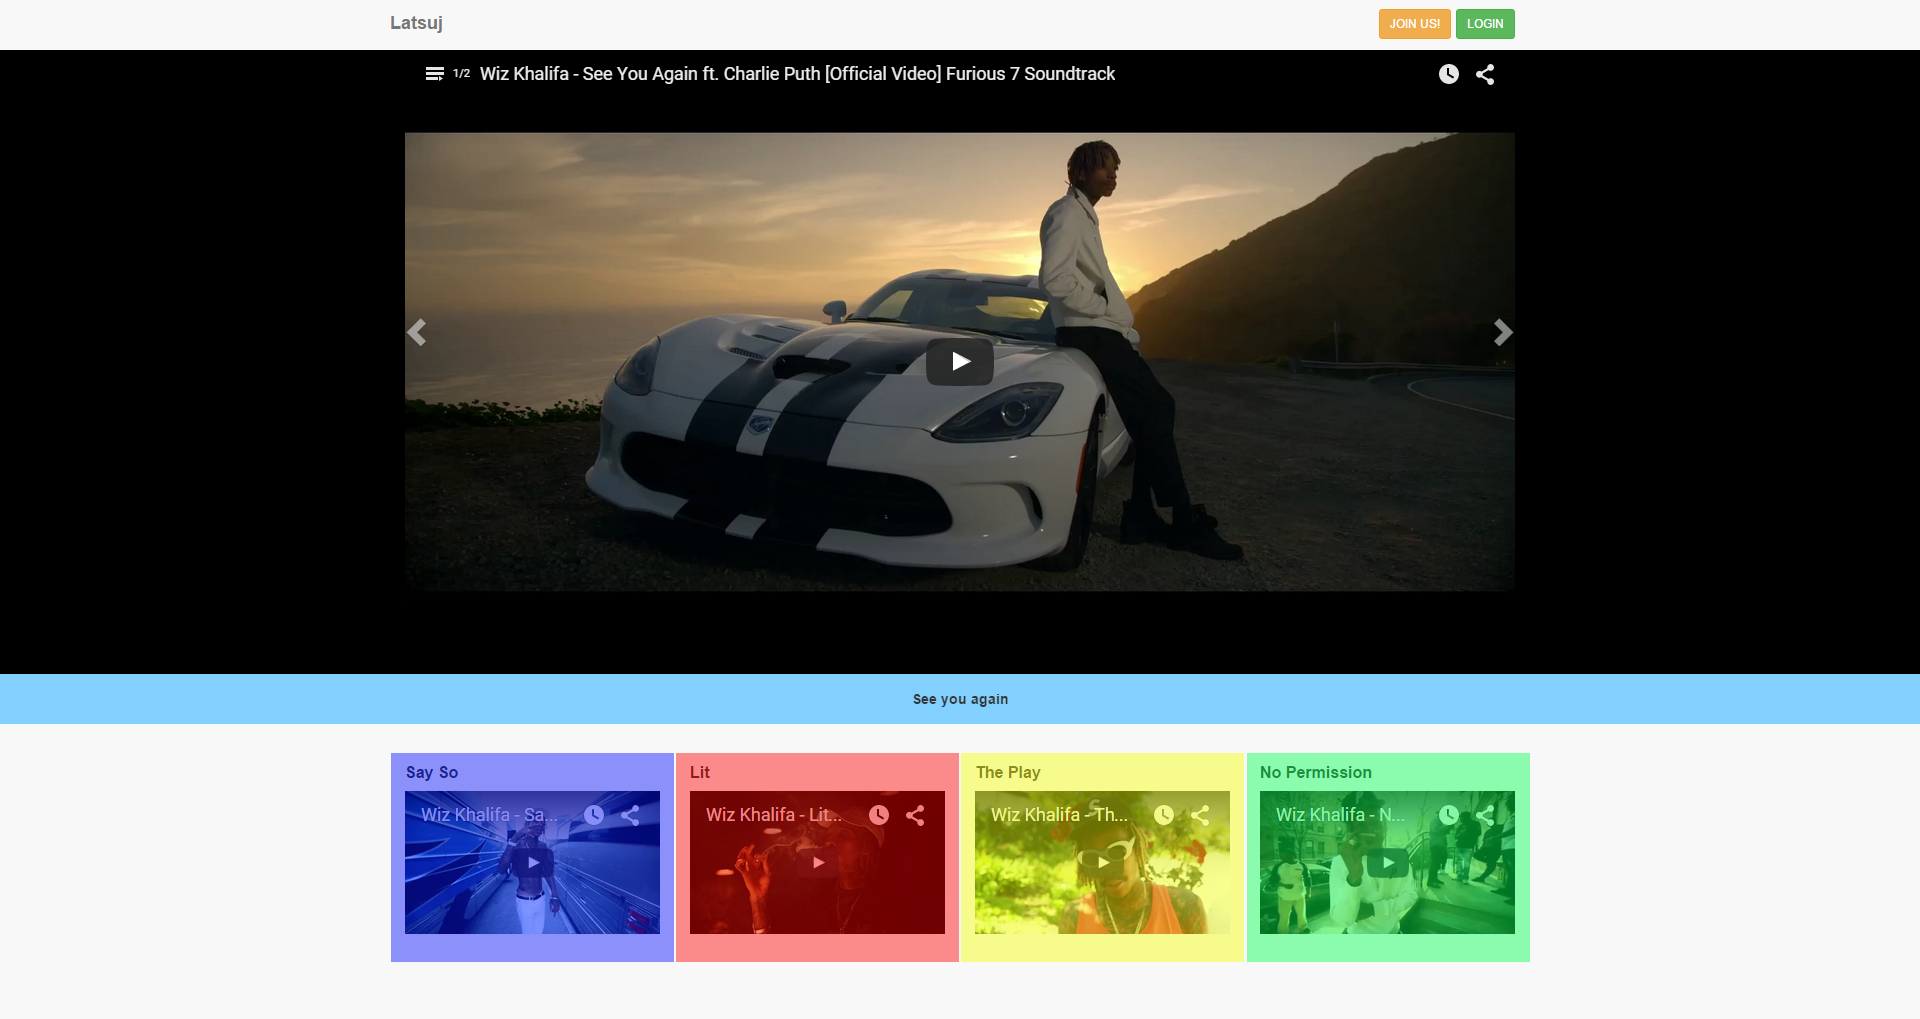
\includegraphics[width=0.8\textwidth]{pc4}
\vspace{0.5cm}
\end{center}

Si nous r\'eduisons la largeur de la fen\^etre, le contenu s'adaptera. Dans un premier temps, il n'y aura plus que deux blocs par ligne. Puis, si nous continuons de r\'eduire la fen\^etre, il n'y aura plus qu'un seul bloc par ligne et les deux derniers auront \'et\'e cach\'e.
\begin{center}
\vspace{0.5cm}
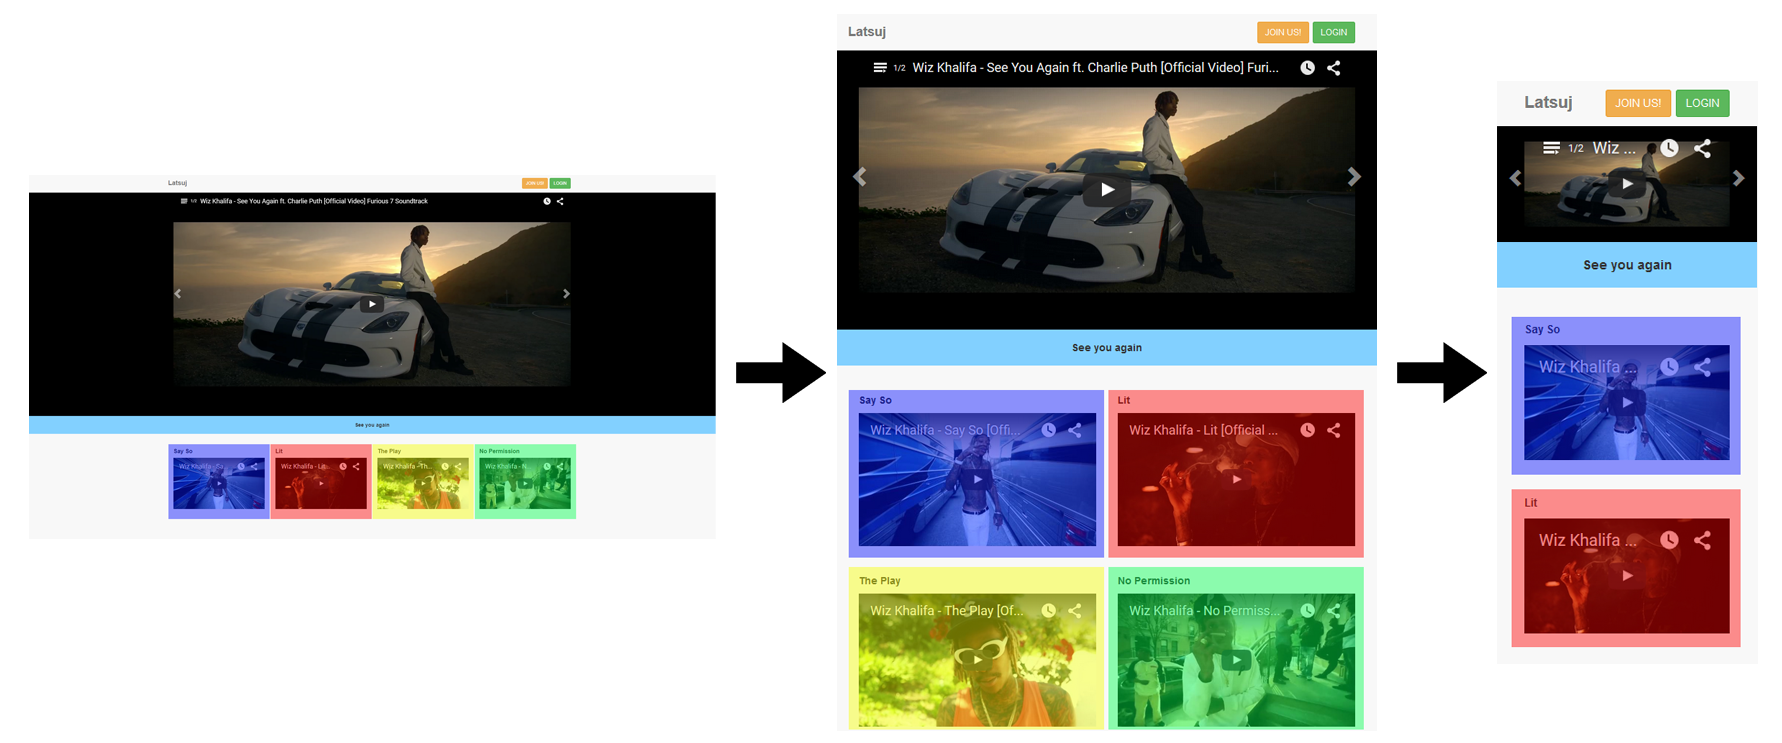
\includegraphics[width=0.8\textwidth]{pc7}
\vspace{0.5cm}\\
\end{center}

\hspace*{0.6cm}Pourquoi ai-je supprim\'e les deux derniers blocs sur la navigation \`a basse r\'esolution ? Ce n'est pas une d\'ecision anodine. En supprimant ces deux blocs, j'am\'eliore l'exp\'erience de l'utilisateur sur deux aspects.\\
\begin{wrapfigure}{r}{3cm}
\vspace{-13pt}
\centering
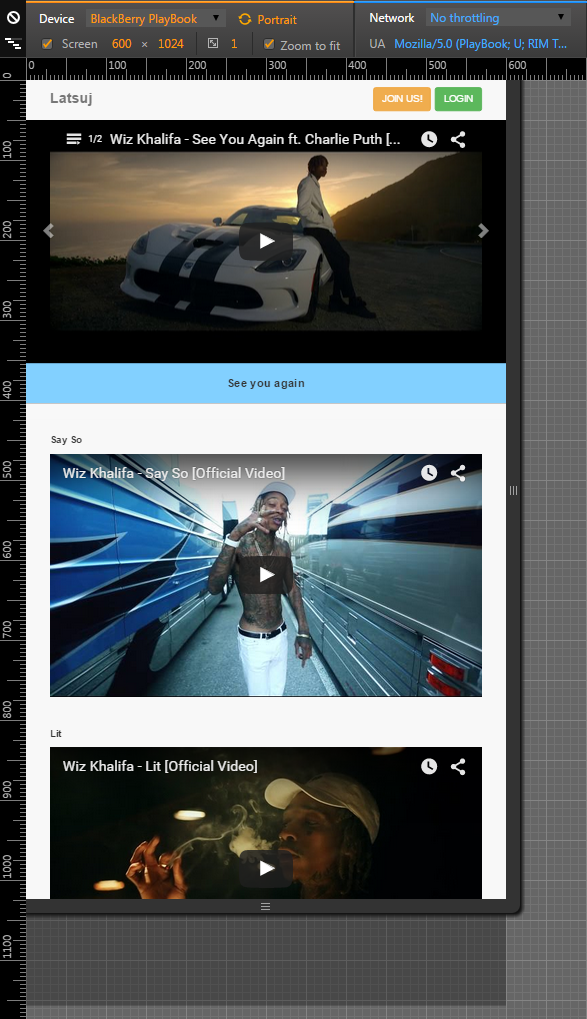
\includegraphics[width=3cm]{blackberry}
\caption{\textit{Affichage du site sous BlackBerry (via Google Chrome).}}
\end{wrapfigure} 
{\hspace*{0.6cm}L'un est purement li\'e \`a la technologie, il est rare d'avoir un t\'el\'ephone branch\'e en Ethernet. Ceci implique que le d\'ebit moyen d'un utilisateur sur t\'el\'ephone est souvent inf\'erieur \`a celui d'un utilisateur sur ordinateur. J'\'evite ainsi \`a l'utilisateur sur t\'el\'ephone de charger trop d'informations qui n'appartiennent pas au contenu principal de la page. Ce ne sont que des publicit\'es pour les autres musiques du m\^eme chanteur. Deuxi\`emement, et c'est sans doute le point le plus important, suivant \textbf{la loi de Fitt}, que je sois sur t\'el\'ephone ou ordinateur l'indice de difficult\'e doit rester le m\^eme. La loi calcul un indice de difficult\'e par rapport au temps requis pour aller rapidement d'une position de d\'epart \`a une zone finale de destination. L'utilisateur doit arriver avec la m\^eme rapidit\'e et la m\^eme facilit\'e aux diff\'erentes parties du site. Si l'on regarde l'image sur la droite qui repr\'esente le site sur un t\'el\'ephone BlackBerry, on remarque que le temps pour parvenir \`a la derni\`ere vid\'eo en rapport avec le chanteur est aussi rapide sur le t\'el\'ephone que sur ordinateur. Certes ce n'est pas la m\^eme, mais cela reste la derni\`ere vid\'eo. Si j'avais juste r\'earrang\'e les choses, il aurait d'abord fallu descendre pour arriver \`a la derni\`ere vid\'eo. Cela ne para\^it pas beaucoup plus compliqu\'e mais sans cela, le site se retrouverait complexifi\'e d'apr\`es la loi de Fitts.}\\

Que cela soit sur Bootstrap ou Polymer, nous savons normalement comment faire cela \`a partir des informations et techniques que nous avons d\'ej\`a \'evoqu\'e jusqu'ici. Cette partie reprend le positionnement et l'affichage ou le non affichage de certaines informations en fonction de la largeur de la fen\^etre.
\vspace{0.5cm}\\
\fbox{\parbox{\textwidth}{
<nav class="navbar navbar-default navbar-static-bottom">\\
\hspace*{1.2cm}<div class="container">\\
\hspace*{1.8cm}<div class="row">\\
\hspace*{2.4cm}<div class="col-xs-push col-sm-6 col-md-6 col-lg-3 text-center">\\
\hspace*{3.0cm}<h2><strong><?php echo \$pubs[0]['TITLE1']; ?></strong></h2>\\
\hspace*{3.0cm}<div class="embed-responsive embed-responsive-16by9">\\
\hspace*{3.0cm}<iframe class="embed-responsive-item" src="https://www.youtube.com/embed/ <?php echo \$pubs[0]['LINK1']; ?>?showinfo=0\&controls=0"></iframe>\\
\hspace*{3.0cm}</div>\\
\hspace*{2.4cm}</div>\\
\hspace*{2.4cm}<div class="col-xs-push col-sm-6 col-md-6 col-lg-3 text-center">\\
\hspace*{3.0cm}<h2><strong><?php echo \$pubs[0]['TITLE2']; ?></strong></h2>\\
\hspace*{3.0cm}<div class="embed-responsive embed-responsive-16by9">\\
\hspace*{3.0cm}<iframe class="embed-responsive-item" src="https://www.youtube.com/embed/ <?php echo \$pubs[0]['LINK2']; ?>?showinfo=0\&controls=0"></iframe>\\
\hspace*{3.0cm}</div>\\
\hspace*{2.4cm}</div>\\
\hspace*{2.4cm}<div class="hidden-xs col-sm-6 col-md-6 col-lg-3 text-center">\\
\hspace*{3.0cm}<h2><strong><?php echo \$pubs[0]['TITLE3']; ?></strong></h2>\\
\hspace*{3.0cm}<div class="embed-responsive embed-responsive-16by9">\\
\hspace*{3.0cm}<iframe class="embed-responsive-item" src="https://www.youtube.com/embed/ <?php echo \$pubs[0]['LINK3']; ?>?showinfo=0\&controls=0"></iframe>\\
\hspace*{3.0cm}</div>\\
\hspace*{2.4cm}</div>\\
\hspace*{2.4cm}<div class="hidden-xs col-sm-6 col-md-6 col-lg-3 text-center">\\
\hspace*{3.0cm}<h2><strong><?php echo \$pubs[0]['TITLE4']; ?></strong></h2>\\
\hspace*{3.0cm}<div class="embed-responsive embed-responsive-16by9">\\
\hspace*{3.0cm}<iframe class="embed-responsive-item" src="https://www.youtube.com/embed/ <?php echo \$pubs[0]['LINK4']; ?>?showinfo=0\&controls=0"></iframe>\\
\hspace*{3.0cm}</div>\\
\hspace*{2.4cm}</div>\\
\hspace*{1.8cm}</div>\\
\hspace*{1.2cm}</div>\\
</nav>
}}
\vspace{0.5cm}\\
Sous Bootstrap, il faut donc simplement d\'efinir le nombre de colonne utilis\'e par chaque petit bloc. La moiti\'e seront d\'efini comme \og hidden \fg{} comme on peux l'observer sur le code. Sous Polymer, cela sera beaucoup plus rapide car cela reprend une grosse partie des modules qui ont \'et\'e d\'efini pr\'ec\'edemment, ainsi le code devient plus facile \`a impl\'ementer car il n'y a presque pas de nouveaux modules :
\vspace{0.5cm}\\
\fbox{\parbox{\textwidth}{
<my-bar-pubs>\\
\hspace*{0.6cm}<my-container>\\
\hspace*{1.2cm}<my-col-25-100>\\
\hspace*{2.4cm}<resp-div name="<?php echo \$pubs[0]['TITLE1']; ?>" link="https:// www.youtube.com/embed/<?php echo \$pubs[0]['LINK1']; ?>?showinfo=0\&controls=0"></resp-div>\\
\hspace*{1.2cm}</my-col-25-100>\\
\hspace*{1.2cm}<my-col-25-100>\\
\hspace*{2.4cm}<resp-div name="<?php echo \$pubs[0]['TITLE2']; ?>" link="https:// www.youtube.com/embed/<?php echo \$pubs[0]['LINK2']; ?>?showinfo=0\&controls=0"></resp-div>\\
\hspace*{1.2cm}</my-col-25-100>\\
\hspace*{1.2cm}<my-col-hidden-900>\\
\hspace*{1.8cm}<my-col-25-100>\\
\hspace*{2.4cm}<resp-div name="<?php echo \$pubs[0]['TITLE3']; ?>" link="https:// www.youtube.com/embed/<?php echo \$pubs[0]['LINK3']; ?>?showinfo=0\&controls=0"></resp-div>\\
\hspace*{1.8cm}</my-col-25-100>\\
\hspace*{1.2cm}</my-col-hidden-900>\\
\hspace*{1.2cm}<my-col-hidden-900>\\
\hspace*{1.8cm}<my-col-25-100>\\
\hspace*{2.4cm}<resp-div name="<?php echo \$pubs[0]['TITLE4']; ?>" link="https:// www.youtube.com/embed/<?php echo \$pubs[0]['LINK4']; ?>?showinfo=0\&controls=0"></resp-div>\\
\hspace*{1.8cm}</my-col-25-100>\\
\hspace*{1.2cm}</my-col-hidden-900>\\
\hspace*{0.6cm}</my-container>\\
</my-bar-pubs>
}}
\vspace{0.5cm}\\
Ce code reproduit donc le comportement pr\'ec\'edent sur Polymer. Il n'y a rien normalement qui ne vous soit inconnu ici \`a part le \og my-bar-pubs \fg{} mais il s'agit simplement d'une barre avec une couleur en fond comme on peux le voir ci-dessous : 
\vspace{0.5cm}\\
\fbox{\parbox{\textwidth}{
<dom-module id="my-bar-pubs">\\
\hspace*{0.6cm}<template>\\
\hspace*{1.2cm}<style>\\		
\hspace*{1.8cm}:host \{	\\	
\hspace*{2.4cm}background-color: \#f8f8f8;\\
\hspace*{2.4cm}text-align: center;\\
\hspace*{2.4cm}float: left;\\
\hspace*{2.4cm}width: 100\%;\\
\hspace*{2.4cm}box-sizing: border-box;\\
\hspace*{1.8cm}\}\\
\hspace*{1.2cm}</style>\\
\hspace*{1.2cm}<content></content>\\
\hspace*{0.6cm}</template>\\
\hspace*{0.6cm}<script>\\
\hspace*{0.6cm}Polymer(\{\\
\hspace*{1.2cm}is: "my-bar-pubs"\\
\hspace*{0.6cm}\});\\
\hspace*{0.6cm}</script>\\
</dom-module>
}}
\vspace{0.5cm}\\

Petit \`a petit au travers de nos exemples, on peux remarquer que le d\'eveloppement sous Polymer devient de plus en plus rapide car nous pouvons r\'eutiliser nos \'el\'ements. Le code se r\'eduit alors \`a du simple HTML.

\subsection{Vid\'eo principale}

Il s'agit du clip musicale principale, celui en plein centre de l'application. Pour afficher la vid\'eo, j'ai utilis\'e la balise IFRAME. Cependant, il faut que cette balise s'adapte elle aussi \`a la largeur de la fen\^etre. Pour cela, on l'incorpore dans une balise DIV qui se redimensionne. Sous Bootstrap, j'ai utilis\'e les classes fournies : \og embed-responsive \fg{} et \og embed-responsive-16by9 \fg{}. La premi\`ere classe permet de r\'ealiser le redimensionnement et l'adaptation de la vid\'eo \`a la largeur de la fen\^etre. La deuxi\`eme classe est seulement pour un aspect design, elle permet de forcer la vid\'eo \`a prendre un ratio 16/9.
\vspace{0.5cm}\\
\fbox{\parbox{\textwidth}{
<div id="aze" class="embed-responsive embed-responsive-16by9">\\
<iframe class="movie embed-responsive-item" src="https://www.youtube.com/embed/<?php echo \$movie[0]['CODE']; ?>?rel=0\&loop=1\&hd=1\&vq=hd1080\&playlist=<?php echo \$movie[0]['CODE']; ?>\&modestbranding=1\&showinfo=0"></iframe>\\
</div>
}}
\vspace{0.5cm}\\
Le lien est relativement long car j'ai utilis\'e l'API de Youtube pour r\'ealiser quelques modifications de comportement sur la vid\'eo. Par exemple, \'etant grand fan de musique, il m'arrive d'\'ecouter la m\^eme musique en boucle. Cette fonction est absente de youtube mais peut-\^etre ajout\'e sur d'autre site via leur API. En ajoutant \og loop=1 \fg{}, on peux alors jouer la vid\'eo en boucle. De m\^eme, je trouve que sur youtube le nombre d'informations affich\'es sur la vid\'eo est trop importante et embrouille l'utilisateur plus qu'autre chose. Comme dit un peu plus haut, je souhaitais un site simple d'utilisation. J'ai donc effac\'e les informations superflues via la commande \og showinfo=0 \fg{}.  
\vspace{0.5cm}\\
Sous Polymer, le principe est le m\^eme sauf que nous allons cr\'e\'e un module pour afficher la vid\'eo. Le code dans l'index se r\'eduit une fois le module impl\'ement\'e \`a une simple ligne de code :
\vspace{0.5cm}\\
\fbox{\parbox{\textwidth}{
<my-movie link="https://www.youtube.com/embed/<?php echo \$movie[0]['CODE']; ?>?rel=0\&loop=1\&hd=1\&vq=hd1080\&playlist=<?php echo \$movie[0]['CODE']; ?>\&modestbranding=1\&showinfo=0"></my-movie>
}}
\vspace{0.5cm}
\fbox{\parbox{\textwidth}{
<dom-module id="my-movie">\\
\hspace*{0.6cm}<template>\\
\hspace*{1.2cm}<style>	\\	
\hspace*{1.8cm}:host \{	\\	
\hspace*{2.4cm}position:relative;\\
\hspace*{2.4cm}display:block;\\
\hspace*{2.4cm}height:0;\\
\hspace*{2.4cm}padding:0;\\
\hspace*{2.4cm}overflow:hidden;\\
\hspace*{2.4cm}padding-bottom:56.25%;\\
\hspace*{1.8cm}\}	\\
\hspace*{1.8cm}iframe \{\\
\hspace*{2.4cm}position: absolute;\\
\hspace*{2.4cm}top: 0;\\
\hspace*{2.4cm}left: 0;\\
\hspace*{2.4cm}width: 100\%;\\
\hspace*{2.4cm}height: 100\%;\\
\hspace*{2.4cm}padding-bottom: 56.25\%;\\
\hspace*{1.8cm}\}\\
\hspace*{1.2cm}</style>\\
\hspace*{1.2cm}<iframe src="\{\{link\}\}" frameBorder="0"></iframe>\\
\hspace*{0.6cm}</template>\\
\hspace*{0.6cm}<script>\\
\hspace*{0.6cm}Polymer(\{\\
\hspace*{1.2cm}is: "my-movie",\\
\hspace*{1.2cm}properties: \{\\
\hspace*{1.8cm}link: String\\
\hspace*{1.2cm}\}\\
\hspace*{0.6cm}\});\\
\hspace*{0.6cm}</script>\\
</dom-module>
}}
\vspace{0.5cm}\\

\subsection{Le menu}


\begin{wrapfigure}{r}{0.5\textwidth}
  \vspace{-20pt}
  \begin{center}
    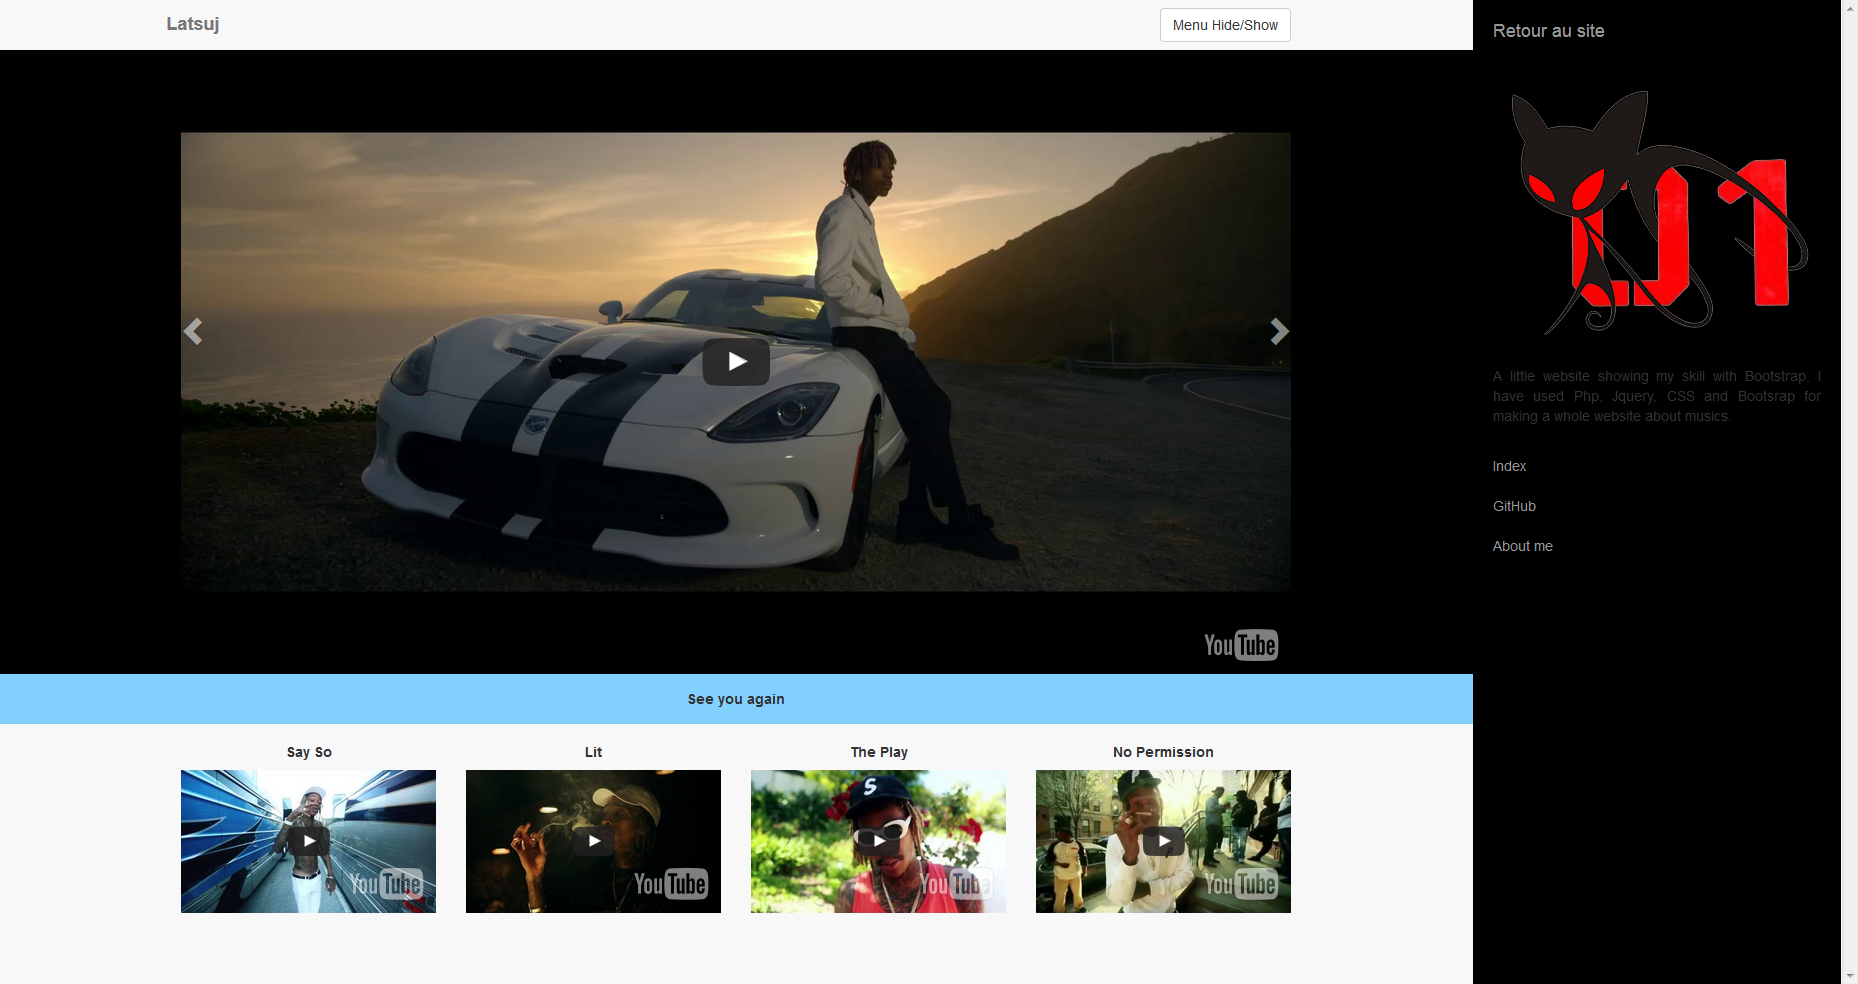
\includegraphics[width=0.48\textwidth]{p2}
  \end{center}
  \vspace{-20pt}
  \caption{Le menu \`a droite sur la version PC}
  \vspace{-10pt}
\end{wrapfigure}
Le menu est la partie \`a droite du site qu'il est possible d'afficher ou non. Par d\'efaut, cette partie est cach\'e pour les m\^eme raison que le bloc d'informations (nombre de points de fixation). Le menu prend aussi une taille diff\'erente en fonction du premier points de rupture que l'on va rencontr\'e lorsque l'on r\'eduit la fen\^etre. Lorsque nous sommes \`a la plus basse r\'esolution le menu prend 100\% de la largeur de la fen\^etre, j'ai trouv\'e que cela \'etait ce qu'il y avait de mieux au niveau utilisation sans ab\^imer la simplicit\'e du site et l'ergonomie.\\
Sur les deux technologies, j'ai utilis\'e la m\^eme technique. L'ensemble du site est englobl\'e dans une balise DIV dont la largeur peux varier via un script JavaScript. De l'autre, le menu est aussi compris dans une balise DIV qui l\`a aussi \`a sa largeur qui pourra varier entre 0 et un nombre d\'ependant de la largeur pris par le contenu du site. \\
\vspace{0.5cm}\\
\fbox{\parbox{0.5\textwidth}{
...\\
<body>\\
\hspace*{0.6cm}<div id="content" style="width:100\%; height:auto; float: left;">\\
\hspace*{1.2cm}...(contenue du site)\\
\hspace*{0.6cm}</div>\\
\hspace*{0.6cm}<div id="menu" style="width:0\%; background:\#000000; float: right;">\\
\hspace*{1.2cm}...(menu)
\hspace*{0.6cm}</div>\\
</body>\\
...
}}
\fbox{\parbox{0.5\textwidth}{
...\\
<body>\\
\hspace*{0.6cm}<my-content>\\
\hspace*{1.2cm}...(contenue du site)\\
\hspace*{0.6cm}</my-content>\\
\hspace*{0.6cm}<my-menu>\\
\hspace*{1.2cm}...(menu)
\hspace*{0.6cm}</my-menu>\\
</body>\\
...
}}
\vspace{0.5cm}\\
Ce code ci-dessus montre la mani\`ere dont j'ai positionn\'e les balises pour r\'ealiser ce menu. Sous Bootstrap, il n'y avait rien pour r\'ealiser cela de mani\`ere "Bootstrapsienne". J'aurai pu mettre le code dans un document style mais j'ai pr\'ef\'er\'e \'eviter cela pour bien montrer que Bootstrap ne permet pas d'effectuer cela de mani\`ere simple. Notons par ailleurs qu'ici, j'ai d\'ecouvert aussi un probl\`eme ennuyant. Il n'est pas possible d'utiliser le syst\`eme de grille de Bootstrap lorsque l'on d\'efinit un \'el\'ement comme \og fixed \fg{}. Ce que je voulais faire au d\'epart, j'ai donc d\^u me raviser.
\vspace{0.5cm}\\
Si vous avez suivi l'int\'egralit\'e des explications ci-dessus, vous \^etes maintenant apte \`a cr\'eer l'application de vos r\^eves en utilisant Bootstrap ou Polymer. Cependant pour d\'ecider quelles applications est la plus adapt\'e \`a vos besoins, il faudra r\'efl\'echir en fonction des utilisateurs que vous viser. Les deux technologies n'\'etant pas support\'e de la m\^eme mani\`ere.
 
\newpage
\section{Outils de d\'eveloppement et test}

\subsection{Outils de d\'eveloppement}

Pour r\'ealiser mon site adaptatif, j'ai eu besoin de plusieurs outils. Chacun ayant une part plus ou moins importante, je vais partir du plus utile dans mon exemple au moins utile mais qui a tout de m\^eme eu un role \`a jouer un moment ou \`a un autre.\\
\begin{wrapfigure}{r}{0.5\textwidth}
  \vspace{-20pt}
  \begin{center}
    
\includegraphics[width=0.48\textwidth]{p22}
  \end{center}
  \vspace{-20pt}
  \caption{Le logo d'\'eclipse}
  \vspace{-10pt}
\end{wrapfigure}

L'outils que j'ai le plus utilis\'e, Eclipse, mon environnement de d\'eveloppement int\'egr\'e pr\'ef\'er\'e. Un IDE (Integrated Development Environment) est un outil qui permet d'augmenter la productivit\'e d'un d\'eveloppeur. Tous les boutons, toutes les fonctions qui se trouvent \`a l'int\'erieur de ce logiciel ont \'et\'e pens\'e pour le d\'eveloppeur. Ayant travaill\'e de nombreuses fois et pour diff\'erents projets avec ce logiciel, j'ai mes propres rep\`eres et cela me permet d'\^etre tr\`es rapide lors de la phase d'impl\'ementation.\\
\begin{wrapfigure}{l}{0.5\textwidth}
  \vspace{-20pt}
  \begin{center}
    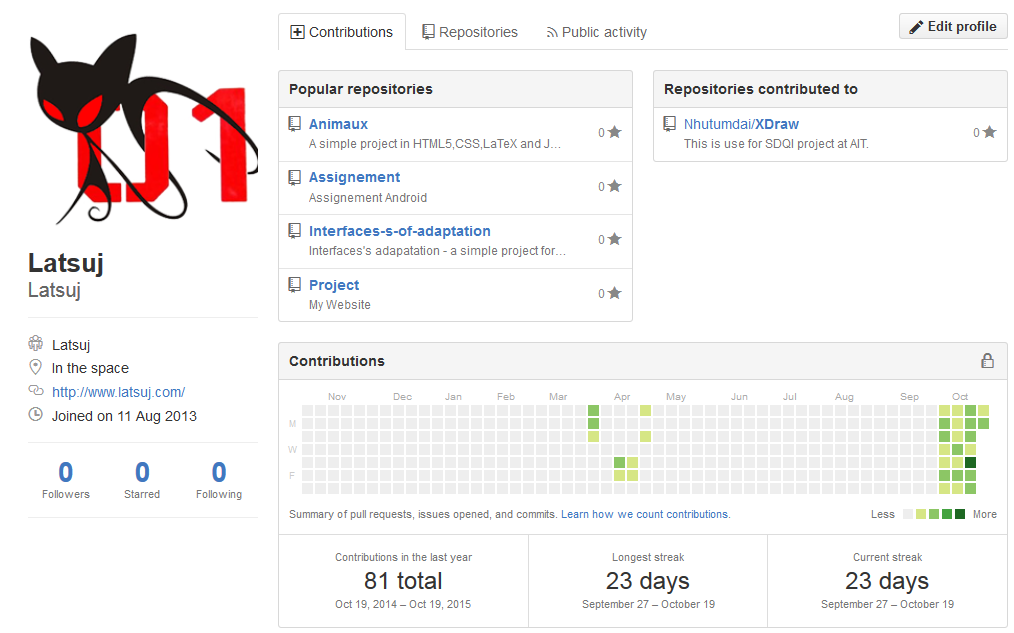
\includegraphics[width=0.48\textwidth]{p23}
  \end{center}
  \vspace{-20pt}
  \caption{Le logo d'\'eclipse}
  \vspace{-10pt}
\end{wrapfigure}

Depuis ce qui s'est pass\'e lors de mon rattrapage en SI3, je ne me s\'epare plus de github lorsque je travaille sur un projet. Si jamais mon PC tombe en panne un jour avant la date limite de rendue (ce qui m'est arriv\'e), j'aurais toujours quelques choses \`a montrer. Cela me permet aussi de voir mes progr\`es sur mon projet. De revenir \`a une version ant\'erieur si jamais une erreur inconnue s'est gliss\'e dans le code... Ce petit logiciel anodin insoup\c{c}onn\'e peut devenir un vrai sauveur de temps si un probl\`eme survient. Je regrette une seule chose : ne pas l'avoir utilis\'e plus t\^ot !
\vspace{0.5cm}\\
\begin{wrapfigure}{r}{0.5\textwidth}
  \vspace{-50pt}
  \begin{center}
    
\includegraphics[width=0.48\textwidth]{p24}
  \end{center}
  \vspace{-20pt}
  \caption{Les APIs}
  \vspace{-10pt}
\end{wrapfigure}

Les API (Application Programming Interface) de Bootstrap ainsi que Polymer ont \'et\'e d'une aide pr\'ecieuse. Une API est un service web qui donne une description plus ou moins pouss\'e sur un programme ou langage. Elles sont souvent accompagn\'es de tutoriels et exemples qui permettent de comprendre rapidement comment fonctionne la technologie. Gr\^ace \`a ces API, j'ai pu d\'evelopper sans trop de difficult\'e mes deux exemples.
\vspace{0.5cm}\\
Enfin, j'ai utilis\'e \`a moindre \'echelle d'autre outils pour finaliser certains d\'etails. J'ai donc utilis\'e \textbf{JQuery} pour effectuer mon carousel sous Polymer. Bootstrap utilise aussi cette biblioth\`eque pour effectuer leur propre carousel. J'ai aussi utilis\'e \textbf{PhpMyAdmin et Wamp}. Comme certaines pages \'etaient identiques en tout points et seul le contenu diff\'erait, j'ai jug\'e bon d'automatiser certaines taches en utilisant un peu de PHP.
\newpage
\subsection{Outils de test}

\hspace*{0.6cm}Pour tester l'affichage et l'adaptation de nos \'el\'ements \`a la fen\^etre, il existe plusieurs voies envisageables. J'ai utilis\'e plusieurs d'entre elles pour effectuer mes tests. La premi\`ere m\'ethode a \'et\'e de modifier la taille de la fen\^etre sous windows.\\

\begin{wrapfigure}{l}{0.5\textwidth}
  \vspace{-25pt}
  \begin{center}
    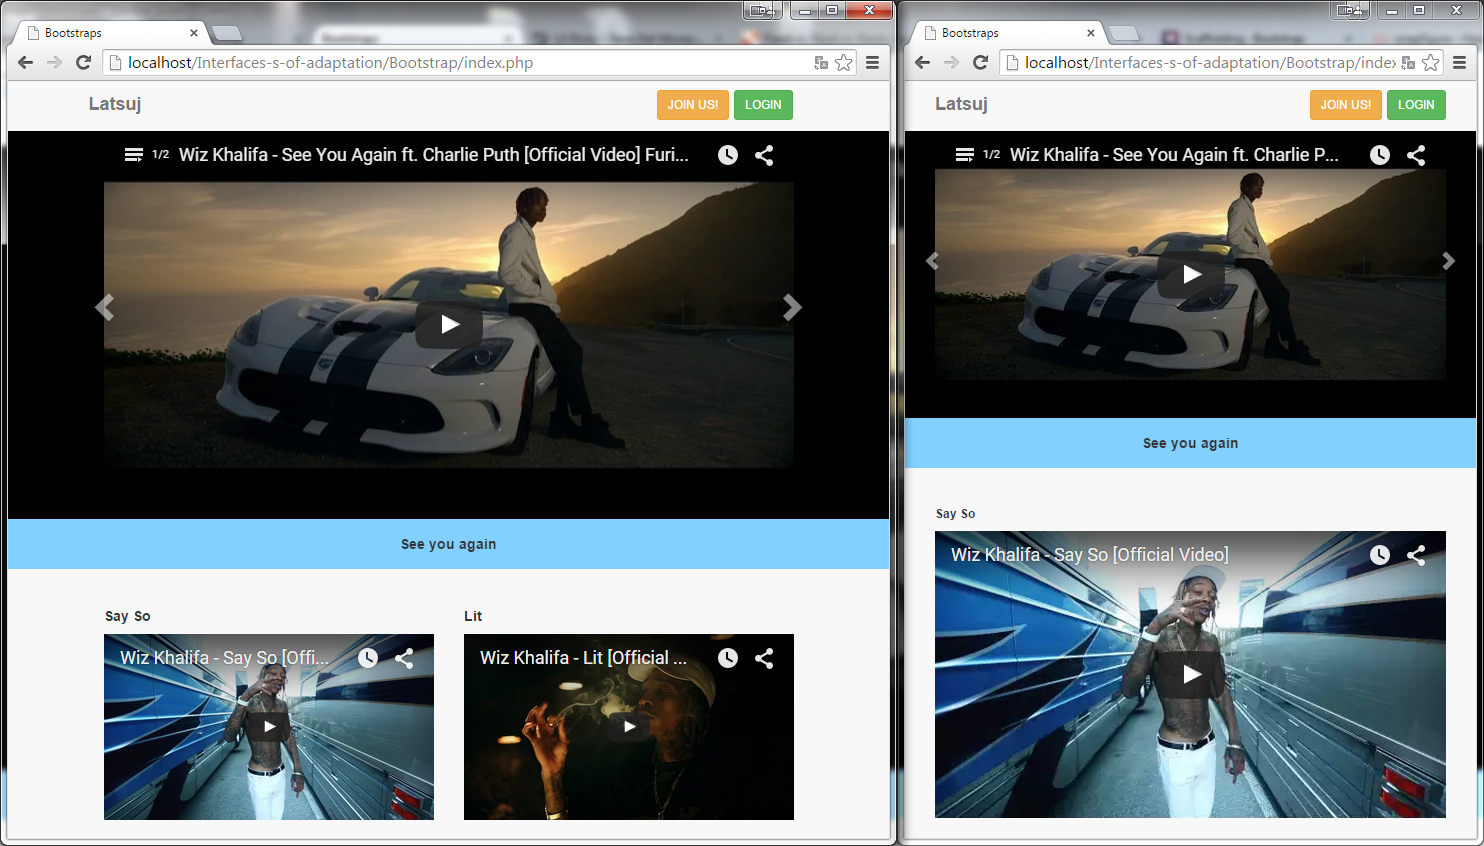
\includegraphics[width=0.48\textwidth]{double}
  \end{center}
  \vspace{-20pt}
  \caption{Redimensionnement de la fen\^etre sous windows}
  \vspace{-10pt}
\end{wrapfigure}

L'exemple de la figure 14 montre le site \`a deux dimensions diff\'erentes. Comme on peux le voir, le site s'adapte bien \`a la largeur de la fen\^etre. Sur la gauche, le site est plus grand. La taille plus grande permet de mettre deux clips vid\'eos l'un \`a cot\'e de l'autre. Sur la droite, le site est plus petit et ne permet de n'afficher qu'un clip vid\'eo par ligne. Les autres \'el\'ements quant \`a eux se redimensionne pour s'adapter \`a la page. J'ai r\'ealis\'e cette op\'eration avec chacun des navigateurs avec Bootstrap. Le r\'esultat obtenue est le m\^eme sur chacun des navigateurs. Avec Polymer, on ne peux test\'e qu'avec quelques navigateurs d\`u au probl\`eme de compatibilit\'e que j'ai \'evoqu\'e pr\'ec\'edemment.\\

\begin{wrapfigure}{r}{0.5\textwidth}
  \vspace{-25pt}
  \begin{center}
    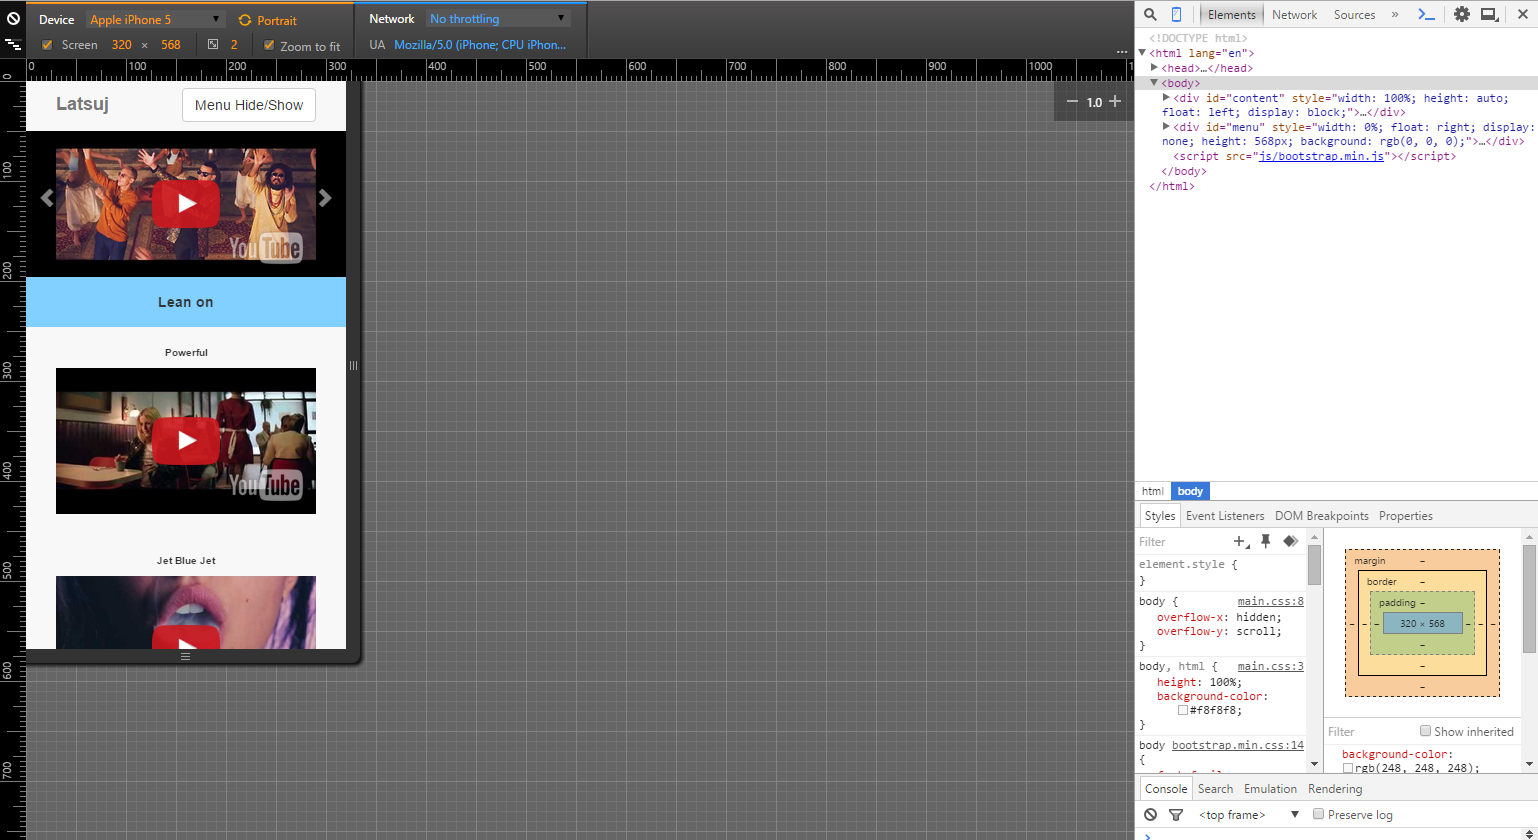
\includegraphics[width=0.48\textwidth]{p16}
  \end{center}
  \vspace{-20pt}
  \caption{Test au format iphone 5}
  \vspace{-10pt}
\end{wrapfigure}

Pour test\'e l'adaptation sur des appareils en particuliers, Google Chrome dispose d'un outil redimensionnant la fen\^etre \`a la dimension exacte d'un appareil en particulier. J'ai utilis\'e cet outil pour voir le r\'esultat sous diff\'erentes tablettes et t\'el\'ephones actuellement sur le march\'e. Pour activer cet option sous le navigateur, il suffit d'appuyer sur F12 puis le bouton repr\'esentant un t\'el\'ephone nomm\'e \og toggle device mode \fg{}.
\vspace{0.5cm}\\
\begin{wrapfigure}{l}{0.5\textwidth}
  \vspace{-25pt}
  \begin{center}
    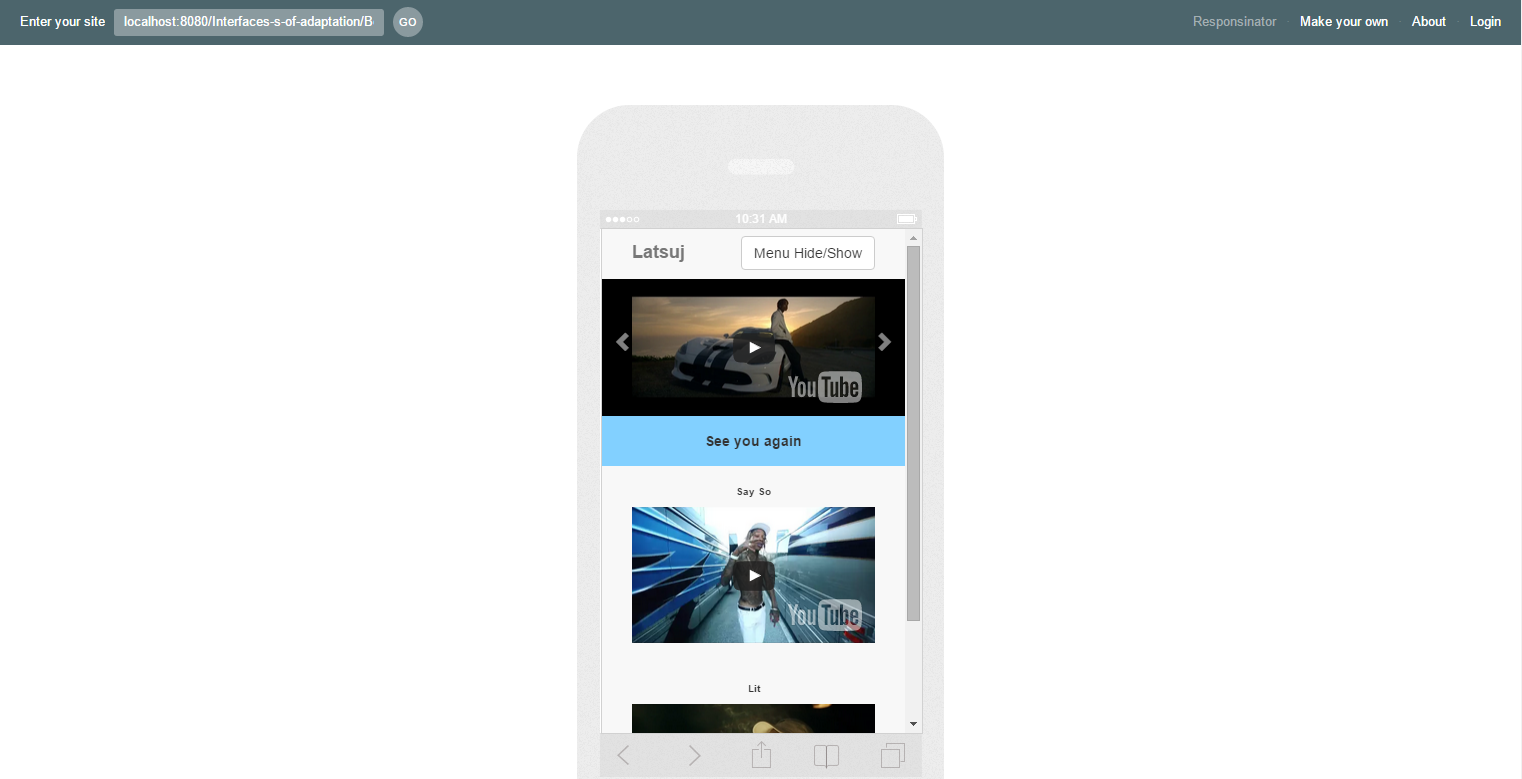
\includegraphics[width=0.48\textwidth]{p17}
  \end{center}
  \vspace{-20pt}
  \caption{Responsinator.com}
  \vspace{-10pt}
\end{wrapfigure} 

Il est aussi possible de passer par des sites qui permettent de tester l'adaptation de nos sites comme responsinator.com. J'ai aussi test\'e mon site sur ce site. On voit sur ce site un grand ensemble d'appareil avec notre site \`a l'int\'erieur. Le seul probl\`eme de cette m\'ethode est qu'il faut charger X fois le m\^eme site, ce qui peut s'av\'erer plut\^ot long si le site en question est relativement lourd.\\

\newpage
\section{Documentations, Outils, liens utiles} 
\textbf{Wikip\'edia}\\
Le site d'o\'u j'ai d\'emarr\'e mes recherches, il contient une bonne d\'efinition des sites RWD.\\
\textit{https://fr.wikipedia.org/wiki/Site\_web\_adaptatif}
\vspace{0.5cm}\\
\textbf{What is a responsible web design ?}\\
Les liens suivant sont les articles ou vid\'eos que j'ai analys\'e pour \'ecrire ce rapport.\\
\textit{https://www.youtube.com/watch?t=133\&v=iSY38POjLYc}
\vspace{0.5cm}\\
\textbf{Ethan Marcotte}\\
Le site du createur du RWD qui montre la diff\'erence entre un site adaptable et un vrai site responsive.\\
\textit{http://alistapart.com/d/responsive-web-design/ex/ex-site-flexible.html}\\
\textit{http://alistapart.com/d/responsive-web-design/ex/ex-site-linearize.html}
\vspace{0.5cm}\\
\textbf{Responsible typesetting}\\
Un article qui traite du responsible typesetting.\\
\textit{http://blog.line0.eu/responsible-typesetting/}
\vspace{0.5cm}\\
\textbf{Fitt's law}\\
La description de la loi de Fitt\\
\textit{https://en.wikipedia.org/wiki/Fitts's\_law}\\
\textit{http://webdesign.tutsplus.com/articles/applying-fitts-law-to-mobile-interface-design--webdesign-6919}
\vspace{0.5cm}\\
\textbf{Media queries}\\
Les medias queries sont int\'erressants mais limit\'es. Le futur serait plutot du cot\'e des \'el\'ements queries (media queries sur \'el\'ements et non par rapport au viewport).\\
\textit{http://ianstormtaylor.com/media-queries-are-a-hack/}\\
\textit{http://www.smashingmagazine.com/2013/06/media-queries-are-not-the-answer-element-query-polyfill/}
\vspace{0.5cm}\\
\textbf{Le champs visuels}\\
Le champs visuels est une aide pr\'ecieuse pour designer une interface.\\
\textit{http://sophie.raufaste.free.fr/Saccades\%20fixations\%20et\%20champs\%20visuel.htm}\\

\end{document}
